%                                     MMMMMMMMM        
%                                                                             
%  MMO    MM   MMMMMM  MMMMMMM   MM    MMMMMMMM   MMD   MM  MMMMMMM MMMMMMM   
%  MMM   MMM   MM        MM     ?MMM              MMM$  MM  MM         MM     
%  MMMM 7MMM   MM        MM     MM8M    MMMMMMM   MMMMD MM  MM         MM     
%  MM MMMMMM   MMMMMM    MM    MM  MM             MM MMDMM  MMMMMM     MM     
%  MM  MM MM   MM        MM    MMMMMM             MM  MMMM  MM         MM     
%  MM     MM   MMMMMM    MM   MM    MM            MM   MMM  MMMMMMM    MM
%
%
%            - META-NET Language Whitepaper | Portuguese content -
% 
% ----------------------------------------------------------------------------

\begin{document}

\maketitle

\null
\pagestyle{empty} 

\makefundingnotice

\pagenumbering{Roman} 
\setcounter{page}{5}
\pagestyle{scrheadings}

\cleardoublepage

% --------------------------------------------------------------------------
\bsection*{Prefácio --- Preface}

\begin{Parallel}[c]{78mm}{78mm}
\ParallelLText{\selectlanguage{portuguese}
Este livro branco faz parte de uma série que promove o conhecimento sobre as Tecnologias da Linguagem e o seu potencial. É particularmente dirigido a educadores, jornalistas, políticos e comunidades linguísticas, entre outros.

A disponibilidade e a utilização das Tecnologias da Linguagem na Europa variam consoante as línguas. Por conseguinte, as ações que são necessárias para apoiar a investigação e o desenvolvimento destas tecnologias também são diferentes para cada língua. Estas ações dependem de vários fatores, tais como a complexidade de uma determinada língua e a dimensão da sua comunidade. 

META-NET, um projeto da Rede de Excelência da Comissão Europeia, levou a cabo, nesta série de Livros Brancos, uma análise dos atuais recursos linguísticos e tecnologias disponíveis (p.~\pageref{whitepaperseries}). A análise focou as 23 línguas oficiais europeias, bem como outras línguas importantes na Europa, a nível nacional e regional. Os resultados apontam a existência de significativas lacunas em determinadas áreas de investigação para cada língua. Análises e avaliações mais detalhadas da situação atual poderão ajudar a maximizar o impacto de uma investigação adicional e a minimizar quaisquer riscos.

O projeto META-NET abrange, em Novembro de 2011, 54 centros de investigação de 33 países (p.~\pageref{metanetmembers}), que estão a trabalhar com as partes interessadas de empresas comerciais, agências governamentais, indústria, instituições de investigação, empresas de \textit{software}, fornecedores de tecnologia e universidades europeias. Em conjunto, pretendem criar uma visão tecnológica comum, desenvolvendo, ao mesmo tempo, um plano estratégico de investigação que mostrará de que modo as aplicações na área das Tecnologias da Linguagem poderão vir a suprir algumas lacunas na investigação, até 2020.}

\ParallelRText{\selectlanguage{english}
This white paper is part of a series that promotes knowledge about language technology and its potential. It addresses journalists, politicians, language communities, educators and others. 

The availability and use of language technology in Europe varies between languages. Consequently, the actions that are required to further support research and development of language technologies also differs. The required actions depend on many factors, such as the complexity of a given language and the size of its community.

META-NET, a Network of Excellence funded by the European Commission, has conducted an  analysis of current language resources and technologies in this white paper series (p.~\pageref{whitepaperseries}). The analysis focused on the 23 official European languages as well as other important national and regional languages in Europe. The results of this analysis suggest that there are tremendous deficits in technology support and significant research gaps for each language. The given detailed expert analysis and assessment of the current situation will help maximise the impact of additional research.

As of November 2011, META-NET consists of 54 research centres from 33 European countries (p.~\pageref{metanetmembers}). META-NET is working with stakeholders from economy (Software companies, technology providers, users), government agencies, research organisations, non-governmental organisations, language communities and European universities. Together with these communities, META-NET is creating a common technology vision and strategic research agenda for multilingual Europe 2020.} 
\ParallelPar
\end{Parallel}

% --------------------------------------------------------------------------

\cleardoublepage

\bsection*{Índice --- Table of Contents}

\tableofcontents

\addtocontents{toc}{\protect\thispagestyle{empty}\protect}
\addtocontents{toc}{{\Large\textsf{\centerline{A LÍNGUA PORTUGUESA NA ERA DIGITAL}}\par}}

% --------------------------------------------------------------------------

\cleardoublepage

\setcounter{page}{1}
\pagenumbering{arabic} 
\pagestyle{scrheadings}

\ssection[Sumário]{Sumário}

\selectlanguage{portuguese}

\begin{multicols}{2}
Durante os últimos 60 anos, a Europa transformou-se numa importante estrutura política e económica, apesar da sua diversidade cultural e linguística. Isto significa que, do português ao polaco e do italiano ao islandês, os cidadãos europeus são inevitavelmente confrontados com barreiras linguísticas ao comunicarem entre si, tanto no dia-a-dia como nas esferas dos negócios e da política. As instituições da União Europeia gastam cerca de mil milhões de euros anuais na manutenção da sua política de multilinguismo, ou seja, na tradução de textos e na interpretação de comunicação oral. Terá isto, porém, de ser um fardo? As modernas Tecnologias da Linguagem (TL) e a investigação em linguística podem dar uma importante contribuição para ultrapassar as barreiras linguísticas. No futuro, quando combinadas com dispositivos e aplicações inteligentes, as TL terão a capacidade de ajudar os europeus a falar mais facilmente uns com os outros e a fazer negócios, mesmo que não tenham uma língua em comum.

\boxtext{As Tecnologias da Linguagem constroem pontes para o futuro da Europa.}

As barreiras linguísticas podem provocar impasses nos negócios e trazer dificuldades, tanto à economia portuguesa como a outras economias europeias. Isto pode ser especialmente prejudicial no caso das PME, que não têm os meios financeiros para inverter esta situação. A única alternativa a esta Europa multilingue (embora tal seja impensável) seria permitir que um único idioma assumisse uma posição dominante, substituindo todos os outros.

Uma forma clássica de ultrapassar a barreira da língua consiste na aprendizagem de línguas estrangeiras. Todavia, sem um apoio tecnológico, dominar as 23 línguas oficiais, bem como as restantes 60 línguas faladas na Europa, é um obs\-tá\-cu\-lo intransponível para os cidadãos, a economia, o debate político e o progresso científico europeus.

A solução passa, então, por desenvolver tecnologias-chave. Estas oferecerão aos atores europeus enormes vantagens, não apenas dentro do Mercado Comum Europeu, mas também nas relações comerciais com outros países, especialmente com as economias emergentes. Para atingir este objetivo e preservar a diversidade cultural e linguística da Europa, é necessário, em primeiro lugar, fazer uma análise sistemática das particularidades linguísticas de todas as línguas europeias e do estado atual das tecnologias de suporte criadas para estas. As soluções possibilitadas pelas TL acabarão por servir como uma ponte única entre as diferentes línguas europeias.

\boxtext{As Tecnologias da Linguagem como uma chave para o futuro.}

 A tradução automática e as ferramentas de processamento da fala atualmente existentes no mercado estão ainda muito distantes do ambicioso objetivo acima descrito. Nesta área, os atores dominantes são sobretudo empresas privadas, com fins lucrativos, sediadas na América do Norte. Já no final dos anos 70, a União Europeia percebeu a extrema importância das TL como forma de contribuir para a unidade europeia e começou a financiar os primeiros projetos de investigação, como foi o caso do EUROTRA. Simultaneamente, foram criados projetos a nível nacional que produziram bons resultados, mas que nunca conduziram a uma ação europeia concertada. Em contraste com este esforço de financiamento altamente seletivo, outras sociedades multilingues, como a Índia (22 línguas oficiais) e a África do Sul (11 línguas oficiais), criaram, recentemente, programas nacionais a longo prazo para a investigação da linguagem e desenvolvimento tecnológico.

Atualmente, o trabalho das figuras de proa na área das TL depende de abordagens estatísticas imprecisas que não utilizam métodos e conhecimentos linguísticos mais profundos. Por exemplo, as frases são automaticamente traduzidas através da comparação de uma nova frase com milhares de frases anteriormente traduzidas de forma manual. Assim, a qualidade do \textit{output} depende, em grande medida, da quantidade e da qualidade do \textit{corpus} que serve de amostra. Embora a tradução automática de frases simples em línguas com uma quantidade suficiente de textos disponíveis possa alcançar resultados úteis, estes métodos estatísticos superficiais estão condenados ao fracasso no caso das línguas com um conjunto de material de amostra muito menor ou no caso de frases com estruturas complexas. 

Neste contexto, a União Europeia decidiu financiar projetos como o EuroMatrix e o EuroMatrixPlus (desde 2006) e o iTranslate4 (desde 2010) que levam a cabo pesquisas básicas e aplicadas e geram recursos com o objetivo de criar soluções de TL de alta qualidade para todas as línguas europeias. A\-na\-li\-sar as propriedades estruturais mais profundas das línguas é a única forma de assegurar o desenvolvimento de aplicações que tenham um bom desempenho para o conjunto das línguas europeias.

A investigação europeia nesta área já alcançou uma série de sucessos. Por exemplo, os serviços de tradução da União Europeia utilizam agora o MOSES, um \textit{software} de tradução automática, disponível em código aberto, que foi sobretudo desenvolvido através de projetos europeus de investigação. Contudo, ao invés de se basear nos resultados dos seus projetos de investigação para progredir, a Europa apresenta ainda uma tendência para desenvolver atividades de pesquisa de forma isolada e, consequentemente, com um impacto menor no mercado. O valor económico até mesmo dos primeiros esforços reflete-se no número de \textit{spin-offs}. Uma empresa como a Trados, fundada em 1984, foi vendida em 2005 a uma empresa sediada no Reino Unido, a SDL.

\boxtext{As Tecnologias da Linguagem ajudam a unificar a Europa.}

Com base nos conhecimentos adquiridos até agora, parece que, no âmbito das TL, o método híbrido que mistura o processamento profundo com métodos estatísticos será capaz de criar pontes entre todas as línguas da Europa e, até, de ir mais além. Como mostra esta série de Livros Brancos, há uma di\-fe\-ren\-ça dramática entre os vários países europeus no que diz respeito às soluções disponíveis e ao estado da investigação na área da linguagem. Apesar de o português ser uma das línguas mais faladas no mundo, necessita de muito mais investigação antes de se obterem soluções de TL verdadeiramente eficazes para o uso quotidiano.

A longo prazo, o objetivo da META-NET é a criação de TL de alta qualidade para todas as línguas, a fim de alcançar a unidade política e económica através da diversidade cultural. A tecnologia ajudará a derrubar as barreiras existentes e a construir pontes entre as línguas europeias. Isto vai exigir de todas as partes interessadas – na política, na investigação, nos negócios e na sociedade – uma união de esforços com vista ao futuro.

Esta série de Livros Brancos complementa outras ações estratégicas levadas a cabo pela META-NET (veja o anexo para uma visão mais geral). Informações atualizadas, como a versão mais recente do documento\cite{Meta1}  ou a Agenda Estratégica de Investigação, podem ser encontradas no site da META-NET: http://www.meta-net.eu
\end{multicols}

\clearpage

% --------------------------------------------------------------------------

\ssection[Um risco para as nossas línguas e um desafio para as Tecnologias da Linguagem]{Um risco para as nossas línguas \newline e um desafio para as Tecnologias da Linguagem}

\begin{multicols}{2}

Somos hoje testemunhas de uma revolução digital que está a ter um impacto radical na comunicação e na sociedade. Os recentes desenvolvimentos nas áreas da informação digital e das tecnologias da comunicação são por vezes comparados com a invenção da imprensa por Gutenberg. O que pode esta analogia dizer-nos sobre o futuro da sociedade de informação europeia e sobre as nossas línguas em particular?

\boxtext{Estamos a testemunhar uma revolução digital comparável à invenção da imprensa por Gutenberg.}

Depois da invenção de Gutenberg, os avanços na comunicação e na partilha de conhecimentos foram realizados mediante alguns esforços, como a tradução da Bíblia do Latim para as línguas vernáculas da Europa, por Lutero. Nos séculos seguintes, foram desenvolvidas novas técnicas para melhor lidar com o processamento da linguagem e a partilha de co\-nhe\-ci\-men\-to:

\medskip
\begin{itemize}
   \item a padronização ortográfica e gramatical das principais línguas permitiu a rápida divulgação de novas perspetivas científicas e intelectuais;
      \item o desenvolvimento das línguas oficiais tornou possível aos cidadãos comunicarem dentro de certas fronteiras (muitas vezes políticas);
      \item o ensino e a tradução de línguas permitiram uma partilha de conhecimento entre línguas;
      \item a criação de diretrizes editoriais e bibliográficas garantiu a qualidade e a disponibilidade do material impresso;
      \item o surgimento de diferentes meios de comunicação, como jornais, rádio, televisão, livros e outros suportes e formatos, veio dar resposta às diferentes necessidades de comunicação. 
\end{itemize}

 Nos últimos vinte anos, as tecnologias da informação ajudaram a automatizar e a facilitar muitos dos processos:

\begin{itemize}
      \item os programas avançados de edição de texto (\textit{desktop publishing software}) substituem a datilografia e a composição tipográfica;
      \item as projeções de transparências dão lugar às apresentações em Powerpoint;
      \item o correio eletrónico permite receber e enviar do\-cu\-men\-tos de forma mais rápida do que o fax;
      \item o Skype permite a realização de chamadas de telefone gratuitas ou a preços reduzidos pela internet, bem como de videoconferências;
      \item os formatos de codificação de áudio e vídeo facilitam a troca de conteúdos multimédia;
      \item os motores de busca sugerem palavras-chave baseadas nos acessos a páginas Web;
      \item os serviços de tradução online, como o serviço gratuito do Google, produzem traduções de uma forma rápida e aproximada ao texto original;
      \item as plataformas de redes sociais como o Facebook, o Twitter e o Google+  facilitam a comunicação, a colaboração e a partilha de informação.
\end{itemize}

 Apesar de estas ferramentas e aplicações serem úteis, ainda não são capazes de suportar uma sociedade europeia multilingue e sustentável para todos, onde informação e bens possam circular livremente.

\subsection{Fronteiras linguísticas travam a sociedade de in\-for\-ma\-ção eu\-ro\-peia}
  
Não podemos saber exatamente como será o futuro da sociedade de informação. Há, porém, uma forte probabilidade de que a revolução nas tecnologias da comunicação venha a aproximar pessoas que falam diferentes línguas em novos meios. Esta situação pressiona os utilizadores a aprenderem novas línguas e pressiona sobretudo os programadores a criarem novas aplicações tecnológicas para permitir a compreensão mútua e o acesso a conhecimento compartilhável. Este espaço económico e de informação global envolve a interação entre línguas, falantes e conteúdos no âmbito de novos meios de comunicação. A recente popularidade das redes sociais (Wikipédia, Facebook, Twitter, YouTube e, mais recentemente, o Google+) é apenas o início. 

\boxtext{A economia global e o espaço de informação colocam-nos \mbox{diante} de mais línguas, falantes e conteúdos.}

Hoje, podemos transmitir gigabytes de texto para todo o mundo em poucos segundos, antes de percebermos que o conteúdo está redigido numa língua que não entendemos. De acordo com um recente relatório da Comissão Europeia, 57\% dos utilizadores da internet compram bens e serviços em línguas que não a sua (o inglês é a língua estrangeira mais usada, seguido pelo francês, alemão e espanhol). 55\% dos utilizadores leem conteúdos numa língua estrangeira, enquanto apenas 35\% utilizam outra língua para escrever mensagens de correio electrónico ou colocar comentários na internet\cite{EC1}. Há alguns anos atrás, o inglês era a língua franca na internet – a maior parte dos conteúdos estavam de facto em inglês – mas agora a si\-tua\-ção mudou radicalmente. A quantidade de conteúdos \textit{online} noutras línguas europeias (assim como em línguas asiáticas e do Médio Oriente) aumentou exponencialmente.

Surpreendentemente, esta divisão digital criada pelas fronteiras linguísticas não recebe muita atenção pública. Ainda assim, levanta-se uma questão premente: “que línguas europeias vão prosperar na informação em rede e na sociedade do co\-nhe\-ci\-men\-to, e quais estão condenadas a desaparecer?”

\subsection{As nossas línguas em risco}

 Embora a imprensa escrita tenha ajudado a intensificar a troca de informação na Europa, também levou à extinção de muitas línguas europeias. Línguas regionais e minoritárias raramente foram impressas, como o \textit{Cornish} e o Dálmata, e foram reduzidas a formas orais de transmissão, o que limitou o seu uso. No futuro, terá a internet o mesmo impacto nas nossas línguas?

As cerca de 80 línguas da Europa são um dos mais ricos e importantes bens culturais e uma parte vital do seu modelo social único\cite{EC2}. Enquanto línguas como o inglês e o espanhol sobreviverão no mercado digital emergente, muitas línguas europeias poderão tornar-se irrelevantes para uma sociedade em rede. Isso enfraqueceria a posição global da Europa e iria contra o objetivo estratégico da participação igualitária de todos os cidadãos europeus, independentemente da sua língua. De acordo com um relatório da UNESCO sobre multilinguismo, as línguas são um meio essencial para o exercício dos direitos fundamentais, como a expressão política, a educação e a participação em sociedade\cite{Unesco1}.

\boxtext{A multiplicidade de línguas é também uma parte vital do êxito social da Europa.}

\subsection{A tecnologia da linguagem é uma tecnologia chave}

 No passado, os esforços de investimento para a preservação das línguas concentraram-se no ensino e na tradução. De acordo com uma estimativa, o Mercado Europeu de tradução, interpretação, localização de \textit{software} e preparação de \textit{websites} para o mercado global (\textit{website globalisation}) foi de 8,4 mil milhões de euros em 2008 e deverá crescer 10\% por ano\cite{EC3}. No entanto, este número abrange apenas uma pequena parte das necessidades atuais e futuras da comunicação entre línguas. A solução mais atraente para garantir uma ampla cobertura das várias línguas na Europa do futuro é a utilização de tecnologia adequada, tal como usamos a tecnologia nas áreas da energia e dos transportes e para apoiar cidadãos com necessidades especiais, entre outros casos.

\boxtext{A Europa precisa de tecnologias da linguagem robustas e acessíveis para todas as línguas europeias.}

As Tecnologias da Linguagem Digital (segmentação de todas as formas de texto escrito e discurso falado) ajudam as pessoas a colaborar, a conduzir negócios, a partilhar conhecimentos e a participar em debates sociais e políticos, independentemente das barreiras linguísticas e das competências informáticas de cada um. As Tecnologias da Linguagem (TL) funcionam muitas vezes de forma invisível dentro de sistemas de \textit{software} complexos, ajudando-nos a:

\begin{itemize}
  \item encontrar informação na internet, através de um motor de busca;
      \item verificar a ortografia e a gramática num processador de texto;
      \item ver as recomendações para um produto numa loja \textit{online};
      \item seguir as indicações verbais de um sistema de navegação automóvel;
      \item traduzir páginas da internet com um serviço \textit{online}.
\end{itemize}

As TL são compostas por um conjunto de aplicações básicas que permitem a sua aplicação num quadro mais vasto. O objetivo dos Livros Brancos da META-NET é o de perceber o nível de desenvolvimento destas aplicações para cada uma das línguas europeias.

\boxtext{A Europa precisa de Tecnologias da Linguagem robustas e acessíveis para todas as línguas europeias.}

Para manter a posição na linha da frente da inovação mundial, a Europa necessitará de TL que estejam adaptadas a todas as línguas europeias e que sejam igualmente robustas, acessíveis e totalmente integradas em plataformas informáticas. Sem as TL não nos será possível, enquanto utilizadores, alcançar uma experiência realmente interativa, multimédia e multilingue num futuro próximo.

\subsection{Oportunidades para as Tecnologias da Linguagem}

O desenvolvimento da imprensa, isto é, a duplicação rápida de uma imagem de texto (uma página), foi um avanço tecnológico fundamental. Antes, era necessário fazer o trabalho árduo de pesquisar, ler, traduzir e resumir o conhecimento. Foi preciso esperar até Edison para gravar a língua falada - e esta tecnologia permitia apenas fazer cópias analógicas.

As Tecnologias da Linguagem Digital podem agora automatizar muitos dos processos de tradução, produção de conteúdos e gestão de conhecimentos para todas as línguas europeias. Permitem igualmente desenvolver interfaces baseadas na língua/fala para eletrodomésticos, máquinas, veículos, computadores e robôs. As aplicações industriais e comerciais ainda estão num estádio inicial de desenvolvimento, mas os resultados em Investigação e Desenvolvimento (I\&D) estão a criar verdadeiras janelas de oportunidades. Por exemplo, a Tradução Automática já é razoavelmente precisa em certos domínios específicos e algumas aplicações experimentais já fornecem informação multilingue e gestão do conhecimento, bem como a possibilidade de produzir conteúdos em várias línguas europeias.

Como a maioria das tecnologias, as primeiras aplicações para as línguas, como as interfaces de voz baseadas no utilizador e os sistemas de diálogo, foram desenvolvidas para domínios altamente especializados e apresentavam limitações de desempenho. Contudo, existem grandes oportunidades de mercado nas indústrias da educação e do entretenimento para a integração das TL em jogos, em \textit{sites} do património cultural, pacotes de jogos e\-du\-ca\-ti\-vos, bibliotecas, simuladores e programas de treino. Os serviços de informação móvel, os programas de aprendizagem de uma língua assistida por computador, os ambientes de \textit{e-learning}, as ferramentas de autoavaliação e os programas de deteção de plágios são apenas alguns dos exemplos onde estas tecnologias podem desempenhar um papel importante. A popularidade das redes sociais, como o Twitter e o Facebook, sugerem uma maior necessidade de sofisticação das TL para permitir uma monitorização de mensagens, resumir discussões, sugerir tendências de opinião, detetar respostas emocionais, identificar infrações aos direitos de autor ou seguir pistas de uso indevido.

\boxtext{As Tecnologias da Linguagem ajudam a superar os obstáculos colocados pela diversidade linguística.} 

As TL representam uma enorme oportunidade para a União Europeia. Podem ajudar a resolver a complexa questão do multilinguismo na Europa, nomeadamente o facto de diferentes línguas coexistirem naturalmente nos negócios, nas organizações e nas escolas. Todavia, os cidadãos têm a necessidade de comunicar para além destas fronteiras linguísticas que atravessam o Mercado Comum Europeu e as TL podem ajudar a superar os obstáculos que ainda existem, permitindo o uso livre e ilimitado das diversas línguas. Pensando a longo prazo, as inovadoras TL multilingues europeias serão uma referência para os nossos parceiros globais e as suas comunidades multilingues. As TL podem ser vistas como uma forma de “tecnologia de apoio” que ajuda a ultrapassar os obstáculos da diversidade linguística e tornar as comunidades linguísticas mais acessíveis umas para as outras.

Finalmente, um campo ativo de investigação é o uso das TL em operações de resgate em locais de acidente, onde um bom desempenho pode ser uma questão de vida ou de morte. Perante tal cenário, robôs inteligentes com capacidades multilingues poderão, no futuro, salvar vidas.

\subsection{Desafios para as Tecnologias da Linguagem}

 Embora tenha havido um progresso considerável na área das TL nos últimos anos, o atual ritmo de progresso tecnológico e de inovação de produtos é muito lento. As tecnologias com maior utilização, como os corretores de gramática e ortografia em processadores de texto, são normalmente monolingues e estão apenas disponíveis para um pequeno conjunto de idiomas. Os serviços de tradução automática \textit{online}, apesar de serem úteis em gerar rapidamente aproximações ao conteúdo de documentos, apresentam dificuldades quando são exigidas traduções mais precisas e complexas. 

\boxtext{O ritmo \mbox{actual} do progresso tecno\-ló\-gi\-co é muito lento.}

Devido à complexidade da linguagem humana, modelar os nossos idiomas em \textit{software} e testá-los no mundo real é um longo e oneroso negócio, que exige compromissos de financiamento sustentado. A Europa deve, portanto, manter o seu papel pioneiro perante os desafios da tecnologia numa comunidade multilingue, criando novos métodos para acelerar o desenvolvimento de forma global. Este objectivo pode ser conseguido através de desenvolvimentos computacionais, bem como de técnicas como o \textit{crowdsourcing}.

\subsection{Aquisição da linguagem por seres humanos e por máquinas}

 Para ilustrar como os computadores lidam com a linguagem e as razões pelas quais é difícil pro\-gra\-má-los para esse efeito, vamo-nos centrar, ainda que brevemente, na forma como os seres humanos adquirem as suas primeira e segunda línguas, e depois ver como funcionam os sistemas de TL.

Os seres humanos adquirem competências linguísticas de dois modos diferentes. Os bebés aprendem uma língua ouvindo as interações entre os pais, irmãos e outros membros da família. A partir dos dois anos (sensivelmente), as crianças produzem as suas primeiras palavras e frases curtas. Isto só é possível porque os humanos têm a predisposição genética para imitar e racionalizar o que ouvem.

\boxtext{Os seres humanos adquirem competências linguísticas de dois modos diferentes: através de exemplos e através de regras linguísticas.}

Aprender uma segunda língua numa idade mais avançada exige um esforço maior, sobretudo quando quem aprende não está inserido numa comunidade de falantes dessa língua. Na escola, as línguas estrangeiras são normalmente adquiridas através do ensino da estrutura gramatical, vocabulário e ortografia, utilizando exercícios que descrevem conhecimentos linguísticos em termos de regras abstratas, tabelas e exemplos. Com a idade, vai-se tornando cada vez mais difícil aprender uma língua estrangeira.

Os dois principais sistemas de TL  “adquirem” capacidades linguísticas de forma similar. As abordagens estatísticas (ou \textit{data-driven}) permitem obter conhecimentos linguísticos a partir de vastas coleções de exemplos concretos de textos. Embora seja suficiente usar textos numa única língua para, por exemplo, treinar um corretor ortográfico, têm, contudo, de estar disponíveis textos paralelos em duas (ou mais) línguas para o treino de um sistema de tradução automática. Em seguida, o algoritmo de aprendizagem automática “aprende” os padrões de como as palavras, expressões e frases completas são traduzidas.

Esta abordagem estatística pode exigir milhões de frases e a qualidade do seu desempenho aumenta com a quantidade de textos analisados. Esta é uma das razões pelas quais os fornecedores de motores de busca pretendem recolher o máximo de material escrito possível. A correção ortográfica em processadores de texto e serviços como o Google Search e o Google Translate dependem das abordagens estatísticas. A grande vantagem da estatística é que a máquina tem uma rápida aprendizagem em séries contínuas de ciclos de treino, mesmo que a qualidade possa variar de forma arbitrária.

A segunda abordagem às TL, e à Tradução Automática em particular, é a construção de sistemas baseados em regras. Especialistas nas áreas da Linguística, Linguística Computacional e Ciências Computacionais têm de, primeiro, codificar a análise gramatical (regras de tradução) e compilar listas de vocabulário (léxicos). Isto requer muito tempo e trabalho. Alguns dos principais sistemas baseados em regras de tradução automática estão em constante desenvolvimento há mais de 20 anos. A grande vantagem de sistemas baseados em regras é que os peritos têm um controlo mais detalhado sobre o processamento da linguagem. Isto torna possível corrigir de forma sistemática os erros no programa e dar uma resposta detalhada ao utilizador, especialmente quando sistemas baseados em regras são usados para a aprendizagem de línguas. Contudo, devido ao alto custo deste trabalho, as TL baseadas em regras só foram desenvolvidas para certos idiomas.

Como os pontos fortes e fracos de dados estatísticos e sistemas baseados em regras tendem a ser complementares, a investigação atual concentra-se em abordagens híbridas que combinam as duas metodologias. No entanto, estas abordagens têm tido até agora menos sucesso nas aplicações industriais do que nos centros de investigação.

Como vimos neste capítulo, muitas aplicações amplamente utilizadas na atual sociedade de informação dependem fortemente das TL. Devido à sua comunidade multilingue, isto é particularmente verdadeiro no espaço económico e de informação da Europa. Embora as TL tenham feito progressos consideráveis nos últimos anos, há ainda um enorme potencial para melhorar os resultados obtidos. Na secção seguinte, vamos descrever o papel do português na sociedade europeia de informação e avaliar o estado atual das TL para a língua portuguesa.

\end{multicols}

\clearpage

% --------------------------------------------------------------------------

\ssection[O português na sociedade de \mbox{informação} \mbox{europeia}]{O português na sociedade de informação \newline europeia}

\begin{multicols}{2}

\subsection{Factos gerais}

O português é, em número de falantes, a terceira língua europeia no mundo, com cerca de 200 milhões de falantes nativos, e um total de 220 milhões de falantes (como língua materna e língua segunda) em 4 continentes: Europa, América, África e Ásia\cite{observatorio} \cite{ethnologue}.

\boxtext{O português é a terceira língua europeia mais falada no mundo, com cerca de 220 milhões de falantes.}

É a língua oficial de Portugal, Brasil, Angola, Cabo Verde, Guiné-Bissau, Moçambique, São Tomé e Príncipe, Timor Leste, Macau, e, desde 2010, da Guiné Equatorial. 

Devido ao fluxo de emigração \cite{stat1}\cite{obsemig}, o português é também falado por comunidades portuguesas presentes em muitos países, ocupando em alguns deles uma importante posição entre o ranking da população estrangeira. É o caso, na Europa, do Luxemburgo (cerca de 25\% da população), Andorra (à volta de 11\%), França, Alemanha, Reino Unido, Suíça, Espanha e Bélgica\cite{linha}. 

O português é uma das línguas oficiais da União Europeia, do Mercosul (união económica que inclui o Brasil e outros países sul-americanos) e da União Africana. Com o desenvolvimento da alfabetização nas ex-colónias em África e Timor Leste, assim como em Macau, o português tem um grande potencial de crescimento como língua segunda. 

As expedições e o comércio costeiro que Portugal manteve durante vários séculos tiveram contrapartidas linguísticas: o português incorporou palavras de origem africana, ameríndia e asiática, mas também deu a sua contribuição lexical para muitas línguas no mundo, incluindo a língua franca do Mar Mediterrâneo, e vários pidgins e crioulos do Oceano Atlântico, Oceano Pacífico e Oceano Índico\cite{andrade} \cite{camoes}. 

Em Portugal, a divisão geográfica dos dialetos\cite{cintra} distingue os dialetos do Centro-Sul dos dialetos do Norte. As diferenças são facilmente identificáveis ao nível da fonética e fonologia e ao nível lexical, embora todos os dialetos sejam mutuamente compreensíveis (possivelmente com a exceção de alguns dialetos das ilhas dos Açores). Os dialetos do Norte podem ser distinguidos pela ausência da distinção fonológica entre /b/ e /v/, com prevalência do /b/; pela preservação de antigos ditongos; e pela existência de fricativas ápicoalveolares. 

Quanto ao Brasil, dada a dimensão geográfica deste país, não é viável apresentar aqui as suas variedades linguísticas. Por razões geográficas, políticas e sociais, também não é possível falar de uma variedade padrão do português do Brasil. Em vez disso, os especialistas tendem a falar em “normas urbanas cultas”, que apresentam diferenças significativas relativamente à norma do português europeu. 

As variedades africanas do português também são diferentes da europeia, mas as diferenças não são tão acentuadas como as que se observam no português do Brasil, e partilham até algumas características com esta variedade. A situação das variedades africanas diverge muito entre si: enquanto em Angola e Moçambique o número de falantes de português tem vindo a aumentar desde a independência em relação a Portugal, noutros casos, como São Tomé e Princípe e Cabo Verde, utiliza-se amplamente o crioulo, e o português é adquirido como língua segunda.


\subsection{Particularidades da língua portuguesa}

O português é uma língua românica\cite{cardeira}, pelo que a maioria do seu léxico deriva do Latim. Adotou também muitas palavras de uma grande variedade de outras línguas, em diferentes momentos, que, em muitos casos, permanecem entre as palavras mais frequentes (exemplos pré-latinos: \textit{barranco}, \textit{seara}, \textit{bruxa}; germânicos: \textit{luvas}, \textit{bando}, \textit{guerra}; e principalmente árabes: \textit{aldeia}, \textit{açúcar}, \textit{laranja}).

A língua portuguesa pode muitas vezes soar, para um ouvinte estrangeiro, como uma sequência de consoantes. Isto deve-se ao facto de, diferentemente das outras línguas românicas, as vogais átonas do português serem muitas vezes enfraquecidas ou mesmo não realizadas. Este enfraquecimento das vogais é uma mudança tardia no português europeu e não afeta a variedade falada no Brasil.

A ordem básica das palavras em português é SVO – Sujeito Verbo Objeto (\textit{Ele leu o livro}). Em alguns contextos pragmáticos (por exemplo, contextos enfáticos), a ordem VSO também ocorre (\textit{lês tu o livro}) e as ordens OSV ou OVS são possíveis em construções marcadas, como frases topicalizadas (\textit{O livro, ele não leu}).


\boxtext{O português é uma lingua românica e adoptou, ao longo da sua história, muitas palavras de outras línguas, como o árabe.}


O português é uma língua de sujeito nulo, isto é, o sujeito da frase pode não estar realizado foneticamente (\textit{Ø li o livro}). Quando o sujeito é um pronome de primeira pessoa, a sua não realização é, de facto, a opção por defeito e, habitualmente, não há ne\-nhum pronome expletivo nas construções impessoais (\textit{Ø há um livro sobre esse tema}). Esta característica do português representa um desafio específico para a análise sintática automática dos textos e do discurso do português.

O paradigma flexional do português é muito mais rico do que o do inglês, particularmente no caso dos verbos: por exemplo, um verbo que segue um paradigma regular terá diferentes marcas para aspeto/tempo/modo, pessoa e número, atingindo mais de 70 formas flexionadas diferentes.

\boxtext{Algumas propriedades da língua portuguesa constituem um desafio para as Tecnologias da Linguagem.}

Além disso, há dois paradigmas de flexão verbal que não existem nas outras línguas românicas oficiais e que são muito frequentes em português: o infinitivo flexionado e o futuro do conjuntivo. O primeiro partilha o tema com o infinitivo não flexionado (por exemplo, \textit{cantar}) ao qual se juntam os marcadores de aspeto/tempo/constituinte modal e pessoa/número (\textit{para eu cantar}, \textit{para tu cantares}, \textit{para eles cantarem}). As formas flexionadas do futuro do conjuntivo são homónimas com as do infinitivo não flexionado, exceto no caso dos verbos irregulares, o que aumenta o número de formas ambíguas no paradigma do verbo.

A posição dos pronomes clíticos na frase é outra ca\-rac\-te\-rís\-ti\-ca que coloca desafios específicos ao processamento automático da língua portuguesa. Os pronomes clíticos podem ocorrer antes e depois do verbo, mas nos tempos futuro e condicional, são colocados no meio (mesóclise) da forma verbal (\textit{cantar-lhe-ei uma canção}). Além disso, a presença de um clítico de terceira pessoa em mesóclise (e também em ênclise) pode afetar o verbo: por exemplo, na sequência final -ar, o -r cai e a vogal é acentuada (\textit{cantá-la-ei}).



\subsection{Desenvolvimentos recentes}

Sendo o inglês a língua mais difundida no mundo, a sua influência noutras línguas, incluindo o português, é cada vez mais percetível. O cinema e a televisão, sobretudo séries norte-americanas, a música e a internet, contribuem para a presença regular da língua inglesa no quotidiano e muitas palavras desta acabam por ser integradas no português.

É sobretudo em línguas de especialidade, como a gestão ou a informática, que as palavras inglesas ganham maior visibilidade, como \textit{CEO}, \textit{stock}, \textit{ma\-na\-ger}, \textit{briefing}, \textit{casual day} ou \textit{download}, \textit{pen USB}, \textit{delete}, \textit{upload}, \textit{refresh}, \textit{online}, \textit{site} e também \textit{lifting}, \textit{e-learning}, \textit{shopping}. A influência do inglês está sobretudo presente nos media e sente-se tanto no português europeu como em outras variedades do português no mundo, nomeadamente na brasileira, que tende a adaptar estas palavras, como, por exemplo, \textit{deletar}, \textit{googlar} e \textit{twitar}.

No que diz respeito à música, embora haja muitos projetos musicais com letras em inglês dirigidos a um público mais jovem, a música cantada em português, como o \textit{Fado} e outros tipos de música tradicional portuguesa, que foi considerada durante algum tempo fora de moda pelo público mais jovem, está agora a recuperar uma grande audiência de todas as idades, tendo fortes reflexos na língua portuguesa.

Na última década, tem havido um crescimento da relevância do português no contexto económico internacional, sobretudo devido ao desenvolvimento económico do Brasil. No âmbito das Nações Unidas, o português tem desempenhado um papel cada vez mais importante, com iniciativas para torná-lo uma das línguas de trabalho, como já acontece na União Europeia e no Mercosul.

A crescente importância do português a nível internacional reflete-se no número crescente de pessoas que se inscrevem em cursos de português por todo o mundo.

\subsection{A divulgação da língua portuguesa em Por\-tu\-gal e no es\-tran\-gei\-ro}

 A Academia das Ciências de Lisboa e a Academia Brasileira das Letras dedicam-se à divulgação da língua portuguesa, nomeadamente através da edição de dicionários: o Dicionário da Língua Portuguesa Contemporânea, no caso da Academia portuguesa, e o Dicionário da Academia Brasileira de Letras, no caso da Academia brasileira. 

O Instituto Camões é uma instituição sob a tutela do Ministério dos Negócios Estrangeiros e o seu principal objetivo é a promoção do português no mundo, fornecendo apoio a atividades culturais relacionadas com a língua, através da concessão de bolsas de estudo a nacionais e estrangeiros e apoiando o português como língua de comunicação internacional, particularmente em instituições internacionais como as Nações Unidas. Esta instituição também coordena e apoia o ensino do português em universidades e centros de cultura e língua portuguesa no estrangeiro.

\boxtext{O Instituto Camões é a instituição (sob a tutela do Ministério dos Negócios Estrangeiros) que promove a língua portuguesa no mundo.}

A Fundação Calouste Gulbenkian\cite{gulbenkian} tem também um papel importantíssimo na promoção e desenvolvimento da língua portuguesa, quer seja com programas próprios ou com financiamento a entidades externas. Por exemplo através do seu serviço internacional é habitual a oferta de livros de autores portugueses a Departamentos de Português e História em universidades estrangeiras ou instituições culturais. No campo da divulgação da língua também é relevante o papel desempenhado pelas delegações desta Fundação em Paris e Londres. A Fundação também financia a organização de congressos, conferências e seminários sobre língua e literatura portuguesas. No âmbito dos apoios à língua portuguesa é também importante destacar o financiamento atribuído aos projetos \textit{Corpus de Referência do Português Contemporâneo} (CRPC) e \textit{Gramática do Português}, do Centro de Linguística da Universidade de Lisboa, sendo apenas dois exemplos dos muitos projetos financiados nesta área pela Fundação.

Nos últimos 8 anos, o Brasil tem aumentado a cooperação internacional, com especial incidência no domínio da educação. Neste sentido, existem acordos com Angola e Moçambique para oferta de cursos de pós-graduação \textit{in loco} e à distância. Já com países de língua espanhola que fazem fronteira com o Brasil, como o Uruguai, existem bolsas de estudo para docentes das principais universidades e, nas zonas fronteiriças desses mesmos países, está a ser estimulada a educação bilíngue.

\boxtext{A Comunidade dos Países de Língua Oficial Portuguesa (CPLP) é uma organização intergovernamental com um papel ativo na divulgação e promoção da Língua Portuguesa.}

A Comunidade dos Países de Língua Oficial Portuguesa (CPLP) é uma organização intergovernamental para a cooperação, que tem como objetivo desempenhar um papel ativo na divulgação e promoção da língua portuguesa. O Instituto Internacional da Língua Portuguesa foi criado no âmbito da CPLP, mas ainda aguarda um maior empenho por parte dos decisores políticos. Foi também no seio da CPLP que foram empreendidos esforços para a preparação de um Novo Acordo Ortográfico\cite{pinto}, comum a todos os países desta comunidade, de forma a apoiar a expansão da língua e a sua consolidação no cenário económico e político internacional. Depois de alguma resistência inicial, este Novo Acordo Ortográfico (iniciado em 1990) abrange Portugal, Brasil, Angola, Moçambique, Guiné-Bissau, Cabo Verde, São Tomé e Príncipe e Timor Leste. Este Livro Branco sobre o português está redigido segundo as regras do novo Acordo.

A rádio e televisão públicas de Portugal têm-se empenhado na promoção do português através da transmissão de programas que procuram ensinar as boas práticas do uso do português padrão. Por exemplo, o programa semanal “Cuidado com a Língua” é simultaneamente educativo e divertido e divulga o Novo Acordo Ortográfico. Também a televisão e rádio públicas emitem diariamente um curto programa para esclarecer algumas dúvidas frequentes sobre a norma do português e, na rádio pública, há debates regulares sobre as boas práticas do português escrito e falado. Há também muitas pu\-bli\-ca\-ções dedicadas à salvaguarda da língua portuguesa, procurando atrair mais público para um uso adequado desta língua. Todos estes programas e publicações têm despertado o interesse da população pelas questões da língua. Também as estações de rádio e televisão em língua portuguesa, dispersas pelo mundo, têm feito um grande esforço para manter o uso do português junto dos emigrantes e dos seus descendentes.

\boxtext{Foi aprovado um novo Acordo Ortográfico para o português, no quadro da CPLP.}

No setor da música, o uso do português tem sido apoiado através de um sistema de quotas nas rádios portuguesas, sendo que a lei estipula uma per\-cen\-ta\-gem obrigatória de música em português nos programas emitidos. Inicialmente esta lei tinha estipulado uma quota de 25\% a 40\% e acabou por se fixar nos 25\%. 

A língua portuguesa também é promovida através do aumento da projeção internacional de autores portugueses, brasileiros e de países africanos de língua oficial portuguesa. Podemos destacar os filósofos portugueses José Gil e Eduardo Lourenço, assim como os escritores portugueses António Lobo Antunes, Gonçalo M. Tavares, José Luís Peixoto, e o recentemente desaparecido Prémio Nobel, José Saramago, cujas obras foram traduzidas em todo o mundo. No contexto da literatura brasileira, os escritores Jorge Amado e Paulo Coelho têm igualmente uma ampla tradução e divulgação a nível mundial. No que diz respeito aos autores africanos de língua portuguesa é de destacar, de Moçambique, Mia Couto, e de Angola, José Eduardo Agualusa, Luandino Vieira e Pepetela.

\subsection{Língua portuguesa e educação}

Em Portugal, nos últimos anos, houve um grande investimento no desenvolvimento de uma rede de bibliotecas escolares. Isto foi feito no âmbito do Plano Nacional de Leitura, cujo objectivo-chave é a promoção dos índices de literacia dos estudantes portugueses nos vários níveis de aprendizagem, mas com especial enfoque nos primeiros anos de ensino. Também no Brasil têm sido implementadas, de forma gradual, políticas educativas que permitam um aumento do nível de literacia entre os estudantes brasileiros.

Outra iniciativa recente em Portugal foi a integração generalizada das novas Tecnologias da Informação nas escolas. Os alunos mais novos têm a possibilidade de adquirir, a baixo custo, e, nalguns casos, gratuitamente, computadores portáteis especialmente concebidos para os diferentes níveis de ensino. Em conjunto com este acesso a computadores pessoais, foram desenvolvidos programas educativos em português, que estimulam, entre outros aspetos, a aprendizagem da gramática. Os resultados alcançados pelos alunos nos próximos anos permitirão uma avaliação aprofundada deste grande investimento nas Novas Tecnologias.

\boxtext{O Plano Nacional de Leitura tem como objectivo a promoção dos índices de literacia dos estudantes portugueses. Iniciativas semelhantes foram desenvolvidas no Brasil.}

No âmbito da educação é importante referir o papel desempenhado pela Fundação Gulbenkian, nomeadamente o apoio que é dado à constituição de bibliotecas escolares e públicas e também à rea\-li\-za\-ção de congressos, conferências e seminários sobre a língua e a literatura portuguesas. Relevante foi também o apoio dado ao projeto “Diversidade Linguística na Escola Portuguesa”\cite{gulbenkian2}, desenvolvido em conjunto com o ILTEC (Instituto de Linguística Teórica e Computacional) e cujo principal objetivo é o de contribuir para a integração escolar de alunos que não têm o português como língua materna.

Os recentes resultados do PISA 2009 (Programme for International Student Assessment) demonstraram uma melhoria comparativa dos resultados dos alunos portugueses ao nível da leitura, das ciências e da matemática, com especial destaque para a componente da leitura. 

Será importante seguir, num futuro próximo, o impacto deste investimento no Plano Nacional de Leitura e nas Novas Tecnologias, bem como a recente medida de aumentar a escolaridade obrigatória para os 12 anos, e observar as suas implicações nas próximas avaliações do PISA.

\subsection{Aspetos internacionais}

Como consequência das explorações marítimas portuguesas, das descobertas geográficas e da implementação de novas rotas no comércio mundial, ainda no século XII, a língua portuguesa foi projetada durante séculos, em todo o mundo, como uma das línguas mais importantes para o comércio e para os negócios.

O português é atualmente uma língua global com cerca de 220 milhões de falantes. Em Portugal existem cerca de 10 milhões de falantes\cite{census} e em muitos países africanos o português é a língua oficial, em\-bo\-ra coexistindo com muitas outras línguas nacionais (na sua maioria bantu, em Angola e Moçambique, e crioulos em Cabo Verde, Guiné-Bissau e São Tomé e Príncipe). Contudo, é de facto o Brasil que tem a maior parte da comunidade global de falantes do português, com 190 milhões de falantes nativos. Paralelamente ao tamanho da sua população, o Brasil está a contribuir para a projeção internacional cada vez maior da língua portuguesa, como resultado do seu desenvolvimento económico e da sua posição na cena internacional como uma das potências emergentes do século XXI. 

\boxtext{Observa-se um crescente interesse pela língua portuguesa no mundo, tanto nas universidades como na indústria. }

Observa-se, portanto, um recente aumento do interesse pela língua portuguesa, especialmente nos países da América Latina, mas também em Espanha e Macau, por exemplo, sendo a língua portuguesa ensinada em muitos países do mundo\cite{camoes2}, por interesse crescente das suas populações no conhecimento desta língua. Diversas Câmaras de Comércio têm proporcionado aulas de português para potenciais investidores em Portugal, como foi o caso recente da Câmara Italiana, só para citar um exemplo entre muitos outros. As comunidades de emigrantes portugueses no mundo são outro fator de promoção do ensino do português.

A língua portuguesa é atualmente uma das 23 línguas oficiais da União Europeia e foi incluída em muitos projetos de investigação financiados pela Comissão Europeia com o objetivo de desenvolver recursos e TL. A língua portuguesa é também língua administrativa e de trabalho de 27 organizações internacionais, incluindo, por exemplo, a CPLP, a União Latina, o Mercosul e a FIFA (Federação Internacional de Futebol). 

Em conjunto com a sua progressiva projeção, a língua portuguesa enfrenta desafios nalguns contextos, quando se trata da sua posição como língua de comunicação internacional. Na América do Sul, com cerca de 190 milhões de falantes, o português co-existe com grandes comunidades de falantes de espanhol. Na Europa, o português tem cerca de 12 milhões de falantes (incluindo as comunidades e\-mi\-gran\-tes). Na Ásia, o português é língua oficial somente em Timor Leste e Macau. E em África, além do facto de muitas línguas nativas co-existirem com o português, o inglês e o francês são línguas com uma forte projeção nesse continente. 

\boxtext{A língua portuguesa é língua administrativa e de trabalho de 27 organizações internacionais, incluindo, por exemplo, a CPLP (Comunidade dos Países de Língua Oficial Portuguesa), a União Latina e o Mercosul.}

\subsection{O português na internet}

 Uma visão geral dos dados estatísticos sobre a língua portuguesa mostra que é uma das línguas mais utilizadas na internet. De acordo com as últimas estimativas, o português é a quinta língua mais usada na internet, sendo ultraprassado apenas pelo inglês, chinês, espanhol e japonês\cite{stat7}. Esta pesquisa mostra que cerca de 82,5 milhões de utilizadores usam o português para navegar na internet, e que numa década, entre 2000 e 2010, o número de utilizadores em português registou uma surpreendente expansão de 990\%.

O português está particularmente bem posicionado quando se trata da presença nas redes sociais. Um estudo semântico e quantitativo de 2,8 milhões de tweets, realizado pela Semiocast, revela que o português é a terceira língua mais usada no Twitter, depois do inglês e do japonês\cite{twtrcon}.

Isto está de acordo com o enorme aumento de acesso à internet no Brasil, particularmente entre os jovens. Este país tem um dos maiores números de utilizadores de internet em todo o mundo (72 milhões)\cite{statop20}, e um questionário dos censos revelou que o número de utilizadores da internet com 10 anos ou mais deu um salto de 12 milhões desde 2008\cite{mybroadband}. Por sua vez, Portugal tem cerca de 5 milhões de utilizadores de internet \cite{stat4} \cite{stat15} e as estatísticas revelam que o número de subscritores de internet tem registado um notório aumento: em 2001 havia 466.813 assinantes, e as últimas estimativas indicam 1.898.026 assinantes\cite{pordata}. Os dados estatísticos revelam também que, em 2010, 54\% dos lares portugueses tinham acesso à internet, que, em 2008, mais de 90\% dos indivíduos com idades entre os 10 e 15 anos usavam computador (96,6\%) e internet (92,7\%), e que, em 2006, 95\% das empresas com dez ou mais funcionários usavam computador, enquanto 84\% utilizavam o email e 83\% tinham acesso à internet\cite{pordata}.

\boxtext{A língua portuguesa é a quinta mais utilizada na internet e o seu uso na rede registou um surpreendente acréscimo de 990\% na última década.}


Paralelamente ao esforço de assegurar a presença de institutos públicos, agências e serviços na internet, foi implementado em Portugal, em 2007, o Plano Nacional para a Promoção da Acessibilidade, em conjunto com legislação específica\cite{umic} orientada para a inclusão social através da Sociedade de Informação e para permitir o acesso a conteúdos na rede por parte de cidadãos com deficiência.

É assim claro o uso crescente do português na internet. A par dos dados acima apresentados, vale a pena realçar que o português está presente em vários \textit{sites} de instituições políticas e económicas, como nos \textit{sites} da União Europeia ou do Mercosul, só para citar dois exemplos, embora devam continuar os esforços para que esta língua esteja presente noutras instituições onde ainda não é opção.

\end{multicols}

\clearpage

% --------------------------------------------------------------------------

\ssection[Tecnologias da Linguagem para o português]{Tecnologias da Linguagem para o por\-tu\-guês}

\begin{multicols}{2}

  As Tecnologias da Linguagem (TL) são sistemas de \textit{software} criados para lidar com a linguagem humana, pelo que são, frequentemente, incluídas no grupo designado por Tecnologias da Linguagem Humana. A linguagem humana surge na forma falada e escrita. Enquanto a fala representa a forma de comunicação mais antiga e, em termos de evolução humana, o meio de comunicação mais natural, é através dos textos escritos que se transmite informação complexa e é neles que está armazenada a maioria do conhecimento humano. As tecnologias de processamento e reconhecimento da fala e de texto processam ou produzem estas formas diferentes de linguagem, embora ambas utilizem dicionários e regras de gramática e semântica. Isto significa que as TL ligam a linguagem a várias formas de conhecimento, independentemente do meio (discurso oral ou texto) em que ela surge. A figura 1 ilustra o cenário das TL. ~\ref{fig:ltincontext_de}).

\begin{figure*}[htb]
  \colorrule{grey3}{\textwidth}{1.5pt}
  \center
  \includegraphics[width=\textwidth]{../_media/german/language_technologies}
  \caption{As Tecnologias da Linguagem em Contexto}
  \label{fig:ltincontext_de}
  \colorrule{grey3}{\textwidth}{1.5pt}
\end{figure*}

Quando comunicamos, combinamos a linguagem com outras formas de comunicação e outros meios de informação. Falar pode envolver gestos e expressões faciais. Os textos digitais são acompanhados por imagens e sons. Os filmes podem incluir linguagem sob a forma oral ou escrita. Isto quer dizer que as tecnologias de processamento e reconhecimento da fala e de texto se sobrepõem a outras tecnologias e podem interagir com elas, de modo a facilitar o processamento de comunicação intermodal e de documentos multimédia.

Vamos discutir, em seguida, as aplicações centrais na área das TL: \textit{language checking}, pesquisa na internet, tecnologias da fala e tradução automática. Isto inclui aplicações e tecnologias básicas, tais como:

\begin{itemize}
      \item verificação ortográfica
      \item aplicações de apoio ao autor
      \item aprendizagem de línguas assistida por computador
      \item recuperação de informação 
      \item extracção de informação
      \item sumarização
      \item sistemas de pergunta/resposta
      \item reconhecimento da fala 
      \item síntese da fala 
\end{itemize}

As TL constituem uma área de investigação reconhecida, que conta já com uma vasta literatura introdutória ao tema. O leitor que esteja interessado em saber mias sobre esta área poderá consultar as referências aqui indicadas \cite{carstensen-etal1} \cite{jurafsky-martin01} \cite{manning-schuetze1} \cite{lt-world1} \cite{lt-survey1}.

 Antes de discutir as áreas de aplicação apontadas acima, descrever-se-á brevemente a arquitetura de um sistema típico de TL. 

\subsection{Arquiteturas de aplicações na área das Tecnologias da Linguagem}

 As aplicações mais usuais para o processamento da linguagem são constituídas por vários componentes que refletem diferentes aspetos da linguagem. A figura 2 ~\ref{fig:textprocessingarch_de} mostra, de um modo bastante simplificado, a arquitetura que pode ser encontrada num sistema típico de processamento de texto. Os três primeiros módulos ocupam-se da estrutura e do significado do texto de entrada (\textit{input}):

\begin{figure*}[htb]
  \colorrule{grey3}{\textwidth}{1.5pt}
  \center
  \includegraphics[width=\textwidth]{../_media/german/text_processing_app_architecture}
  \caption{Arquitetura típica para o processamento de texto}
  \label{fig:textprocessingarch_de}
  \colorrule{grey3}{\textwidth}{1.5pt}
\end{figure*}

\begin{enumerate}
 \item pré-processamento: limpeza dos dados; análise ou remoção da formatação; deteção do idioma, etc.; 
      \item análise gramatical: deteção do verbo e dos seus complementos, modificadores e outros elementos morfossintácticos, bem como identificação da estrutura das frases; 
      \item análise semântica: desambiguação (qual dos significados de “maçã” é o certo em determinado contexto?), resolução de anáforas e expressões referenciais, como “ela”, “o carro”, etc., representação do significado da frase num modelo interpretável pela máquina.
\end{enumerate}

 Após a análise do texto, alguns módulos específicos podem executar outro tipo de operações, como a sumarização automática de um texto de entrada ou pesquisas em bancos de dados, entre outras. Também neste caso as arquiteturas se encontram bastante simplificadas e idealizadas, uma vez que o principal objetivo consiste em ilustrar a complexidade das aplicações de TL.

Apresentadas as áreas centrais de aplicações das TL, descrever-se-á sumariamente o seu estado de desenvolvimento na Educação e na Investigação, concluindo-se este ponto com uma visão geral sobre antigos programas de financiamento. No final da secção, apresentar-se-á uma previsão feita por especialistas no que respeita à disponibilidade, maturidade e qualidade das ferramentas e dos recursos na área das TL, o que dará uma perspetiva sobre o estado da arte relativamente a este tipo de tecnologias em Portugal. As ferramentas e recursos destacados a negrito no texto poderão ser encontrados na figura 8. As TL desenvolvidas para o português podem ser também comparadas com as de outras línguas incluídas nesta série de Livros Brancos.

\subsection{Áreas centrais de aplicações} 

Nesta secção, apresentam-se os recursos e ferramentas mais importantes para a TL, bem como as atividades que decorrem nesta área em Portugal e no Brasil.

\subsubsection{Corretores ortográficos e sintáticos}

Qualquer pessoa que tenha usado uma ferramenta de processamento de texto, como o MS Word, depara-se com uma componente de verificação ortográfica (corretores) que indica erros ortográficos e propõe correções. Os primeiros programas de verificação ortográfica comparavam uma lista de palavras com as que estavam incluídas nos dicionários. Hoje em dia, esses programas tornaram-se mais sofisticados. Além de usarem algoritmos dependentes da linguagem para análise de texto, detetam erros relacionados com morfologia (formação do plural, por exemplo) e sintaxe, tais como a ausência de um verbo ou a falta de concordância com o sujeito em pessoa e número, como em “Elas *escreve uma carta”. Apesar disso, a maior parte dos corretores ortográficos não encontrará quaisquer erros nos versos seguintes \cite{zar1}:

\begin{quote}
  I have a spelling checker,\\
  It came with my PC.\\
  It plane lee marks four my revue\\
  Miss steaks aye can knot sea.
\end{quote}

Para lidar com este tipo de erros, é necessária uma análise cuidada do contexto, como se pode demonstrar nos seguintes exemplos do português:\\
\\
Fizemos jogos tradicionais, incluindo o jogo do \textit{pião}.\\
Fizemos jogos tradicionais, incluindo o jogo do \textit{peão}.\\
\\
Nestes casos, é exigida a formulação de regras gramaticais específicas da língua (o que implica um elevado grau de especialização e trabalho manual) ou o uso do chamado modelo estatístico da língua. Este tipo de modelo calcula a probabilidade de uma determinada palavra ocorrer num determinado contexto (isto é, tendo em conta as palavras anteriores e seguintes). Para o exemplo acima referido, “o jogo do pião” é uma sequência de palavras muito mais provável do que o “jogo do peão”. Um mo\-de\-lo estatístico da língua pode ser automaticamente obtido através do recurso a uma grande quantidade de dados corretos da língua (isto é, um \textit{corpus}). Até agora, estas abordagens têm sido quase sempre desenvolvidas e avaliadas com dados do inglês. No entanto, tais aplicações não podem ser diretamente transferidas para o português, dada a sua riqueza a nível de flexão verbal, por exemplo.

\boxtext{O uso de correctores ortográficos não se limita aos processadores de texto; também se aplica a sistemas de apoio à identificação da autoria. }

O uso de corretores ortográficos não se limita às ferramentas de processamento de texto, sendo também aplicado em sistemas de apoio ao autor, ou seja, \textit{software} integrado em que os manuais e outra documentação são escritos com base em standards específicos para Tecnologias da Informação complexas, como cuidados de saúde, engenharia e outros produtos. Temendo as reclamações dos clientes devido à utilização errada dos produtos e os danos resultantes de uma possível má interpretação dos manuais de instrução, as empresas começaram a concentrar-se cada vez mais na qualidade técnica da documentação, visando, ao mesmo tempo, o mercado internacional. Os avanços na área do processamento da linguagem natural levaram ao desenvolvimento de aplicações de apoio ao autor, que auxiliam o redator de documentação técnica no uso de vocabulário e de estruturas de frases, de acordo com certas regras e restrições de terminologia.

\begin{figure*}[htb]
  \colorrule{grey3}{\textwidth}{1.5pt}
  \center
  \includegraphics[width=\textwidth]{../_media/german/language_checking}
  \caption{Corretor ortográfico e sintático (modelo estatístico e modelo baseado em regras)}
  \label{fig:langcheckingaarch_de}
  \colorrule{grey3}{\textwidth}{1.5pt}
\end{figure*}

Além do MS Word, existem, para o português, ou\-tras ferramentas de correção ortográfica. Em Portugal, a empresa Priberam criou o FLIP, um \textit{software} que disponibiliza vários produtos na área da verificação ortográfica e sintática para o português (tanto português europeu como português do Brasil) e o espanhol. O CoGrOO, para o Open Office, é um corretor gramatical para o português do Brasil. Também para esta variedade do português, e partindo de um algoritmo concebido pelo Instituto de Computação da UNICAMP (Universidade Estadual de Campinas), o NILC (Núcleo Interinstitucional de Lingüística Computacional) desenvolveu o ReGra, que está disponível como parte integrante do MS Word e do processador de texto REDATOR.

Além dos corretores ortográficos e dos sistemas de apoio ao autor, este tipo de verificação da língua é também importante na área da aprendizagem de línguas assistida por computador e nas aplicações de correção automática de pesquisas enviadas para motores de busca da internet, como é o caso das sugestões do Google “Será que quis dizer ...”.

\subsubsection{Pesquisa na internet}

 A pesquisa na internet, em intranets ou em bibliotecas digitais é provavelmente a TL mais utilizada e também a menos desenvolvida nos dias de hoje.

O motor de pesquisa Google, que surgiu em 1998, recebe atualmente cerca de 80\% das pesquisas que se fazem na internet em todo o mundo\cite{spi1}. O verbo \textit{googlar} até tem uma entrada no dicionário \textit{online} da Porto Editora. Nem a interface de pesquisa nem a apresentação dos resultados obtidos sofreram alterações significativas desde a primeira versão deste motor de pesquisa. Na atual versão, o Google o\-fe\-re\-ce uma correção ortográfica para as palavras com erros ortográficos. A sua capacidade de pesquisa semântica, que, desde 2009, se encontra incorporada no seu algoritmo, permite-lhe melhorar a precisão da mesma, analisando o significado dos termos da consulta no seu contexto\cite{pc1}. A história de sucesso do Google mostra que, na posse de um conjunto de dados e de técnicas eficientes para a indexação de dados, uma abordagem essencialmente baseada em estatística pode levar a resultados satisfatórios.

\begin{figure*}[htb]
  \colorrule{grey3}{\textwidth}{1.5pt}
  \center
  \includegraphics[width=\textwidth]{../_media/german/web_search_architecture}
  \caption{Pesquisa na internet}
  \label{fig:websearcharch_de}
  \colorrule{grey3}{\textwidth}{1.5pt}
\end{figure*}

No entanto, para um pedido de informação mais elaborado, é essencial integrar conhecimentos de linguística mais profundos. As experiências realizadas com recurso a \textit{thesauri} e \textit{bases de dados ontológicas} (como a WordNet), criados num formato interpretável pelo computador, têm apresentado resultados satisfatórios, como a possibilidade de encontrar uma página a partir de sinónimos dos termos de pesquisa (por exemplo, “energia atómica”, “energia nuclear” e “centrais nucleares”) ou até a partir de termos mais vagamente relacionados. Nestes casos, e para o português europeu, será crucial o uso de recursos como as WordNets MWN.PT e WordNet.PT. Em relação ao Brasil, apesar de ainda ser um projeto em desenvolvimento, há que referir que o TEP (Thesaurus Eletrônico para o Português) está disponível como parte do projeto WordNet.BR.

A próxima geração de motores de pesquisa terá de incluir TL muito mais sofisticadas. Se, em vez de uma lista de palavras-chave, a pesquisa consistir numa pergunta ou noutro tipo de frase, a obtenção de respostas relevantes para esta consulta vai requerer não só uma análise da frase a nível sintático e semântico, como também a disponibilização de um índice que permita uma recuperação rápida dos documentos pertinentes. Por exemplo, suponhamos que um utilizador faz a seguinte pesquisa: “Dá-me uma lista de todas as empresas que foram compradas por ou\-tras empresas nos últimos cinco anos”. Para uma res\-pos\-ta satisfatória, é necessário proceder-se a uma análise sintática da frase (\textit{parser}) para observar a sua estrutura gramatical e determinar que o que o utilizador está à procura é de empresas que foram compradas e não de empresas que compraram ou\-tras. Além disso, é igualmente preciso processar a expressão “últimos cinco anos” para descobrir quais os anos a que se refere exatamente.

\boxtext{A próxima geração de motores de busca terá de incluir tecnologias da linguagem com um grau muito mais elevado de sofisticação.}

Finalmente, é necessário que a pesquisa processada seja comparada com uma grande quantidade de dados não estruturados, com o objetivo de encontrar parte (ou partes) da informação que o utilizador está a procurar. Este processo é normalmente referido como recuperação de informação (\textit{information retrieval}) e envolve tarefas de pesquisa em documentos considerados relevantes. No caso da pesquisa acima referida, para obter uma lista de empresas é ainda necessário extrair a informação de que uma dada sequência de palavras num documento se refere ao nome da empresa. Esta tarefa é realizada através de uma ferramenta de reconhecimento de entidades nomeadas.

Ainda mais exigente é a tentativa de fazer cor\-res\-pon\-der uma pesquisa a documentos escritos em línguas diferentes. Para a recuperação de informação interlínguas, temos de traduzir automaticamente a pesquisa para todas as línguas de origem possíveis e transferir a informação recolhida de volta para a língua-alvo. 

Por outro lado, a crescente percentagem de dados disponíveis em formatos não textuais leva à procura de serviços que permitam a recuperação de informação multimédia, isto é, a pesquisa de informação em imagens, áudio e vídeo. Para ficheiros de áudio e vídeo, esta tarefa envolve um módulo de reconhecimento da fala, que tem como função converter o conteúdo da fala num formato de texto ou numa representação fonética em relação aos quais se possa fazer uma correspondência com as pesquisas feitas pelo utilizador.

No final dos anos 90, começaram a ser desenvolvidos em Portugal vários motores de pesquisa. O AEIOU, que surgiu em 1996, foi posteriormente comprado pelo grupo Impresa e transformado num portal de conteúdos\cite{aeiou}. O Sapo, que foi lançado em 1997 como motor de pesquisa, tornou-se mais tarde um portal e é agora um fornecedor de serviços de internet da propriedade da PT Multimédia\cite{sapo}. Foram também criadas versões deste motor de pesquisa para Angola, Cabo Verde, Moçambique e Timor Leste. Hoje em dia, embora tenham sido criados muitos outros motores de pesquisa portugueses (Clix, Tumba, Busca Online, Guianet, Netindex, entre outros)\cite{colossus}, são poucas as empresas portuguesas que continuam a fornecer serviços próprios de motores de pesquisa, sendo o Google.pt claramente o mais popular.

A situação no Brasil é um pouco diferente. Há exemplos de motores de pesquisa direcionados apenas para sites brasileiros (como o Achei\cite{achei} ou o Giga Busca\cite{busca}), mas são em menor número do que em Portugal, e a sua cobertura e o seu alcance são bastante limitados. Por este motivo, o Google é também o motor de pesquisa dominante no Brasil. Há que destacar também o motor de busca METAMINER, desenvolvido em 1996 pela Universidade Federal de Minas Gerais, dedicado ao Português do Brasil e, mais tarde, integrado no portal UOL.
  
\subsubsection{Tecnologias da fala}

 As tecnologias da fala são a base para a criação de interfaces que permitem ao utilizador interagir com máquinas que utilizam a linguagem falada em vez de, por exemplo, um monitor, um teclado e um rato. Atualmente, estas interfaces de utilização de voz podem ser parcial ou totalmente automatizadas e são geralmente utilizadas por empresas para oferta de serviços aos seus clientes, empregados ou associados, via telefone. Os negócios na área da banca, logística, transportes públicos e telecomunicações são dos que mais fortemente apostam neste tipo de aplicações. As tecnologias da fala apresentam ainda outros tipos de utilizações, tais como interfaces para determinados dispositivos, como, por exemplo, os sistemas de navegação presentes nos carros ou o recurso à linguagem oral como alternativa às mo\-da\-li\-da\-des de \textit{input/output} existentes em interfaces gráficas, como é o caso dos \textit{smartphones}.

\boxtext{As Tecnologias da Fala são a base para criar interfaces que permitem a um utilizador interagir com máquinas usando a língua falada, em vez de usar um teclado e um rato. }

\begin{figure*}[htb]
  \colorrule{grey3}{\textwidth}{1.5pt}
  \center 
  \includegraphics[width=\textwidth]{../_media/german/simple_speech-based_dialogue_architecture}
  \caption{Sistema de diálogo}
  \label{fig:dialoguearch_de}
  \colorrule{grey3}{\textwidth}{1.5pt}
\end{figure*}

As tecnologias da fala compreendem quatro diferentes tecnologias:

\begin{enumerate}
  \item O \textbf{reconhecimento automático da fala} é responsável por determinar que palavras foram efetivamente pronunciadas numa sequência de sons produzidos por um utilizador.
      \item A compreensão da linguagem natural analisa a estrutura sintática do enunciado produzido pelo utilizador e interpreta-o de acordo com o objetivo do respetivo sistema.
      \item A gestão do diálogo determina que ação deve ser tomada tendo em conta o input do utilizador e a funcionalidade do próprio sistema.
      \item A tecnologia de \textbf{síntese de voz} (texto-para-fala) é utilizada para transformar as palavras que constituem um enunciado em sons, que serão fornecidos ao utilizador.
\end{enumerate}

 Um dos grandes desafios dos sistemas de re\-co\-nhe\-ci\-men\-to automático da fala consiste em ter um sistema que reconheça as palavras pronunciadas por um utilizador com a maior exatidão possível. Para tal, são necessários alguns requisitos, tais como a res\-tri\-ção do conjunto de enunciados possíveis a um conjunto limitado de palavras-chave, ou a criação manual de modelos de linguagem que cubram uma grande variedade de expressões de língua natural. Enquanto a primeira opção resulta em utilizações bastante rígidas e inflexíveis das interfaces de utilização de voz, tendo como consequência uma fraca aceitação por parte dos utilizadores, a criação, afinação e manutenção de modelos de linguagem podem elevar significativamente os custos. No entanto, as interfaces que empregam modelos de linguagem e que permitem inicialmente a um utilizador expressar a sua intenção de forma flexível – evocada, por exemplo, pela pergunta \textit{“Como posso ajudá-lo?}” – mostram quer uma taxa mais elevada de automação quer uma maior aceitação por parte do utilizador, podendo, assim, ser consideradas mais vantajosas do que as abordagens dirigidas para o diálogo direto, que são menos flexíveis. Os sistemas de reconhecimento do português europeu e do português do Brasil mostram um bom desempenho, com bons resultados em geral, mas a grande maioria dos sistemas são pagos, com código protegido e não conforme aos padrões internacionais. Alguns sistemas usam grandes vocabulários, permitindo a transcrição de notícias. Outros são específicos a uma tarefa, usando um vocabulário limitado (com aplicação no domínio da medicina, por exemplo). Contudo, a adaptação dos sistemas a um domínio novo é possível com dados adequados.

Quando se trata de produzir o \textit{output} por parte de uma interface de utilização de voz, as empresas tendem a fazer amplo uso de enunciados pré-gravados por locutores profissionais. Para enunciados estáticos, em que o texto não depende de contextos par\-ti\-cu\-la\-res nem de dados pessoais do utilizador, tal aplicação resultará numa experiência enriquecedora. No entanto, quanto mais dinâmico for o conteúdo de um enunciado que o sintetizador tem de considerar, mais hipóteses há de que os resultados de \textit{output} apresentem uma prosódia pobre, resultante da concatenação de arquivos de áudio individuais. Em contrapartida, e tendo em conta que podem ser otimizados, os atuais sistemas de sintetizadores da fala mostram uma considerável superioridade no que diz respeito à naturalidade prosódica de enunciados dinâmicos. A síntese da fala e o reconhecimento de fala estão num nível de desenvolvimento semelhante, no caso da língua portuguesa. Estão disponíveis poucos sistemas gratuitos e os dados de fala necessários para criar uma voz não são disponíveis. No entanto, a maturidade dos sistemas de síntese parece ser maior pelo facto de a cobertura de domínios ser muito maior: dispositivos GPS, centros de atendimento telefónico, \textit{websites}, etc.

Relativamente ao mercado das tecnologias da fala, a última década tem sido caracterizada quer por uma forte padronização das interfaces para os di\-fe\-ren\-tes componentes tecnológicos, quer pelo es\-ta\-be\-le\-ci\-men\-to de padrões para a criação de artefactos específicos de \textit{software} para uma determinada aplicação. Houve também uma forte consolidação do mercado nos últimos 10 anos, em particular nas áreas de reconhecimento e síntese da fala. Os mercados nacionais dos países do G20 – os países economicamente mais fortes e com uma população considerável – são dominados por menos de cinco empresas em todo o mundo, sendo a Nuance (sediada nos Estados Unidos da América) e a Loquendo (sediada na Itália) as empresas mais proeminentes. Em 2011, a Nuance anunciou a aquisição da Loquendo, o que representa mais um passo na consolidação do mercado.

No mercado português, existem algumas pequenas empresas, como a SVOX e a Voice Interaction, tendo esta última a particularidade de fazer reconhecimento e síntese da fala não apenas para o português europeu e do Brasil, mas também para as variedades africanas do português. No mercado brasileiro a empresa VOCALIZE oferece produtos e serviços nesta área (texto-para-fala, fala-para-texto, reconhecimento automático de fala, busca em falas gravadas, etc.), com a particularidade de estar muito próxima das grandes universidades da zona de São Paulo-Campinas\cite{neto}, com as quais tem projectos de parceria. É de destacar também o número crescente de empresas estrangeiras que se estabelecem junto das universidades e que têm demonstrado interesse nas diferentes variedades do português do Brasil.

No que respeita à tecnologia de gestão de diá\-lo\-go e \textit{know-how}, DigA é a única aplicação completa, construída especificamente para o português europeu: é de domínio público, mas não está disponível em código aberto. A aplicação Olympus SDS, de código aberto, foi adaptada com sucesso para o português, mas ainda não foi amplamente testada. Dos vários módulos exigidos por sistemas de diálogo, o gestor de diálogo é o único módulo que pode ser usado para qualquer língua. Os outros módulos existem – embora geralmente não sejam de livre acesso nem estejam disponíveis em código aberto –, mas a tarefa de adaptação para uma determinada língua exige muito tempo e esforço humano. Por último, no domínio da interação de voz, ainda não existe um verdadeiro mercado para as principais tecnologias linguísticas de análise sintática e semântica dos enunciados.

Pensando no futuro, podem adivinhar-se mudanças significativas devido à propagação de \textit{smartphones} como uma nova plataforma para a gestão de relações com clientes – além dos canais de internet, telefone e correio electrónico. Esta tendência também afetará o emprego da tecnologia nas aplicações de interação de voz. Por um lado, a procura de VUIs (\textit{voice-user interfaces}) para \textit{smartphones} irá diminuir a longo prazo. Por outro lado, o uso da língua falada terá um papel fundamental como \textit{input} fácil de usar também em \textit{smartphones}. Esta tendência é reforçada pelas melhorias visíveis na precisão de reconhecimento do discurso independente do falante para serviços de ditado de voz, que são já oferecidos como serviços centralizados para utilizadores de \textit{smartphones}. 

Na investigação em tecnologias da fala, também têm sido desenvolvidos esforços para aplicar estas tecnologias a novas áreas como o ensino da língua portuguesa e a saúde. Por exemplo existem projetos que desenvolvem e testam ferramentas de ensino da pronúncia, jogos “sérios" para a aquisição de vocabulário e da gramática. No âmbito da sáude, existem projetos que estudam o impacto da idade sobre a fala e sobre o desempenho das ferramentas de reconhecimento da fala, ou problemas ligados à recuperação de doentes com problemas de produção de fala (afasia, por exemplo).

\subsubsection{Tradução automática}

 A ideia de usar computadores para a tradução das línguas naturais surgiu em 1946. Mais tarde, nos anos 50, e novamente no início dos anos 80, procedeu-se a financiamentos substanciais nesta área de investigação. Contudo, a \textbf{tradução automática} ainda falha em cumprir as altas expectativas que gerou nos primeiros anos de investigação.

\boxtext{No seu nível mais elementar, a Tradução Automática limita-se a substituir palavras de uma língua natural por palavras de outra língua.}

No seu nível mais básico, a tradução automática apenas substitui as palavras numa língua natural por outras palavras noutra língua natural. Isto poderá ser útil em domínios com terminologias restritas e que façam uso de uma linguagem formulaica, como, por exemplo, os boletins meteorológicos. Contudo, para uma boa tradução de textos menos padronizados, é necessário fazer corresponder as unidades de texto maiores (sintagmas, frases ou mesmo textos completos) às suas contrapartes mais próximas da língua-alvo. Neste caso, a maior dificuldade reside no facto de a linguagem humana ser ambígua. A desambiguação de palavras revela-se, assim, um grande desafio a vários níveis. Por exemplo, a nível lexical, “banco” apresenta, pelo menos, dois significados: “peça de mobiliário para as pessoas se sentarem” e “edifício onde se realizam operações financeiras”.\\
\\
O rapaz viu a rapariga no banco. \\
\\
A ambiguidade sintática também apresenta grandes desafios, como se pode observar pelos exemplos seguintes, em que as frases são estruturalmente idênticas, mas uma apresenta ambiguidade e a outra não.\\
\\
O polícia viu o homem com o telescópio.\\
O polícia viu o homem com o revólver.\\
\\
Uma das formas de abordar esta tarefa de desambiguação consiste na utilização de ferramentas baseadas em regras linguísticas. Para traduções entre línguas aproximadas, a tradução direta em casos como os exemplos acima é exequível. Mas, muitas vezes, os sistemas baseados em regras (ou motivados por conhecimento linguístico) analisam o texto de entrada e criam um texto intermediário (representação simbólica) a partir do qual o texto na língua-alvo é gerado. O sucesso destes métodos está fortemente dependente da disponibilidade não só de lé\-xi\-cos extensivos com informação morfológica, sintática e semântica, como também de grandes conjuntos de regras gramaticais concebidos cuidadosamente por um linguista especializado. Isto é um processo moroso e, consequentemente, dispendioso.

\begin{figure*}[htb]
  \colorrule{grey3}{\textwidth}{1.5pt}
  \center
  \includegraphics[width=\textwidth]{../_media/german/machine_translation}
  \caption{Tradução Automática (modelo estatístico e modelo baseado em regras)}
  \label{fig:mtarch_de}
  \colorrule{grey3}{\textwidth}{1.5pt}
\end{figure*}

A partir dos finais dos anos 80, altura em que os recursos computacionais aumentaram e se tornaram menos dispendiosos, começou a surgir um maior interesse na criação de modelos estatísticos para a tradução automática. Os parâmetros destes modelos derivam da análise de \textit{corpora} de textos bilingues, como o \textbf{\textit{corpus} paralelo} Europarl, que contém as atas do Parlamento Europeu em onze línguas europeias. Com dados suficientes, a tradução automática baseada em dados estatísticos funciona bem o suficiente para produzir um significado aproximado para um texto numa língua estrangeira, através do processamento de versões paralelas e da busca por padrões plausíveis de palavras. Contudo, ao contrário dos sistemas baseados em regras linguísticas, a tradução automática baseada em estatística pode gerar muitas vezes resultados com erros gramaticais. Por outro lado, além da vantagem de ser necessário um menor esforço humano, a tradução automática baseada em estatística pode também cobrir particularidades da língua que os sistemas baseados em regras não dão conta, como, por exemplo, as expressões idiomáticas.

Devido ao facto de os pontos fortes e os pontos fracos destes dois tipos de abordagem da tradução automática serem complementares, atualmente, os investigadores são unânimes em desenvolver abordagens híbridas, combinando metodologias de ambas. Tal procedimento pode ser feito de várias maneiras. Uma consiste em utilizar tanto o modelo baseado em regras como o baseado em estatística e ter um módulo de seleção que decida o melhor \textit{output} para cada frase. No entanto, para frases mais longas, nenhum resultado será perfeito. A melhor solução será a de combinar as melhores partes de cada frase resultantes de múltiplos \textit{outputs}, o que poderá ser bastante complexo, uma vez que as partes cor\-res\-pon\-den\-tes a múltiplas alternativas nem sempre são claras e precisam de ser alinhadas.

No caso do português, a falta de um mecanismo eficaz de desambiguação de palavras é uma das razões principais para que os resultados dos sistemas de tradução automática existentes sejam muitas vezes insatisfatórios.

Além disso, enquanto línguas como o alemão, por exemplo, formam compostos constituídos por uma única palavra, a tendência no português é para fazer corresponder os compostos a sintagmas, ou seja, separar as palavras que formam uma unidade lexical. No que ao português diz respeito, esta particularidade poderá ser um desafio para os tradutores automáticos.

Alguns dos mais importantes sistemas de tradução automática baseados em regras, como o LOGOS, o Apertium e o SYSTRAN, estão disponíveis para o português. Apesar de haver uma investigação significativa nesta área da tecnologia, tanto no contexto nacional como internacional, os sistemas híbridos e baseados em regras têm sido, até agora, menos bem sucedidos no ramo dos negócios do que no da investigação. 

Ao fornecer uma boa adaptação relativamente a terminologias específicas e integração de \textit{workflows}, o uso de tradutores automáticos pode aumentar significativamente a produtividade. Alguns sistemas especiais para apoio à tradução interativa foram desenvolvidos, por exemplo, pela Siemens. Alguns portais da língua, como o da Volkswagen, proporcionam o acesso a dicionários, terminologias específicas da empresa, memória de tradução e apoio para tradução automática.

A qualidade dos sistemas de tradução automática ainda apresenta um grande potencial de otimização. De entre os desafios existentes, destacam-se a adaptabilidade dos recursos da língua a um determinado domínio e a sua integração em \textit{workflows} com bases de dados terminológicas e memórias para tradução. Além disso, a maioria dos atuais sistemas é direcionada para o inglês e suporta poucas línguas, sendo necessária a tradução do português e para o português, o que não só leva a deficiências no \textit{workflow} total de tradução, como força os utilizadores de tradutores automáticos a aprender diferentes ferramentas de codificação lexical para diferentes sistemas. 

As campanhas de avaliação permitem a comparação da qualidade dos sistemas de tradução automática, das diferentes abordagens e do estatuto dos sistemas de tradução para as diferentes línguas. O quadro da Figura 7, apresentado no âmbito do projeto CE Euromatrix+, mostra a comparação dos resultados obtidos para 22 das 23 línguas oficiais da União Europeia (com exceção do irlandês) em termos de classificação BLEU, que atribui as pontuações mais elevadas às melhores traduções\cite{papieni}.  Uma tradução humana conseguiria uma avaliação de cerca de 80 pontos.
Os melhores resultados (a azul e a verde) foram conseguidos tanto por línguas que beneficiam de consideráveis esforços de investigação no âmbito de programas coordenados (a partir da existência de \textit{corpora} paralelos), como por línguas que apresentam alguma semelhança com outras línguas (como o inglês, o francês, o holandês, o espanhol ou o alemão). Os piores resultados (a vermelho) dizem respeito a línguas que não beneficiaram de esforços semelhantes ou que são muito diferentes de outras línguas (como o húngaro, o maltês ou o finlandês).

\begin{figure*}[htbp]
  \centering
  \setlength{\tabcolsep}{0.17em}
  \small
  \begin{tabular}{>{\columncolor{corange1}}cccccccccccccccccccccccc}
    & \multicolumn{22}{>{\columncolor{corange1}}c}{Língua-alvo -- \textcolor{grey1}{Target language}}\\\addlinespace[{-.009cm}]
    \rowcolor{corange1}  & EN & BG & DE & CS & DA & EL & ES & ET & FI & FR & HU & IT & LT & LV & MT & NL & PL & PT & RO & SK & SL & SV\\
    EN & -- & \textcolor{blue}{40.5} & \textcolor{blue}{46.8} & \textcolor{green2}{52.6} & \textcolor{green2}{50.0} & \textcolor{blue}{41.0} & \textcolor{green2}{55.2} & \textcolor{purple}{34.8} & \textcolor{purple}{38.6} & \textcolor{green2}{50.1} & \textcolor{purple}{37.2} & \textcolor{green2}{50.4} & \textcolor{purple}{39.6} & \textcolor{blue}{43.4} & \textcolor{purple}{39.8} & \textcolor{green2}{52.3} & \textcolor{blue}{49.2} & \textcolor{green2}{55.0} & \textcolor{blue}{49.0} & \textcolor{blue}{44.7} & \textcolor{green2}{50.7} & \textcolor{green2}{52.0}\\
    BG & \textcolor{green}{61.3} & -- & \textcolor{purple}{38.7} & \textcolor{purple}{39.4} & \textcolor{purple}{39.6} & \textcolor{purple}{34.5} & \textcolor{blue}{46.9} & \textcolor{red3}{25.5} & \textcolor{red3}{26.7} & \textcolor{blue}{42.4} & \textcolor{red3}{22.0} & \textcolor{blue}{43.5} & \textcolor{red3}{29.3} & \textcolor{red3}{29.1} & \textcolor{red3}{25.9} & \textcolor{blue}{44.9} & \textcolor{purple}{35.1} & \textcolor{blue}{45.9} & \textcolor{purple}{36.8} & \textcolor{purple}{34.1} & \textcolor{purple}{34.1} & \textcolor{purple}{39.9}\\
    DE & \textcolor{green2}{53.6} & \textcolor{red3}{26.3} & -- & \textcolor{purple}{35.4} & \textcolor{blue}{43.1} & \textcolor{purple}{32.8} & \textcolor{blue}{47.1} & \textcolor{red3}{26.7} & \textcolor{red3}{29.5} & \textcolor{purple}{39.4} & \textcolor{red3}{27.6} & \textcolor{blue}{42.7} & \textcolor{red3}{27.6} & \textcolor{purple}{30.3} & \textcolor{red2}{19.8} & \textcolor{green2}{50.2} & \textcolor{purple}{30.2} & \textcolor{blue}{44.1} & \textcolor{purple}{30.7} & \textcolor{red3}{29.4} & \textcolor{purple}{31.4} & \textcolor{blue}{41.2}\\
    CS & \textcolor{green2}{58.4} & \textcolor{purple}{32.0} & \textcolor{blue}{42.6} & -- & \textcolor{blue}{43.6} & \textcolor{purple}{34.6} & \textcolor{blue}{48.9} & \textcolor{purple}{30.7} & \textcolor{purple}{30.5} & \textcolor{blue}{41.6} & \textcolor{red3}{27.4} & \textcolor{blue}{44.3} & \textcolor{purple}{34.5} & \textcolor{purple}{35.8} & \textcolor{red3}{26.3} & \textcolor{blue}{46.5} & \textcolor{purple}{39.2} & \textcolor{blue}{45.7} & \textcolor{purple}{36.5} & \textcolor{blue}{43.6} & \textcolor{blue}{41.3} & \textcolor{blue}{42.9}\\
    DA & \textcolor{green2}{57.6} & \textcolor{red3}{28.7} & \textcolor{blue}{44.1} & \textcolor{purple}{35.7} & -- & \textcolor{purple}{34.3} & \textcolor{blue}{47.5} & \textcolor{red3}{27.8} & \textcolor{purple}{31.6} & \textcolor{blue}{41.3} & \textcolor{red3}{24.2} & \textcolor{blue}{43.8} & \textcolor{red3}{29.7} & \textcolor{purple}{32.9} & \textcolor{red3}{21.1} & \textcolor{blue}{48.5} & \textcolor{purple}{34.3} & \textcolor{blue}{45.4} & \textcolor{purple}{33.9} & \textcolor{purple}{33.0} & \textcolor{purple}{36.2} & \textcolor{blue}{47.2}\\
    EL & \textcolor{green2}{59.5} & \textcolor{purple}{32.4} & \textcolor{blue}{43.1} & \textcolor{purple}{37.7} & \textcolor{blue}{44.5} & -- & \textcolor{green2}{54.0} & \textcolor{red3}{26.5} & \textcolor{red3}{29.0} & \textcolor{blue}{48.3} & \textcolor{red3}{23.7} & \textcolor{blue}{49.6} & \textcolor{red3}{29.0} & \textcolor{purple}{32.6} & \textcolor{red3}{23.8} & \textcolor{blue}{48.9} & \textcolor{purple}{34.2} & \textcolor{green2}{52.5} & \textcolor{purple}{37.2} & \textcolor{purple}{33.1} & \textcolor{purple}{36.3} & \textcolor{blue}{43.3}\\
    ES & \textcolor{green}{60.0} & \textcolor{purple}{31.1} & \textcolor{blue}{42.7} & \textcolor{purple}{37.5} & \textcolor{blue}{44.4} & \textcolor{purple}{39.4} & -- & \textcolor{red3}{25.4} & \textcolor{red3}{28.5} & \textcolor{green2}{51.3} & \textcolor{red3}{24.0} & \textcolor{green2}{51.7} & \textcolor{red3}{26.8} & \textcolor{purple}{30.5} & \textcolor{red3}{24.6} & \textcolor{blue}{48.8} & \textcolor{purple}{33.9} & \textcolor{green2}{57.3} & \textcolor{purple}{38.1} & \textcolor{purple}{31.7} & \textcolor{purple}{33.9} & \textcolor{blue}{43.7}\\
    ET & \textcolor{green2}{52.0} & \textcolor{red3}{24.6} & \textcolor{purple}{37.3} & \textcolor{purple}{35.2} & \textcolor{purple}{37.8} & \textcolor{red3}{28.2} & \textcolor{blue}{40.4} & -- & \textcolor{purple}{37.7} & \textcolor{purple}{33.4} & \textcolor{purple}{30.9} & \textcolor{purple}{37.0} & \textcolor{purple}{35.0} & \textcolor{purple}{36.9} & \textcolor{red3}{20.5} & \textcolor{blue}{41.3} & \textcolor{purple}{32.0} & \textcolor{purple}{37.8} & \textcolor{red3}{28.0} & \textcolor{purple}{30.6} & \textcolor{purple}{32.9} & \textcolor{purple}{37.3}\\
    FI & \textcolor{blue}{49.3} & \textcolor{red3}{23.2} & \textcolor{purple}{36.0} & \textcolor{purple}{32.0} & \textcolor{purple}{37.9} & \textcolor{red3}{27.2} & \textcolor{purple}{39.7} & \textcolor{purple}{34.9} & -- & \textcolor{red3}{29.5} & \textcolor{red3}{27.2} & \textcolor{purple}{36.6} & \textcolor{purple}{30.5} & \textcolor{purple}{32.5} & \textcolor{red2}{19.4} & \textcolor{blue}{40.6} & \textcolor{red3}{28.8} & \textcolor{purple}{37.5} & \textcolor{red3}{26.5} & \textcolor{red3}{27.3} & \textcolor{red3}{28.2} & \textcolor{purple}{37.6}\\
    FR & \textcolor{green}{64.0} & \textcolor{purple}{34.5} & \textcolor{blue}{45.1} & \textcolor{purple}{39.5} & \textcolor{blue}{47.4} & \textcolor{blue}{42.8} & \textcolor{green}{60.9} & \textcolor{red3}{26.7} & \textcolor{purple}{30.0} & -- & \textcolor{red3}{25.5} & \textcolor{green2}{56.1} & \textcolor{red3}{28.3} & \textcolor{purple}{31.9} & \textcolor{red3}{25.3} & \textcolor{green2}{51.6} & \textcolor{purple}{35.7} & \textcolor{green}{61.0} & \textcolor{blue}{43.8} & \textcolor{purple}{33.1} & \textcolor{purple}{35.6} & \textcolor{blue}{45.8}\\
    HU & \textcolor{blue}{48.0} & \textcolor{red3}{24.7} & \textcolor{purple}{34.3} & \textcolor{purple}{30.0} & \textcolor{purple}{33.0} & \textcolor{red3}{25.5} & \textcolor{purple}{34.1} & \textcolor{red3}{29.6} & \textcolor{red3}{29.4} & \textcolor{purple}{30.7} & -- & \textcolor{purple}{33.5} & \textcolor{red3}{29.6} & \textcolor{purple}{31.9} & \textcolor{red2}{18.1} & \textcolor{purple}{36.1} & \textcolor{red3}{29.8} & \textcolor{purple}{34.2} & \textcolor{red3}{25.7} & \textcolor{red3}{25.6} & \textcolor{red3}{28.2} & \textcolor{purple}{30.5}\\
    IT & \textcolor{green}{61.0} & \textcolor{purple}{32.1} & \textcolor{blue}{44.3} & \textcolor{purple}{38.9} & \textcolor{blue}{45.8} & \textcolor{blue}{40.6} & \textcolor{red3}{26.9} & \textcolor{red3}{25.0} & \textcolor{red3}{29.7} & \textcolor{green2}{52.7} & \textcolor{red3}{24.2} & -- & \textcolor{red3}{29.4} & \textcolor{purple}{32.6} & \textcolor{red3}{24.6} & \textcolor{green2}{50.5} & \textcolor{purple}{35.2} & \textcolor{green2}{56.5} & \textcolor{purple}{39.3} & \textcolor{purple}{32.5} & \textcolor{purple}{34.7} & \textcolor{blue}{44.3}\\
    LT & \textcolor{green2}{51.8} & \textcolor{red3}{27.6} & \textcolor{purple}{33.9} & \textcolor{purple}{37.0} & \textcolor{purple}{36.8} & \textcolor{red3}{26.5} & \textcolor{red3}{21.1} & \textcolor{purple}{34.2} & \textcolor{purple}{32.0} & \textcolor{purple}{34.4} & \textcolor{red3}{28.5} & \textcolor{purple}{36.8} & -- & \textcolor{blue}{40.1} & \textcolor{red3}{22.2} & \textcolor{purple}{38.1} & \textcolor{purple}{31.6} & \textcolor{purple}{31.6} & \textcolor{red3}{29.3} & \textcolor{purple}{31.8} & \textcolor{purple}{35.3} & \textcolor{purple}{35.3}\\
    LV & \textcolor{green2}{54.0} & \textcolor{red3}{29.1} & \textcolor{purple}{35.0} & \textcolor{purple}{37.8} & \textcolor{purple}{38.5} & \textcolor{red3}{29.7} & \textcolor{red2}{8.0} & \textcolor{purple}{34.2} & \textcolor{purple}{32.4} & \textcolor{purple}{35.6} & \textcolor{red3}{29.3} & \textcolor{purple}{38.9} & \textcolor{purple}{38.4} & -- & \textcolor{red3}{23.3} & \textcolor{blue}{41.5} & \textcolor{purple}{34.4} & \textcolor{purple}{39.6} & \textcolor{purple}{31.0} & \textcolor{purple}{33.3} & \textcolor{purple}{37.1} & \textcolor{purple}{38.0}\\
    MT & \textcolor{green}{72.1} & \textcolor{purple}{32.2} & \textcolor{purple}{37.2} & \textcolor{purple}{37.9} & \textcolor{purple}{38.9} & \textcolor{purple}{33.7} & \textcolor{blue}{48.7} & \textcolor{red3}{26.9} & \textcolor{red3}{25.8} & \textcolor{blue}{42.4} & \textcolor{red3}{22.4} & \textcolor{blue}{43.7} & \textcolor{purple}{30.2} & \textcolor{purple}{33.2} & -- & \textcolor{blue}{44.0} & \textcolor{purple}{37.1} & \textcolor{blue}{45.9} & \textcolor{purple}{38.9} & \textcolor{purple}{35.8} & \textcolor{blue}{40.0} & \textcolor{blue}{41.6}\\
    NL & \textcolor{green2}{56.9} & \textcolor{red3}{29.3} & \textcolor{blue}{46.9} & \textcolor{purple}{37.0} & \textcolor{blue}{45.4} & \textcolor{purple}{35.3} & \textcolor{blue}{49.7} & \textcolor{red3}{27.5} & \textcolor{red3}{29.8} & \textcolor{blue}{43.4} & \textcolor{red3}{25.3} & \textcolor{blue}{44.5} & \textcolor{red3}{28.6} & \textcolor{purple}{31.7} & \textcolor{red3}{22.0} & -- & \textcolor{purple}{32.0} & \textcolor{blue}{47.7} & \textcolor{purple}{33.0} & \textcolor{purple}{30.1} & \textcolor{purple}{34.6} & \textcolor{blue}{43.6}\\
    PL & \textcolor{green}{60.8} & \textcolor{purple}{31.5} & \textcolor{blue}{40.2} & \textcolor{blue}{44.2} & \textcolor{blue}{42.1} & \textcolor{purple}{34.2} & \textcolor{blue}{46.2} & \textcolor{red3}{29.2} & \textcolor{red3}{29.0} & \textcolor{blue}{40.0} & \textcolor{red3}{24.5} & \textcolor{blue}{43.2} & \textcolor{purple}{33.2} & \textcolor{purple}{35.6} & \textcolor{red3}{27.9} & \textcolor{blue}{44.8} & -- & \textcolor{blue}{44.1} & \textcolor{purple}{38.2} & \textcolor{purple}{38.2} & \textcolor{purple}{39.8} & \textcolor{blue}{42.1}\\
    PT & \textcolor{green}{60.7} & \textcolor{purple}{31.4} & \textcolor{blue}{42.9} & \textcolor{purple}{38.4} & \textcolor{blue}{42.8} & \textcolor{blue}{40.2} & \textcolor{green}{60.7} & \textcolor{red3}{26.4} & \textcolor{red3}{29.2} & \textcolor{green2}{53.2} & \textcolor{red3}{23.8} & \textcolor{green2}{52.8} & \textcolor{red3}{28.0} & \textcolor{purple}{31.5} & \textcolor{red3}{24.8} & \textcolor{blue}{49.3} & \textcolor{purple}{34.5} & -- & \textcolor{purple}{39.4} & \textcolor{purple}{32.1} & \textcolor{purple}{34.4} & \textcolor{blue}{43.9}\\
    RO & \textcolor{green}{60.8} & \textcolor{purple}{33.1} & \textcolor{purple}{38.5} & \textcolor{purple}{37.8} & \textcolor{blue}{40.3} & \textcolor{purple}{35.6} & \textcolor{green2}{50.4} & \textcolor{red3}{24.6} & \textcolor{red3}{26.2} & \textcolor{blue}{46.5} & \textcolor{red3}{25.0} & \textcolor{blue}{44.8} & \textcolor{red3}{28.4} & \textcolor{red3}{29.9} & \textcolor{red3}{28.7} & \textcolor{blue}{43.0} & \textcolor{purple}{35.8} & \textcolor{blue}{48.5} & -- & \textcolor{purple}{31.5} & \textcolor{purple}{35.1} & \textcolor{purple}{39.4}\\
    SK & \textcolor{green}{60.8} & \textcolor{purple}{32.6} & \textcolor{purple}{39.4} & \textcolor{blue}{48.1} & \textcolor{blue}{41.0} & \textcolor{purple}{33.3} & \textcolor{blue}{46.2} & \textcolor{red3}{29.8} & \textcolor{red3}{28.4} & \textcolor{purple}{39.4} & \textcolor{red3}{27.4} & \textcolor{blue}{41.8} & \textcolor{purple}{33.8} & \textcolor{purple}{36.7} & \textcolor{red3}{28.5} & \textcolor{blue}{44.4} & \textcolor{purple}{39.0} & \textcolor{blue}{43.3} & \textcolor{purple}{35.3} & -- & \textcolor{blue}{42.6} & \textcolor{blue}{41.8}\\
    SL & \textcolor{green}{61.0} & \textcolor{purple}{33.1} & \textcolor{purple}{37.9} & \textcolor{blue}{43.5} & \textcolor{blue}{42.6} & \textcolor{purple}{34.0} & \textcolor{blue}{47.0} & \textcolor{purple}{31.1} & \textcolor{red3}{28.8} & \textcolor{purple}{38.2} & \textcolor{red3}{25.7} & \textcolor{blue}{42.3} & \textcolor{purple}{34.6} & \textcolor{purple}{37.3} & \textcolor{purple}{30.0} & \textcolor{blue}{45.9} & \textcolor{purple}{38.2} & \textcolor{blue}{44.1} & \textcolor{purple}{35.8} & \textcolor{purple}{38.9} & -- & \textcolor{blue}{42.7}\\
    SV & \textcolor{green2}{58.5} & \textcolor{red3}{26.9} & \textcolor{blue}{41.0} & \textcolor{purple}{35.6} & \textcolor{blue}{46.6} & \textcolor{purple}{33.3} & \textcolor{blue}{46.6} & \textcolor{red3}{27.4} & \textcolor{purple}{30.9} & \textcolor{purple}{38.9} & \textcolor{red3}{22.7} & \textcolor{blue}{42.0} & \textcolor{red3}{28.2} & \textcolor{purple}{31.0} & \textcolor{red3}{23.7} & \textcolor{blue}{45.6} & \textcolor{purple}{32.2} & \textcolor{blue}{44.2} & \textcolor{purple}{32.7} & \textcolor{purple}{31.3} & \textcolor{purple}{33.5} & --\\
    \end{tabular}
  \caption{Tradução automática entre 22 línguas oficiais da UE \cite{euro1}}
  \label{fig:euromatrix_de}
\end{figure*}

\subsection{Outras áreas de aplicação}

 A construção de aplicações na área das TL envolve uma série de tarefas que nem sempre são visíveis no nível de interação com o utilizador, mas que fornecem funcionalidades significativas “escondidas" pelo sistema em questão. Por conseguinte, tais tarefas constituem pontos cruciais de investigação, tendo-se inclusivamente tornado subdisciplinas da Linguística Computacional no meio académico.

\boxtext{As aplicações em tecnologias da linguagem fornecem muitas vezes funcionalidades que estão integradas em sistemas informáticos mais latos. }

A área da criação de sistemas de pergunta/resposta, por exemplo, transformou-se numa das mais ativas na investigação, tendo-se procedido à construção de \textit{corpora} anotados. A ideia é passar de uma pesquisa baseada em palavras-chave (à qual o motor de pesquisa responde com um conjunto de do\-cu\-men\-tos potencialmente relevantes) para o cenário em que o utilizador coloca uma questão concreta e o sistema produz uma única resposta. Por exemplo: 

\textit{Pergunta: Com que idade Neil Armstrong pisou a Lua?}\\
\textit{Resposta: 38 anos.}

Enquanto isto está evidentemente relacionado com o que foi acima referido sobre as pesquisas na internet, o termo pergunta/resposta tem funcionado, atualmente, como um termo geral para questões de pesquisa, como, por exemplo, que tipos de perguntas devem ser considerados e como é que devem ser tratados, como é que um conjunto de documentos potencialmente detentores da resposta devem ser analisados e comparados (será que dão respostas contraditórias?) e como é que uma informação específica – a resposta – pode ser fielmente extraída de um documento sem ignorar inadvertidamente o contexto.

As questões acima colocadas estão, por sua vez, relacionadas com a tarefa de extração de informação, uma área que foi extremamente popular e influente na “era da estatística", em Linguística Computacional, no início da década de 1990. A extração de informação tem como objetivo identificar conteúdos específicos de informação em determinados tipos de documentos (por exemplo, a deteção de figuras-chave na aquisição de empresas tal qual foi relatado nos jornais). Um outro cenário que tem sido trabalhado diz respeito a relatórios sobre incidentes terroristas, em que o problema reside no mapeamento de um texto a um modelo que indique o agressor, o alvo, a hora, o local e os resultados do incidente. A principal característica da extração de informação consiste, assim, no preenchimento de modelos de domínios específicos. Esta tarefa representa, deste modo, um bom exemplo do que se passa nos “bastidores” das TL e, por constituir uma área de investigação bem delimitada e pelos fins práticos que possui, necessita de ser enquadrada numa aplicação adequada.

A sumarização e a \textbf{geração automática de textos} constituem duas áreas de contacto, mas que, muitas vezes, funcionam como aplicações individuais ou de suporte. A sumarização refere-se, naturalmente, à tarefa de encurtar um texto longo e é uma das funcionalidades, por exemplo, do MS Word. Esta aplicação funciona, em grande parte, com base em métodos estatísticos: identifica primeiramente palavras “importantes” num texto (que são, por exemplo, aquelas que apresentam uma frequência elevada nesse texto, mas que são muito menos frequentes no uso geral que os falantes fazem da língua) e, em seguida, seleciona as frases que contêm essas palavras importantes. Estas frases são, então, marcadas no documento, ou extraídas, e é a partir delas que se irá construir o resumo. Neste cenário, que é de longe o mais utilizado, a sumarização cor\-res\-pon\-de ao processo de extração de frases: o texto é reduzido a um subconjunto das suas frases. Todas as aplicações comerciais de sumarização automática de textos funcionam deste modo. Uma abordagem alternativa, a que alguns investigadores dedicam particular atenção, consiste em sintetizar efetivamente frases novas, ou seja, construir um resumo com construções sintáticas que não aparecem no texto de origem. Esta tarefa exige uma compreensão muito mais aprofundada do texto e, por esse motivo, é muito menos sólida. Convém realçar que um gerador automático de texto não representa, na maior parte dos casos, uma aplicação individual, encontrando-se incorporado numa aplicação mais ampla (como é o caso dos sistemas de informação de clínicas médicas, nos quais os dados dos doentes são recolhidos, armazenados e processados e em que a geração automática de relatórios é apenas uma das suas muitas funcionalidades).

\boxtext{Para a língua portuguesa, a investigação na maioria das tecnologias aplicadas ao texto está muito menos desenvolvida do que para a língua inglesa.} 

Nestas áreas, a investigação tem recaído mais sobre a língua inglesa, pelo que o desenvolvimento de sistemas de pergunta/resposta, extração de informação e sumarização automática têm sido objeto, desde a década de 90, de numerosos concursos para atribuição de financiamento, como os organizados pela DARPA/NIST, nos Estados Unidos. Esta investigação tem contribuído significativamente para o avanço do estado da arte. No entanto, a língua-alvo tem sido sempre o inglês. Alguns concursos têm acrescentado opções multilingues, mas o português, como muitas outras línguas, não tem recebido apoio suficiente. Por conseguinte, não existem praticamente \textit{corpora} anotados ou outros recursos necessários para o desenvolvimento destas aplicações. Os sistemas de sumarização automática que utilizem simplesmente métodos estatísticos são, em grande parte, independentes da língua, e, nestes casos, encontram-se disponíveis alguns modelos protótipos. No entanto, já existe, especificamente para o português, uma ferramenta de sumarização que utiliza métodos estatísticos mas com base na ideia principal do texto. No que respeita à geração automática de texto, existem componentes reutilizáveis cujo uso tem sido tradicionalmente limitado à construção de módulos que geram estruturas de superfície (como as “gramáticas generativas"). Mas, mais uma vez, as aplicações disponíveis estão direcionadas para o inglês, não havendo, nesta área, ferramentas disponíveis para o português. De igual modo, podemos encontrar apenas um número muito limitado de sistemas de pergunta/resposta para o português.

\subsection{Programas de Tecnologias de Linguagem no Ensino Superior}

A área das TL destaca-se pela sua interdisciplinaridade, envolvendo uma grande variedade de domínios científicos, como a Linguística e as Ciências Computacionais, a Matemática e a Filosofia, a Psicolinguística e as Neurociências, entre muitos outros. No que diz respeito ao Ensino Superior, Portugal apresenta uma oferta aceitável nesta área, com cursos relevantes, como Tradução, Ciências da Linguagem ou Ciências Computacionais.

A área das TL foi desenvolvida em muitas universidades, quer na educação (licenciaturas, mestrados e doutoramentos), quer em centros de investigação. Na Universidade de Lisboa, a par de diversos cursos com diferentes níveis de ensino (incluindo um \textit{minor} em Processamento de Linguagem Natural e um programa de mestrado e de doutoramento em Ciências Cognitivas), existem importantes centros de investigação dedicados às TL. O Grupo de Fala e Linguagem Natural (NLX), do Departamento de Informática da Faculdade de Ciências, é, a nível nacional, a equipa líder no processamento computacional do português, disponibilizando online um conjunto abrangente de serviços de processamento linguístico (LX-Center). O Centro de Linguística (CLUL), da Faculdade de Letras, conta com uma longa tradição na produção de recursos linguísticos (quer a nível do português padrão, quer a nível dialetal ou mesmo da história da língua), tendo construído um \textit{corpus} de grande escala, de que resultou a criação de recursos mais pequenos e específicos, disponíveis online.

O Instituto Superior Técnico (IST), em Lisboa, além de oferecer cursos em TL, também apresenta um programa de doutoramento em Ciências da Computação em colaboração com outras universidades portuguesas e com a Carnegie Mellon University. O INESC-ID é uma instituição de investigação associada do IST e o seu Laboratório de Sistemas de Língua Falada (L2f) é o líder nacional na produção de sistemas de reconhecimento e síntese da fala.

A Universidade Nova de Lisboa também tem cursos no campo das TL, bem como unidades de investigação, nomeadamente o Centro de Investigação em Tecnologias de Informação (CITI) e o Centro de Linguística (CLUNL). 

Ainda em Lisboa, existe o ILTEC, um instituto dedicado à linguística teórica e computacional. No resto do país, também existem universidades que oferecem cursos na área das TL e que acolhem centros de investigação, como o Centro de Investigação em Tecnologias de Informação (CITI-UE), na Universidade de Évora; o Centro de Estudos de Linguística Geral e Aplicada (CELGA), na Universidade de Coimbra; o Centro de Tecnologia da Linguagem Humana e Bioinformática (HULTIG), na Universidade da Beira Interior; o Centro de Linguística (CLUP) e o Laboratório de Inteligência Artificial e Ciência de Computadores (LIACC), na Universidade do Porto, ou o Centro de Estudos Humanísticos (CEHUM), na Universidade do Minho. A Universidade do Algarve tem cooperado com o programa europeu Erasmus para a realização de mestrados na área do Processamento das Línguas Naturais e Tecnologia da Linguagem Humana.

No Brasil, também se tem assistido a uma atividade considerável na área das TL (tanto no ensino como na investigação), que se concentra sobretudo nas áreas Sul e Sudeste do país (com particular destaque para as áreas urbanas de São Paulo, Rio de Janeiro e Porto Alegre). No entanto, nesta área, os cursos têm sido ministrados mais a nível de pós-graduações (mestrados e doutoramentos) do que de licenciatura. Recentemente foi elaborado o Programa Nacional de Pós-Graduação 2011-2020, em que se procura reforçar o interesse pelas pesquisas inter e multidisciplinares.

Nos outros países de língua portuguesa, a área das TL apresenta pouco ou nenhum desenvolvimento, sendo que a recolha de dados e o desenvolvimento de recursos e ferramentas orientados para as variedades africanas do português têm sido realizados, principalmente, pelos centros de investigação em Portugal.

\subsection{Projetos Nacionais}

 A atividade na área das TL em Portugal pode ser avaliada através dos projetos, programas ou iniciativas levados a cabo nas últimas décadas. Um dos primeiros programas importantes nesta área foi o EUROTRA, um ambicioso projeto de tradução automática criado e financiado pela Comissão Europeia desde o final dos anos 70 e que durou até 1994. Portugal entrou neste projeto em 1986 através do Instituto de Linguística Teórica e Computacional (ILTEC), criado especificamente para este propósito. Este projeto teve um impacto duradouro na indústria das línguas a nível europeu. O EUROTRA foi um ponto de partida importante para o desenvolvimento contínuo de atividades no âmbito das TL em Portugal e para a criação de uma comunidade portuguesa de investigadores nesta área.

O projeto LE-PAROLE, desenvolvido no final dos anos 90, com a participação do CLUL e do INESC, foi outro projecto-chave europeu na área das TL que envolveu a língua portuguesa. Dos seus resultados finais, destaca-se a construção de \textit{corpora} e léxicos de acordo com modelos integrados de constituição e descrição de materiais, em que se usam ferramentas comuns, o que permite facilitar as ligações multilingues e dar resposta a um grande número de aplicações. Para cada língua, foi construído um \textit{corpus} de 20 milhões de palavras (comparável no que res\-pei\-ta à composição e codificação), que inclui um \textit{subcorpus} anotado de 250 000 palavras. O léxico de cada língua é composto por 20000 entradas, com informação sintática e morfossintática.

Em Portugal, este \textit{corpus} foi alargado e enriquecido com o projeto TAGSHARE, realizado na Universidade de Lisboa pelo Departamento de Informática (NLX) e pelo Centro de Linguística (CLUL), em 2005. Este projeto permitiu o desenvolvimento de um conjunto de recursos linguísticos e de ferramentas que permitem melhorar o processamento computacional do português. Como resultado final, obteve-se um \textit{corpus} de 1 milhão de palavras linguisticamente anotadas e manualmente revistas por especialistas – o \textit{corpus} CINTIL\cite{cintil} –, bem como todo um conjunto de ferramentas para tokenização, anotação de categoria morfossintática (POS), flexão, lematização, reconhecimento de unidades lexicais multipalavra, reconhecimento de entidades nomeadas, etc. Os sistemas de anotação desenvolvidos no âmbito deste projeto tornaram-se, inclusivamente, em modelos para o português no campo das TL, sendo utilizados no Corpus de Referência do Português Contemporâneo (CRPC).
O Corpus de Extratos de Textos Eletrónicos MCT/Público (CETEMPúblico), lançado em 2000, é um \textit{corpus} com cerca de 180 milhões de palavras provenientes de textos de um jornal diário português. A criação deste \textit{corpus} teve como objetivo, sobretudo, dar apoio ao desenvolvimento de ferramentas de processamento para o português, que necessitam de textos em bruto para a sua construção e avaliação. O CETEMPúblico foi criado no âmbito do projeto Processamento Computacional do Português, ao abrigo de um protocolo entre o Ministério da Ciência, Tecnologia e Ensino Superior (MCTES) e o jornal Público. Posteriormente, este projeto evoluiu para a Linguateca\cite{linguateca}, um projeto a longo prazo virado para as TL do português.

Do ponto de vista comercial, vale a pena destacar a presença em Portugal, desde 2005, do International Microsoft Language Development Center, que tem contribuído fortemente para o desenvolvimento da indústria das TL no nosso país.

Mais recentemente, algumas instituições portuguesas e brasileiras têm participado no projeto CLARIN (em curso), que tem como objetivo a criação de uma infraestrutura europeia de investigação de recursos da língua e de tecnologia que seja integrada e interoperável.

No Brasil, também têm sido realizados esforços na área das TL para o português. Como exemplos, pode referir-se a criação do Banco de Português, no início dos anos 90, pela Pontifícia Universidade Católica de São Paulo, no âmbito do projeto DIRECT. Desde a sua criação, o Banco de Português tem sido uma importante fonte de dados para diversos estudos baseados em \textit{corpora}. Vale também a pena referir o \textit{corpus} Summ-it, construído para dar apoio a estudos de sumarização automática e de fenómenos anafóricos e de relações retóricas para o português. Este recurso foi desenvolvido no âmbito do projeto PLN-BR, pelo Núcleo Interinstitucional de Lingüística Computacional (NILC), levado a cabo pela Universidade de São Paulo e por um conjunto de investigadores de outras sete instituições brasileiras e em que foram produzidos uma série de diferentes \textit{corpora}. Mais recentemente, no período 2006-2010, desenvolveu-se o projeto FAROL liderado pela Universidade Pontifícia Católica do Rio Grande do Sul e que integrava 4 equipas de investigação. O objetivo principal do FAROL foi o reforço das ligações entre as diversas equipas, promovendo o intercâmbio entre estudantes e investigadores, de forma a melhorar a qualidade da investigação na área do processamento das línguas naturais.

Estes são apenas alguns exemplos de projetos, programas e iniciativas na área das TL para a língua portuguesa. Apesar de constituírem uma evolução positiva para o português nos últimos anos, o facto é que, mesmo para línguas mais estudadas e para as quais o desenvolvimento de recursos linguísticos e tecnológicos se encontra numa fase muito mais avançada, existe ainda uma grande lacuna no que res\-pei\-ta à atividade das TL.

Comparado com o nível de financiamento para a área das TL nos Estados Unidos, o apoio para esta área em Portugal e noutros países europeus é ainda muito baixo. Em Portugal, o financiamento vem sobretudo do Ministério da Ciência, Tecnologia e Ensino Superior, através da Fundação para a Ciência e a Tecnologia (FCT). No entanto, a obtenção de apoios para projetos em TL é particularmente difícil, uma vez que as propostas nesta área são submetidas e avaliadas em programas de Engenharia Eletrotécnica, nos quais têm de competir com centenas de propostas de projetos sobre assuntos completamente diferentes. Além da FCT, a Fundação Calouste Gulbenkian também financia, ocasionalmente, projetos na área das TL.

No Brasil, embora ainda seja limitado, o financiamento para a investigação em geral, e para as atividades em TL em particular, vem sobretudo de agências governamentais. O Conselho Nacional de Desenvolvimento Científico e Tecnológico (CNPq), o São Paulo Research Foundation (FAPESP), a Coordenação de Aperfeiçoamento de Pessoal de Nível Superior (CAPES) e a Financiadora de Estudos e Projetos (FINEP) são as quatro principais instituições de financiamento neste país. Algumas participaram inclusivamente em programas de financiamento conjunto com algumas universidades. Por exemplo, a FAPESP e o Microsoft Research Center formaram recentemente uma parceria para o financiamento de projetos socialmente relevantes no Estado de São Paulo, que incluiu, entre outros, o PorSimples\cite{porsimples}, um projeto na área das TL que tem como objetivo a simplificação de textos de português para auxiliar leitores pouco alfabetizados a compreender textos da internet.

Em suma, no passado, vários programas levaram ao desenvolvimento dde diversas ferramentas de TL para a língua portuguesa. Na secção seguinte, irá resumir-se o estado atual das TL desenvolvidas para o português.

\subsection{Disponibilidade de ferramentas e recursos}

 A tabela seguinte apresenta um resumo do estado atual das TL para a língua portuguesa. A classificação para as ferramentas e recursos existentes foi feita por especialistas portugueses na área, com base numa escala de 0 (muito baixo) a 6 (muito alto) e de acordo com sete critérios.

\begin{figure*}[htb]
  \centering
\begin{tabular}{>{\columncolor{orange1}}p{.33\linewidth}@{\hspace*{6mm}}c@{\hspace*{6mm}}c@{\hspace*{6mm}}c@{\hspace*{6mm}}c@{\hspace*{6mm}}c@{\hspace*{6mm}}c@{\hspace*{6mm}}c}
  \rowcolor{orange1}
   \cellcolor{white}&\begin{sideways}\makecell[l]{Quantidade}\end{sideways}
  &\begin{sideways}\makecell[l]{\makecell[l]{Disponibilidade} }\end{sideways} &\begin{sideways}\makecell[l]{Qualidade}\end{sideways}
  &\begin{sideways}\makecell[l]{Cobertura}\end{sideways} &\begin{sideways}\makecell[l]{Maturidade}\end{sideways} &\begin{sideways}\makecell[l]{Sustentabilidade}\end{sideways} &\begin{sideways}\makecell[l]{Adaptabilidade~~}\end{sideways} \\ \addlinespace
  \multicolumn{8}{>{\columncolor{orange2}}l}{Tecnologias da Linguagem: Ferramentas, Tecnologias e Aplicações} \\\addlinespace
  Reconhecimento da Fala &2&3&4&2&2&2&4 \\ \addlinespace
  Síntese da Fala &3&3&4&4&4&3&4\\ \addlinespace
  Análise Gramatical &3&3&4&4&4.5&2.5&4.5\\ \addlinespace
  Análise Semântica &1.5&2&3&2&2.5&2.5&2.5\\ \addlinespace
  Geração de Linguagem &0&0&0&0&0&0&0\\ \addlinespace
  Tradução Automática &3&2&2&2&4&2&2\\ \addlinespace
  \multicolumn{8}{>{\columncolor{orange2}}l}{Recursos Linguísticos: Recursos, Bases de Dados e Bases de Conhecimento Linguístico} \\\addlinespace
  Corpora Escritos &3&3&4&4.5&4&4.5&4.5\\ \addlinespace
  Corpora de Fala &4&2&4&4&4&3&3\\ \addlinespace
  Corpora Paralelos &2&4&2&2&2&3&3\\ \addlinespace
  Recursos Lexicais &3.5&3&4.5&3&4&3&3\\ \addlinespace
  Gramáticas &1&4&5&2&2&2&2\\
  \end{tabular}
  \caption{Estado de desenvolvimento das Tecnologias da Linguagem para o português}
  \label{fig:lrlttable_de}
\end{figure*}

Para o português, os principais resultados apurados para as tecnologias e os recursos foram os seguintes:

\begin{itemize}
 \item foram apontados dois grandes \textit{corpora} para o português, sendo que um é pouco representativo, uma vez que apenas abrange um tipo de texto (jornalístico), e o outro não está totalmente disponível, devido a restrições de direitos de autor. Um \textit{corpus} com 1M de palavras anotadas está disponível juntamente com o respetivo etiquetador morfossintático (POS tagger), embora necessite de ser atualizado para estar de acordo com formatos internacionais. Para as variedades do português menos estudadas, têm estado a ser construídos \textit{corpora} nos últimos anos, embora precisem de receber mais atenção;
   \item em relação às tecnologias da fala, há um conjunto de sistemas comerciais para as variedades europeia e brasileira do português (reconhecimento da fala, síntese da fala e gestão estatística de diálogo), mas, e embora as equipas portuguesas e brasileiras sejam muito dinâmicas nesta área, as ferramentas e os \textit{corpora} anotados estão normalmente reservados a uso interno e não estão disponíveis livremente;
   \item enquanto muitos \textit{corpora} têm anotação morfossintática e outros tipos de informação morfológica, os \textit{corpora} com anotação sintática são mais raros. Foram desenvolvidos alguns analisadores sintáticos, mas eles são, na sua maioria, ainda muito limitados, o mesmo acontecendo com os sistemas de sumarização e de pergunta/resposta;
   \item não existem ainda \textit{corpora} anotados com informação semântica, o que origina uma preocupante situação de falta de ferramentas de processamento e investigação para desambiguação de aceção de palavra em português; 
   \item os \textit{corpora} paralelos para tradução automática que incluem português são, sobretudo, os disponibilizados por iniciativas desenvolvidas pela UE e, consequentemente, são muito limitados quanto ao tipo de texto;
   \item é necessário mais trabalho no desenvolvimento de recursos lexicais e wordnets;
   \item as ferramentas de anotação textual e discursiva são poucas e estão parcialmente desenvolvidas;
   \item quanto mais conhecimento linguístico e semântico uma ferramenta abarcar, mais falhas existem (ver, por exemplo, recuperação de informação vs. semântica de um texto). É, portanto, necessário agir no sentido de atingir um processamento linguístico estável.
\end{itemize}

Por tudo isto, torna-se clara a necessidade de concentrar mais esforços na criação de recursos para o português, bem como na investigação, na inovação e no desenvolvimento de ferramentas de processamento. A falta de maiores quantidades de dados e a grande complexidade dos sistemas de TL tornam igualmente indispensável a criação de novas infraestruturas para partilha e cooperação.

\subsection{Comparação entre línguas}

 O estado atual das TL varia consideravelmente de uma comunidade linguística para outra. Com o objetivo de comparar a situação entre as diversas línguas, esta secção apresentará uma avaliação tomando como amostra duas áreas de aplicação (a tradução automática e o processamento da fala) e uma tecnologia de base (análise de texto), assim como recursos básicos necessários para a criação de aplicações em TL.

\begin{enumerate}
\item Excelente suporte 
\item Bom suporte 
\item Suporte médio
\item Suporte fragmentário
\item Pouco ou nenhum suporte
\end{enumerate}

O suporte em TL foi medido com base nos seguintes critérios:

\textbf{Processamento de fala:} Qualidade das tecnologias de reconhecimento de fala existentes, qualidades das tecnologias de síntese de fala existentes, cobertura em termos de domínios, número e tamanho dos \textit{corpora} de fala existentes, quantidade e variedade das aplicações baseadas em tecnologia da fala.

\textbf{Tradução automática:} Qualidade das tecnologias de tradução automática existentes, número de pares de línguas cobertos, cobertura de fenómenos linguísticos e de domínios, qualidade e tamanho dos \textit{corpora} paralelos existentes, quantidade e variedade das aplicações de tradução automática.

\textbf{Análise do Texto:} Qualidade e cobertura das tecnologias do texto existentes (morfologia, sintaxe, semântica), cobertura de fenómenos linguísticos e de domínios, quantidade e variedade das aplicações existentes, qualidade e tamanho dos \textit{corpora} escritos (anotados) existentes, qualidade e cobertura dos recursos lexicais (por exemplo, WordNet) e das gramáticas e\-xis\-ten\-tes.

\textbf{Recursos:} Qualidade e tamanho dos \textit {corpora} escritos existentes, dos \textit{corpora} de fala e dos \textit{corpora} paralelos, qualidade e cobertura dos recursos lexicais e gramáticas existentes.

\begin{figure*}[tb]
  \small
  \centering
  \begin{tabular}
  { 
  >{\columncolor{corange5}}p{.13\linewidth}@{\hspace{.040\linewidth}}
  >{\columncolor{corange4}}p{.13\linewidth}@{\hspace{.040\linewidth}}
  >{\columncolor{corange3}}p{.13\linewidth}@{\hspace{.040\linewidth}}
  >{\columncolor{corange2}}p{.13\linewidth}@{\hspace{.040\linewidth}}
  >{\columncolor{corange1}}p{.13\linewidth} 
  }
  \multicolumn{1}{>{\columncolor{white}}c@{\hspace{.040\linewidth}}}{\textbf{Excelente}} & 
  \multicolumn{1}{@{}>{\columncolor{white}}c@{\hspace{.040\linewidth}}}{\textbf{Bom}} &
  \multicolumn{1}{@{}>{\columncolor{white}}c@{\hspace{.040\linewidth}}}{\textbf{Suporte}} &
  \multicolumn{1}{@{}>{\columncolor{white}}c@{\hspace{.040\linewidth}}}{\textbf{Suporte}} &
  \multicolumn{1}{@{}>{\columncolor{white}}c}{\textbf{Pouco/Nenhum}} \\ 
  \multicolumn{1}{>{\columncolor{white}}c@{\hspace{.040\linewidth}}}{\textbf{Suporte}} & 
  \multicolumn{1}{@{}>{\columncolor{white}}c@{\hspace{.040\linewidth}}}{\textbf{Suporte}} &
  \multicolumn{1}{@{}>{\columncolor{white}}c@{\hspace{.040\linewidth}}}{\textbf{Médio}} &
  \multicolumn{1}{@{}>{\columncolor{white}}c@{\hspace{.040\linewidth}}}{\textbf{Fragmentário}} &
  \multicolumn{1}{@{}>{\columncolor{white}}c}{\textbf{Suporte}} \\ \addlinespace

  & \vspace*{0.5mm}Inglês 
  & \vspace*{0.5mm}Alemão \newline   
  Checo \newline  
  Espanhol \newline 
  Finlandês \newline 
  Francês \newline 
  Italiano \newline 
  Neerlandês \newline
  Português \newline 
  & \vspace*{0.5mm}Basco \newline 
  Búlgaro \newline 
  Catalão \newline 
  Dinamarquês \newline 
  Eslovaco \newline 
  Esloveno \newline  
  Estónio \newline  
  Galego \newline 
  Grego \newline 
  Húngaro \newline 
  Irlandês \newline
  Norueguês \newline 
  Polaco \newline 
  Sérvio \newline 
  Sueco \newline
  & \vspace*{0.5mm}Croata \newline  
  Islandês \newline 
  Letão \newline 
  Lituano \newline 
  Maltês \newline 
  Romeno \\
  \end{tabular}
  \caption{Processamento da Fala: estado da Tecnologia da Linguagem para 30 línguas europeias}
  \label{fig:speech_cluster_de}
\end{figure*}

\begin{figure*}[tb]
  \small
  \centering
  \begin{tabular}
  { % defines color for each column.
  >{\columncolor{corange5}}p{.13\linewidth}@{\hspace{.040\linewidth}}
  >{\columncolor{corange4}}p{.13\linewidth}@{\hspace{.040\linewidth}}
  >{\columncolor{corange3}}p{.13\linewidth}@{\hspace{.040\linewidth}}
  >{\columncolor{corange2}}p{.13\linewidth}@{\hspace{.040\linewidth}}
  >{\columncolor{corange1}}p{.13\linewidth} 
  }
  \multicolumn{1}{>{\columncolor{white}}c@{\hspace{.040\linewidth}}}{\textbf{Excelente}} & 
  \multicolumn{1}{@{}>{\columncolor{white}}c@{\hspace{.040\linewidth}}}{\textbf{Bom}} &
  \multicolumn{1}{@{}>{\columncolor{white}}c@{\hspace{.040\linewidth}}}{\textbf{Suporte}} &
  \multicolumn{1}{@{}>{\columncolor{white}}c@{\hspace{.040\linewidth}}}{\textbf{Suporte}} &
  \multicolumn{1}{@{}>{\columncolor{white}}c}{\textbf{Pouco/Nenhum}} \\ 
  \multicolumn{1}{>{\columncolor{white}}c@{\hspace{.040\linewidth}}}{\textbf{Suporte}} & 
  \multicolumn{1}{@{}>{\columncolor{white}}c@{\hspace{.040\linewidth}}}{\textbf{Suporte}} &
  \multicolumn{1}{@{}>{\columncolor{white}}c@{\hspace{.040\linewidth}}}{\textbf{Médio}} &
  \multicolumn{1}{@{}>{\columncolor{white}}c@{\hspace{.040\linewidth}}}{\textbf{Fragmentário}} &
  \multicolumn{1}{@{}>{\columncolor{white}}c}{\textbf{Suporte}} \\ \addlinespace

  & \vspace*{0.5mm}Inglês  
  & \vspace*{0.5mm}Francês \newline 
  Espanhol 
  & \vspace*{0.5mm}Alemão \newline 
  Catalão \newline 
  Húngaro \newline 
  Italiano \newline 
  Neerlandês \newline 
  Polaco \newline 
  Romeno 
  & \vspace*{0.5mm}Basco \newline 
  Búlgaro \newline 
  Checo \newline 
  Croata \newline 
  Dinamarquês \newline 
  Eslovaco \newline 
  Esloveno \newline 
  Estónio \newline 
  Finlandês \newline 
  Galego \newline 
  Grego \newline 
  Irlandês \newline 
  Islandês \newline 
  Letão \newline 
  Lituano \newline 
  Maltês \newline 
  Norueguês \newline 
  Português \newline 
  Sérvio \newline 
  Sueco \newline
  \end{tabular}
  \caption{Tradução Automática: estado da Tecnologia da Linguagem para 30 línguas europeias}
  \label{fig:mt_cluster_de}
\end{figure*}

\begin{figure*}[tb]
  \small
  \centering
  \begin{tabular}
  { % defines color for each column.
  >{\columncolor{corange5}}p{.13\linewidth}@{\hspace{.040\linewidth}}
  >{\columncolor{corange4}}p{.13\linewidth}@{\hspace{.040\linewidth}}
  >{\columncolor{corange3}}p{.13\linewidth}@{\hspace{.040\linewidth}}
  >{\columncolor{corange2}}p{.13\linewidth}@{\hspace{.040\linewidth}}
  >{\columncolor{corange1}}p{.13\linewidth} 
  }
  \multicolumn{1}{>{\columncolor{white}}c@{\hspace{.040\linewidth}}}{\textbf{Excelente}} & 
  \multicolumn{1}{@{}>{\columncolor{white}}c@{\hspace{.040\linewidth}}}{\textbf{Bom}} &
  \multicolumn{1}{@{}>{\columncolor{white}}c@{\hspace{.040\linewidth}}}{\textbf{Suporte}} &
  \multicolumn{1}{@{}>{\columncolor{white}}c@{\hspace{.040\linewidth}}}{\textbf{Suporte}} &
  \multicolumn{1}{@{}>{\columncolor{white}}c}{\textbf{Pouco/Nenhum}} \\ 
  \multicolumn{1}{>{\columncolor{white}}c@{\hspace{.040\linewidth}}}{\textbf{Suporte}} & 
  \multicolumn{1}{@{}>{\columncolor{white}}c@{\hspace{.040\linewidth}}}{\textbf{Suporte}} &
  \multicolumn{1}{@{}>{\columncolor{white}}c@{\hspace{.040\linewidth}}}{\textbf{Médio}} &
  \multicolumn{1}{@{}>{\columncolor{white}}c@{\hspace{.040\linewidth}}}{\textbf{Fragmentário}} &
  \multicolumn{1}{@{}>{\columncolor{white}}c}{\textbf{Suporte}} \\ \addlinespace

  & \vspace*{0.5mm}Inglês 
  & \vspace*{0.5mm}Alemão \newline 
  Espanhol \newline 
  Francês \newline 
  Italiano \newline 
  Neerlandês 
  & \vspace*{0.5mm}Basco \newline 
  Búlgaro \newline 
  Catalão \newline 
  Checo \newline 
  Dinamarquês \newline 
  Eslovaco \newline 
  Esloveno \newline 
  Finlandês \newline 
  Galego \newline 
  Grego \newline 
  Húngaro \newline 
  Norueguês \newline 
  Polaco \newline 
  Português \newline 
  Romeno \newline 
  Sueco \newline 
  & \vspace*{0.5mm}Croata \newline 
  Estónio \newline 
  Irlandês \newline 
  Islandês \newline 
  Letão \newline 
  Lituano \newline 
  Maltês \newline 
  Sérvio \\
  \end{tabular}
  \caption{Análise do Texto: estado da Tecnologia da Linguagem para 30 línguas europeias}
  \label{fig:text_cluster_de}
\end{figure*}

\begin{figure*}[tb]
  \small
  \centering
  \begin{tabular}
  { % defines color for each column.
  >{\columncolor{corange5}}p{.13\linewidth}@{\hspace{.040\linewidth}}
  >{\columncolor{corange4}}p{.13\linewidth}@{\hspace{.040\linewidth}}
  >{\columncolor{corange3}}p{.13\linewidth}@{\hspace{.040\linewidth}}
  >{\columncolor{corange2}}p{.13\linewidth}@{\hspace{.040\linewidth}}
  >{\columncolor{corange1}}p{.13\linewidth} 
  }
  \multicolumn{1}{>{\columncolor{white}}c@{\hspace{.040\linewidth}}}{\textbf{Excelente}} & 
  \multicolumn{1}{@{}>{\columncolor{white}}c@{\hspace{.040\linewidth}}}{\textbf{Bom}} &
  \multicolumn{1}{@{}>{\columncolor{white}}c@{\hspace{.040\linewidth}}}{\textbf{Suporte}} &
  \multicolumn{1}{@{}>{\columncolor{white}}c@{\hspace{.040\linewidth}}}{\textbf{Suporte}} &
  \multicolumn{1}{@{}>{\columncolor{white}}c}{\textbf{Pouco/Nenhum}} \\ 
  \multicolumn{1}{>{\columncolor{white}}c@{\hspace{.040\linewidth}}}{\textbf{Suporte}} & 
  \multicolumn{1}{@{}>{\columncolor{white}}c@{\hspace{.040\linewidth}}}{\textbf{Suporte}} &
  \multicolumn{1}{@{}>{\columncolor{white}}c@{\hspace{.040\linewidth}}}{\textbf{Médio}} &
  \multicolumn{1}{@{}>{\columncolor{white}}c@{\hspace{.040\linewidth}}}{\textbf{Fragmentário}} &
  \multicolumn{1}{@{}>{\columncolor{white}}c}{\textbf{Suporte}} \\ \addlinespace
  
  & \vspace*{0.5mm}Inglês 
  & \vspace*{0.5mm}Alemão \newline 
    Checo \newline 
	Espanhol \newline
    Francês \newline 
	Húngaro \newline 
    Italiano \newline 
    Neerlandês \newline
    Polaco\newline 
    Sueco 
  & \vspace*{0.5mm}  Basco \newline 
    Búlgaro \newline 
    Catalão \newline 
    Croata \newline 
    Dinamarquês \newline 
    Eslovaco \newline 
    Esloveno \newline 
    Estónio \newline 
    Finlandês \newline 
    Galego \newline 
    Grego \newline 
    Norueguês \newline 
    Português \newline 
    Romeno \newline 
    Sérvio \newline
  &  \vspace*{0.5mm} Irlandês \newline 
    Islandês \newline 
    Letão \newline 
    Lituano \newline 
    Maltês \\
  \end{tabular}
  \caption{Recursos escritos e orais: estado da Tecnologia da Linguagem para 30 línguas europeias}
  \label{fig:resources_cluster_de}
\end{figure*}

As Figuras~\ref{fig:speech_cluster_en} a~\ref{fig:resources_cluster_en}  mostram que o português está em diferentes posições consoante as áreas de investigação. Quando comparado com o inglês e o francês, por exemplo, está bem posicionado no que respeita às ferramentas e recursos da fala. Contudo, na tradução automática, análise de texto e recursos, o português claramente ainda não atingiu a mesma qualidade e cobertura que o inglês (líder em quase todas as áreas das TL) e outras línguas, como o holandês e o alemão, têm. Todavia, tem de se levar em consideração que ainda há muitas lacunas no inglês, sobretudo em relação às aplicações de alta qualidade.

No caso do processamento da fala, as tecnologias atualmente existentes têm um nível de desempenho suficiente para serem integradas com sucesso em numerosas aplicações industriais, como os sistemas de diálogo e de ditado. Hoje em dia, as componentes de análise de texto e recursos linguísticos já abrangem, até certo ponto, os fenómenos linguísticos do português e fazem parte de muitas aplicações que envolvem principalmente processamento superficial da língua natural, por exemplo, correção ortográfica e aplicações de apoio ao autor. 

No entanto, para a construção de aplicações mais sofisticadas, como a tradução automática, existe uma clara necessidade de recursos e tecnologias que cubram uma ampla gama de aspetos linguísticos e que permitam uma análise semântica profunda dos textos de entrada. Ao melhorar a qualidade e a cobertura destes recursos e tecnologias de base, estaremos a criar novas oportunidades para aperfeiçoar um vasto leque de áreas de aplicação avançadas, incluindo a tradução automática abrangente e de alta qualidade.

\subsection{Conclusões}

\emph{Nesta série de Livros Brancos, fizemos um importante esforço inicial no sentido de avaliar o apoio das TL existentes para 30 línguas europeias e de compará-las detalhadamente. Ao identificar as lacunas, necessidades e défices existentes, a comunidade europeia que trabalha na área das TL, bem como os intervenientes a ela ligados, podem agora delinear um programa de investigação e desenvolvimento em larga escala destinado à construção de uma Europa verdadeiramente multilingue e tecnológica.}

Vimos que existem enormes diferenças entre as línguas europeias. Embora algumas línguas e áreas de aplicação possuam software e recursos disponíveis de boa qualidade, outras (normalmente línguas “mais pequenas”), apresentam falhas significativas. Muitas línguas não têm ainda as tecnologias básicas para a análise de texto nem os recursos essenciais para o desenvolvimento dessas mesmas tecnologias. Outras têm ferramentas e recursos básicos, mas ainda não têm a capacidade de investir em processamento semântico. Assim, ainda precisamos de fazer um esforço em larga escala para alcançar o ambicioso objetivo de proporcionar máquinas de tradução automática de alta qualidade para todas as línguas europeias.

No caso da língua portuguesa, o suporte das TL tem vindo a melhorar, mas ainda exige um esforço continuado para alcançar um ponto sustentado de desenvolvimento. É necessário agir para que possam ser alcançados importantes progressos para a língua portuguesa.

De destacar é o facto de ter sido criada uma rede de centros de investigação, tanto em Portugal como no Brasil, com o objetivo de promover o avanço das TL para o português, desde que o financiamento não seja posto em causa.

Os nossos resultados mostram que a única alternativa é fazer um esforço substancial para criar recursos de TL para o português e utilizá-los para impulsionar investigações que apontem para o futuro, para a inovação e para o desenvolvimento. A necessidade de grandes quantidades de dados e a extrema complexidade dos sistemas das TL torna vital o desenvolvimento de uma nova infraestrutura e uma organização de investigação mais coerente, que estimule uma maior partilha e cooperação.

Existem também falhas na continuidade no financiamento da investigação e desenvolvimento. Programas de curta duração tendem a alternar com períodos de financiamento escasso ou mesmo nulo e, para além disso, há uma total falta de coordenação com programas de outros países da União Europeia, assim como ao nível da Comissão Europeia.

Portanto, podemos concluir que há uma necessidade urgente em criar uma iniciativa concertada a larga escala, centrada na superação das diferenças de disponibilidade de TL para as línguas europeias, tomadas como um todo.

O objetivo a longo prazo da META-NET é a criação de TL de alta qualidade para todas as línguas, a fim de alcançar a unidade política e económica através da diversidade cultural. A tecnologia ajudará a derrubar as barreiras existentes e a construir pontes entre as línguas europeias. Isto vai exigir de todas as partes interessadas – na política, na investigação, nos negócios e na sociedade – uma união de esforços com vista ao futuro.
\end{multicols}

\cleardoublepage

% --------------------------------------------------------------------------

\ssection[Sobre a META-NET]{Sobre a META-NET}

\begin{multicols}{2}

 A META-NET é uma Rede de Excelência financiada pela Comissão Europeia, atualmente constituída por 47 membros de 31 países europeus. Promove uma Aliança Tecnológica Europeia Multilingue (META), uma comunidade em crescimento que reúne profissionais das Tecnologias da Linguagem e organizações europeias.

A META-NET coopera com outras iniciativas, como é o caso do projeto Common Language Resources and Technology Infrastructure (CLARIN), que está a contribuir, na Europa, para a investigação na área das Humanidades recorrendo às tecnologias digitais. A META-NET promove as bases tecnológicas para o estabelecimento e a manutenção de uma sociedade de informação europeia verdadeiramente multilingue, que:

\begin{itemize}
    \item torna possível a comunicação e a cooperação entre línguas;
      \item permite igual acesso à informação e ao conhecimento em qualquer idioma;
      \item oferece aos cidadãos europeus tecnologias de informação avançadas e economicamente acessíveis em rede.
\end{itemize}

A META-NET estimula e promove tecnologias multilingues para todas as línguas europeias. Estas tecnologias tornam possível a tradução automática, a produção de conteúdos, o processamento de informação e a gestão de conhecimento para uma grande variedade de aplicações e domínios. A rede META-NET pretende melhorar as atuais abordagens, para que possa existir uma melhor comunicação e cooperação entre línguas. Os europeus têm, independentemente da língua, direitos iguais no acesso à informação e ao conhecimento. 

 A METANET foi lançada a 1 de fevereiro de 2010 com o objetivo de alargar a investigação em TL. A rede estende-se pela Europa, que se une enquanto um mercado digital e um espaço de comunicação único. A METANET tem realizado diversas atividades que promovem os seus objetivos, tendo três linhas de ação: a META-VISION, a META-SHARE e a META-RESEARCH.

A \textbf{META-VISION} promove uma comunidade de parceiros dinâmica e influente, que se junta em torno de uma visão e de uma Agenda de Investigação Estratégica comuns. O principal objetivo desta atividade é a construção, na Europa, de uma comunidade coesa e coerente de TL, juntando representantes de diversos grupos dispersos de parceiros. No primeiro ano da META-NET houve apresentações, com vista à sensibilização do público, no FLaReNet Forum (Espanha), no Language Technology Days (Lu\-xem\-bur\-go), no JIAMCATT 2010 (Luxemburgo), no LREC 2010 (Malta), no EAMT 2010 (França) e no ICT 2010 (Bélgica). De acordo com as  primeiras estimativas, a META-NET já contactou com mais de 2500 profissionais das TL, para com eles desenvolver estes objetivos e ideias. No META-FORUM 2010, realizado em Bruxelas, os resultados iniciais do desencadear deste processo foram comunicados a mais de 250 participantes, tendo estes, num conjunto de sessões interativas, mostrado o seu \textit{feedback} relativamente aos dados apresentados pela rede.

A \textbf{META-SHARE} criou um sistema aberto, de fácil distribuição, troca e partilha de recursos. A rede \textit{peer-to-peer} de repositórios terá dados linguísticos, ferramentas e serviços \textit{web} documentados com metadados de alta qualidade e organizados em categorias standardizadas. Os recursos podem ser facilmente acedidos e pesquisados de maneira uniforme. Estes recursos disponibilizados incluem materiais livres, em código aberto, e materiais restritos, disponíveis comercialmente mediante uma taxa. A META-SHARE centra-se em dados linguísticos existentes, ferramentas e sistemas, bem como em produtos novos e emergentes necessários à construção e à avaliação de novas tecnologias, novos produtos e serviços. A reutilização, a combinação, a reorientação e a reengenharia de dados linguísticos e ferramentas desempenha um papel crucial. O META- SHARE tornar-se-á, inevitavelmente, uma parte fulcral no mercado das TL para programadores, especialistas em localização linguística, investigadores, tradutores e profissionais da linguagem de pequenas, médias e grandes empresas. A META-SHARE aborda o ciclo de desenvolvimento completo das TL – desde a investigação até aos produtos e serviços inovadores. Um ponto nevrálgico deste trabalho é estabelecer a META-SHARE como uma parte importante e valiosa de uma infraestrutura europeia global para a comunidade das TL.

A   \textbf{META-RESEARCH} constrói pontes para áreas da tecnologia relacionadas. Este projeto visa impulsionar avanços em outras áreas e beneficiar com pesquisas inovadoras que podem favorecer as TL. Concretamente, pretende-se trazer mais semântica à tradução automática, otimizar a divisão de trabalho em tradução automática híbrida, explorar o contexto e preparar uma base empírica para tradução automática. A META-RESEARCH colabora com outras áreas e disciplinas, tais como a aprendizagem automática e a comunidade da \textit{Web} Semântica. A META-RESEARCH visa reunir dados, preparar conjuntos de dados e organizar recursos linguísticos para fins de avaliação; compilar inventários de ferramentas e métodos; organizar \textit{workshops} e tutoriais para membros da comunidade. Este trabalho já identificou, claramente, aspetos da tradução automática em que a semântica pode melhorar as práticas correntes. Paralelamente, fizeram-se sugestões sobre como abordar o problema da integração de informação semântica em tradução automática. A META-RESEARCH está também a terminar um novo recurso linguístico para tradução automática, o Annotated Hybrid Sample MT Corpus, que disponibiliza dados para os pares de línguas Inglês-Alemão, Inglês-Espanhol e Inglês-Checo. A META-RESEARCH desenvolveu ainda \textit{software} que reúne \textit{corpora} multilingues que estão espalhados na internet.
\end{multicols}

\vfill

\makeatletter
\@ifundefined{theHsection}{
  \let
}
{
  \renewcommand*{\theHsection}{\thepart.\thesection}
}
\makeatother
\part*{\textcolor{white}{English}}
\setcounter{section}{0}
\setcounter{figure}{0}

\centerline{office@meta-net.eu -- http://www.meta-net.eu}

\addtocontents{toc}{\protect\clearpage\protect}
\addtocontents{toc}{\protect\thispagestyle{empty}\protect}
\addtocontents{toc}{\protect\vspace*{4mm}\protect}
\addtocontents{toc}{\smallskip{\Large\textsf{\centerline{THE PORTUGUESE LANGUAGE IN THE DIGITAL AGE}}\par}}

\cleardoublepage

\selectlanguage{english}

\ssection[Executive Summary]{Executive Summary}

\begin{multicols}{2}

During the last 60 years, Europe has become a distinct political and economic structure. Culturally and linguistically it is rich and diverse. However, from Portuguese to Polish and Italian to Icelandic, everyday communication between Europe’s citizens, within business and among politicians is inevitably confronted with language barriers. The EU's institutions spend about a billion euros a year on maintaining their policy of multilingualism, i.\,e., translating texts and interpreting spoken communication. Does this have to be such a burden? Language technology and linguistic research can make a significant contribution to removing the linguistic borders. Combined with intelligent devices and applications, language technology will help Europeans talk and do business together even if they do not speak a common language. 

\boxtext{Language technology builds bridges.}

Language barriers can bring business to a halt and can hinder Portuguese economy as well as other economies in Europe. It can be especially harmful for SMEs who do not have the financial means to reverse the situation. The only (unthinkable) alternative to this kind of multilingual Europe would be to allow a single language to take a dominant position and end up replacing all other languages. 

    One classic way of overcoming the language barrier is to learn foreign languages. Yet without technological support, mastering the 23 official languages of the member states of the European Union and ca. 60 additional European languages is an insurmountable obstacle for the citizens of our continent and its economy, political debate, and scientific progress.  

   The solution is to build key enabling technologies. These will offer European actors tremendous advantages, not only within the common European market but also in trade relations with third countries, especially emerging economies.  To achieve this goal and preserve Europe’s cultural and linguistic diversity, it is necessary to first carry out a systematic analysis of the linguistic particularities of all European languages, and the current state of language technology support for them. Language technology solutions will eventually serve as a unique bridge between Europe’s languages. 

\boxtext{Language technology as a key for the future}

The automated translation and speech processing tools currently available on the market still fall short of this ambitious goal. The dominant actors in the field are primarily privately-owned for-profit enterprises based in Northern America. Already in the late 1970s, the EU realised the profound relevance of language technology as a driver of European unity, and began funding its first research projects, such as EUROTRA. At the same time, national projects were set up that generated valuable results but never led to concerted European action. In contrast to this highly selective funding effort, other multilingual societies such as India (22 official languages) and South Africa (11 official languages) have recently set up long-term national programmes for language research and technology development. 

    The predominant actors in LT today rely on imprecise statistical approaches that do not make use of deeper linguistic methods and knowledge. For example, sentences are automatically translated by comparing a new sentence against thousands of sentences previously translated by humans. The quality of the output largely depends on the amount and quality of the available sample corpus. While the automatic translation of simple sentences in languages with sufficient amounts of available text material can achieve useful results, such shallow statistical methods are doomed to fail in the case of languages with a much smaller body of sample material or in the case of sentences with complex structures.

   The European Union has therefore decided to fund projects such as EuroMatrix and EuroMatrixPlus (since 2006) and iTranslate4 (since 2010) that carry out basic and applied research and generate resources for establishing high quality language technology solutions for all European languages. Analysing the deeper structural properties of languages is the only way forward if we want to build applications that perform well across the entire range of Europe’s languages.

    European research in this area has already achieved a number of successes. For example, the translation services of the European Union now use MOSES open-source machine translation software that has been mainly developed through European research projects. But rather than building on the outcomes of its research projects, Europe has tended to pursue isolated research activities with a less pervasive impact on the market.  The economic value of even the earliest efforts can be seen in the number of spin-offs. A company such as Trados, which was founded back in 1984, was sold to the UK-based SDL in 2005.

\boxtext{Language Technology helps unify Europe}

   Drawing on the insights gained so far, it appears that today’s 'hybrid' language technology mixing deep processing with statistical methods will be able to bridge the gap between all European languages and beyond. As this series of white papers shows, there is a dramatic difference in the state of readiness with respect to language solutions and the state of research between Europe’s member states. Even though Portuguese is one of the most spoken languages in the world, it needs further research before truly effective language technology solutions are ready for everyday use. 

    META-NET’s long-term goal is to introduce high-quality language technology for all languages in order to achieve political and economic unity through cultural diversity. The technology will help tear down existing barriers and build bridges between Europe’s languages. This requires all stakeholders — in politics, research, business, and society — to unite their efforts for the future.

    This white paper series complements other strategic actions taken by META-NET (see the appendix for an overview). Up-to-date information such as the current version of the META-NET vision paper\cite{Meta1} or the Strategic Research Agenda (SRA) can be found on the META-NET web site: http://www.meta-net.eu.
\end{multicols}

\clearpage

\ssection[Languages at Risk: a Challenge for Language Technology]{Languages at Risk: a Challenge for Language Technology}

\begin{multicols}{2}

We are witnesses to a digital revolution that is dramatically impacting communication and society. Recent developments in digital information and communication technology are sometimes compared to Gutenberg’s invention of the printing press. What can this analogy tell us about the future of the European information society and our languages in particular?

\boxtext{We are witnessing a digital revolution that is comparable to Gutenberg’s invention of the printing press.}

 After Gutenberg’s invention, real breakthroughs in communication and knowledge exchange were accomplished by efforts such as Luther’s translation of the Bible into vernacular language. In subsequent centuries, cultural techniques have been developed to better handle language processing and knowledge exchange:

\begin{itemize}
\item the orthographic and grammatical standardisation of major languages enabled the rapid dissemination of new scientific and intellectual ideas;
\item the development of official languages made it possible for citizens to communicate within certain (often political) boundaries;
\item the teaching and translation of languages enabled exchanges across languages;
\item the creation of editorial and bibliographic guidelines assured the quality of printed material;
\item the creation of different media like newspapers, radio, television, books, and other formats satisfied different communication needs. 
\end{itemize}

In the past twenty years, information technology has helped to automate and facilitate many processes:

\begin{itemize}
\item desktop publishing software has replaced typewriting and typesetting;
\item Microsoft PowerPoint has replaced overhead projector transparencies;
\item e-mail allows documents to be sent and received more quickly than using a fax machine;
\item Skype offers cheap Internet phone calls and hosts virtual meetings;
\item audio and video encoding formats make it easy to exchange multimedia content;
\item web search engines provide keyword-based access;
\item online services like Google Translate produce quick, approximate translations;
\item social media platforms such as Facebook, Twitter and Google+ facilitate communication, collaboration, and information sharing.
\end{itemize}

Although these tools and applications are helpful, they are not yet capable of supporting a fully-sustainable, multilingual European society in which information and goods can flow freely.

\subsection[Language Borders Hold back the European Information Society]{Language Borders\newline Hold back the European Information Society}

We cannot predict exactly what the future information society will look like. But there is a strong likelihood that the revolution in communication technology is bringing people speaking different languages together in new ways. This is putting pressure on individuals to learn new languages and especially on developers to create new technology applications to ensure mutual understanding and access to shareable knowledge. In a global economic and information space, more languages, speakers and content interact more quickly with new types of media. The current popularity of social media (Wikipedia, Facebook, Twitter, YouTube, and, recently, Google+) is only the tip of the iceberg.

\boxtext{A global economy and information space confront us with different languages, speakers and content.}

Today, we can transmit gigabytes of text around the world in a few seconds before we recognise that it is in a language we do not understand. According to a recent report from the European Commission, 57\% of Internet users in Europe purchase goods and services in languages that are not their native language. (English is the most common foreign language followed by French, German and Spanish.) 55\% of users read content in a foreign language while only 35\% use another language to write e-mails or post comments on the web\cite{EC1}. A few years ago, English might have been the lingua franca of the web — the vast majority of content on the web was in English — but the situation has now drastically changed. The amount of online content in other European (as well as Asian and Middle Eastern) languages has exploded.

Surprisingly, this ubiquitous digital divide due to language borders has not gained much public attention; yet, it raises a very pressing question: Which European languages will thrive in the networked information and knowledge society, and which are doomed to disappear?

\subsection{Our Languages at Risk}

While the printing press helped step up the exchange of information in Europe, it also led to the extinction of many European languages. Regional and minority languages were rarely printed and languages such as Cornish and Dalmatian were limited to oral forms of transmission, which in turn restricted their scope of use. Will the Internet have the same impact on our languages?

\boxtext{The wide variety of languages in Europe is one of its richest and most important cultural assets.}

 Europe’s approximately 80 languages are one of its richest and most important cultural assets, and a vital part of its unique social model\cite{EC2}. While languages such as English and Spanish are likely to survive in the emerging digital marketplace, many European languages could become irrelevant in a networked society. This would weaken Europe’s global standing, and run counter to the strategic goal of ensuring equal participation for every European citizen regardless of language. According to a UNESCO report on multilingualism, languages are an essential medium for the enjoyment of fundamental rights, such as political expression, education and participation in society\cite{Unesco1}.

\subsection{Language Technology is a Key Enabling Technology}

  In the past, investment efforts in language preservation focused on language education and translation. According to one estimate, the  European market for translation, interpretation, software localisation and website globalisation was € 8.4 billion in 2008 and was expected to grow by 10\% per annum\cite{EC3}. Yet this figure covers just a small proportion of current and future needs in communicating between languages. The most compelling solution for ensuring the breadth and depth of language usage in Europe tomorrow is to use appropriate technology, just as we use technology to solve our transport, energy and disability needs among others.

Language technology targeting all forms of written text and spoken discourse can help people to collaborate, conduct business, share knowledge and participate in social and political debate regardless of language barriers and computer skills. It often operates invisibly inside complex software systems to help us already today to:

\begin{itemize}
\item find information with a search engine;
\item check spelling and grammar in a word processor;
\item view product recommendations in an online shop;
\item follow the spoken directions of a navigation system;
\item translate web pages via an online service.
\end{itemize}

Language technology consists of a number of core applications that enable processes within a larger application framework. The purpose of the META-NET language white papers is to focus on how ready these core enabling technologies are for each European language. 

\boxtext{Europe needs robust and affordable language technology for all European languages.}

To maintain our position in the frontline of global innovation, Europe will need language technology, tailored to all European languages, that is robust and affordable and can be tightly integrated within key software environments. Without language technology, we will not be able to achieve a really effective interactive, multimedia and multilingual user experience in the near future.

\subsection{Opportunities for Language Technology}

In the world of print, the technology breakthrough was the rapid duplication of an image of a text using a suitably powered printing press. Human beings had to do the hard work of looking up, assessing, translating, and summarising knowledge. We had to wait until Edison to record spoken language – and again his technology simply made analogue copies.

Language technology can now simplify and automate the processes of translation, content production, and knowledge management for all European languages. It can also empower intuitive speech-based interfaces for household electronics, machinery, vehicles, computers and robots. Real-world commercial and industrial applications are still in the early stages of development, yet R\&D achievements are creating a genuine window of opportunity. For example, machine translation is already reasonably accurate in specific domains, and experimental applications provide multilingual information and knowledge management, as well as content production, in many European languages. 

As with most technologies, the first language applications such as voice-based user interfaces and dialogue systems were developed for specialised domains, and often exhibit limited performance. However, there are huge market opportunities in the education and entertainment industries for integrating language technologies into games, edutainment packages, libraries, simulation environments and training programmes. Mobile information services, computer-assisted language learning software, eLearning environments, self-assessment tools and plagiarism detection software are just some of the application areas in which language technology can play an important role. The popularity of social media applications like Twitter and Facebook suggest a need for sophisticated language technologies that can monitor posts, summarise discussions, suggest opinion trends, detect emotional responses, identify copyright infringements or track misuse.

\boxtext{Language technology helps overcome the “disability” of linguistic diversity.}

Language technology represents a tremendous opportunity for the European Union. It can help to address the complex issue of multilingualism in Europe – the fact that different languages coexist naturally in European businesses, organisations and schools. However, citizens need to communicate across the language borders of the European Common Market, and language technology can help overcome this final barrier, while supporting the free and open use of individual languages. Looking even further ahead, innovative European multilingual language technology will provide a benchmark for our global partners when they begin to support their own multilingual communities. Language technology can be seen as a form of “assistive” technology that helps overcome the “disability” of linguistic diversity and makes language communities more accessible to each other. Finally, one active field of research is the use of language technology for rescue operations in disaster areas, where performance can be a matter of life and death: future intelligent robots with cross-lingual language capabilities have the potential to save lives.

\subsection{Challenges Facing Language Technology}

Although language technology has made considerable progress in the last few years, the current pace of technological progress and product innovation is too slow. Widely-used technologies such as the spelling and grammar correctors in word processors are typically monolingual, and are only available for a handful of languages. Online machine translation services, although useful for quickly generating a reasonable approximation of a document’s contents, are fraught with difficulties when highly accurate and complete translations are required. Due to the complexity of human language, modelling our tongues in software and testing them in the real world is a long, costly business that requires sustained funding commitments. Europe must therefore maintain its pioneering role in facing the technological challenges of a multiple-language community by inventing new methods to accelerate development right across the map. These could include both computational advances and techniques such as crowdsourcing.

\boxtext{The current pace of technological progress is too slow.}

\subsection{Language Acquisition in Humans and Machines}

To illustrate how computers handle language and why it is difficult to program them to process different tongues, let’s look briefly at the way humans acquire first and second languages, and then see how language technology systems work.

Humans acquire language skills in two different ways. Babies acquire a language by listening to the real interactions between their parents, siblings and other family members. From the age of about two, children produce their first words and short phrases. This is only possible because humans have a genetic disposition to imitate and then rationalise what they hear. 

Learning a second language at an older age requires more cognitive effort, largely because the child is not immersed in a language community of native speakers. At school, foreign languages are usually acquired by learning grammatical structure, vocabulary and spelling using drills that describe linguistic knowledge in terms of abstract rules, tables and examples.

\boxtext{Humans acquire language skills in two different ways: learning examples and learning the underlying language rules.}

Moving now to language technology, the two main types of systems ‘acquire’ language capabilities in a similar manner. Statistical (or ‘data-driven’) approaches obtain linguistic knowledge from vast collections of concrete example texts. While it is sufficient to use text in a single language for training, e.\,g., a spell checker, parallel texts in two (or more) languages have to be available for training a machine translation system. The machine learning algorithm then “learns” patterns of how words, short phrases and complete sentences are translated. 

This statistical approach usually requires millions of sentences to boost performance quality. This is one reason why search engine providers are eager to collect as much written material as possible. Spelling correction in word processors, and services such as Google Search and Google Translate, all rely on statistical approaches. The great advantage of statistics is that the machine learns quickly in a continuous series of training cycles, even though quality can vary randomly.

The second approach to language technology, and to machine translation in particular, is to build rule-based systems. Experts in the fields of linguistics, computational linguistics and computer science first have to encode grammatical analyses (translation rules) and compile vocabulary lists (lexicons). This is very time consuming and labour intensive. Some of the leading rule-based machine translation systems have been under constant development for more than 20 years. The great advantage of rule-based systems is that the experts have more detailed control over the language processing. This makes it possible to systematically correct mistakes in the software and give detailed feedback to the user, especially when rule-based systems are used for language learning. However, due to the high cost of this work, rule-based language technology has so far only been developed for a few major languages. 

As the strengths and weaknesses of statistical and rule-based systems tend to be complementary, current research focusses on hybrid approaches that combine the two methodologies. However, these approaches have so far been less successful in industrial applications than in the research lab. 

\boxtext{The two main types of language technology systems acquire language in a similar manner.}


As we have seen in this chapter, many applications widely used in today’s information society rely heavily on language technology, particularly in Europe’s economic and information space. Although this technology has made considerable progress in the last few years, there is still huge potential to improve the quality of language technology systems. In the next section, we describe the role of Portuguese in European information society and assess the current state of language technology for the Portuguese language.
\end{multicols}

\clearpage

\ssection[The Portuguese Language in the European Information Society]{The Portuguese Language in the\newline European Information Society}

\begin{multicols}{2}

\subsection{General Facts}

Portuguese is the third most spoken European language in the world, with around 200 million native speakers, and a total of 220 million speakers (native and second language) in 4 continents: Europe, America, Africa and Asia\cite{observatorio}\cite{ethnologue}. 

   It is the official language of Portugal, Brazil, Angola, Cape Verde, Guinea-Bissau, Mozambique, S. Tome and Principe, East Timor, Macau, and, since 2010, of Equatorial Guinea. 

   Due to the emigration flow\cite{stat1}\cite{obsemig}, Portuguese is also spoken by Portuguese communities in many countries, occupying in some of them an important ranking position among the foreign population. That is the case, in Europe, of Luxembourg (around 25\% of the population), Andorra (around 11\% of the population), France, Germany, United Kingdom, Switzerland, Spain and Belgium\cite{linha}.

\boxtext{Portuguese is the third most spoken European language in the world with around 220 millions native speakers.}

 Portuguese is an official language of the European Union, the Mercosul (economic market including Brazil and other South American countries), and the African Union. With the development of the alphabetization in the former colonies in Africa and in East Timor, Portuguese has a high possibility of growing as a second language. 

The expeditions and coastal trade that Portugal maintained during several centuries have linguistic counterparts: Portuguese incorporated words from African, Amerindian and Asian languages, but also gave its lexical contribution to many languages in the world, including the Lingua Franca of the Mediterranean Sea, and several Pidgins and Creoles of the Atlantic Ocean, the Pacific Ocean and the Indian Ocean\cite{andrade} \cite{camoes}.

   The geographical division of dialects in Portugal\cite{cintra} distinguishes between Southern-Central dialects and Northern dialects. Differences are easily identifiable at phonetic/phonological and lexical level, although dialects are mutually understandable (possibly with the exception of some dialects of the Azores islands). The Northern dialects can be distinguished by the lack of the phonological distinction between /b/ and /v/, with prevalence of /b/; the preservation of ancient diphthongs; and the existence of apico-alveolar fricatives. 

As Brazil is a very large country, it is not feasible to present here its linguistic varieties. For geographical, political and social reasons, neither is it possible to talk about the standard variety of Brazilian Portuguese. Instead, experts tend to talk about ‘cultivated urban varieties’, which present some differences with standard European Portuguese. 

The African varieties of Portuguese also differ from the European, but to a lesser extent, and share some features with Brazilian Portuguese. The situation among the African varieties differs greatly: while in Angola and Mozambique the number of speakers of Portuguese has been increasing since the independence from Portugal, in other cases, like S. Tome and Principe and Cape Verde, Creole languages are widely used and Portuguese is a second language.

\subsection{Particularities of the Portuguese Language}

 Portuguese is a Romance language\cite{cardeira} which implies that most of its lexicon is derived from Latin. It adopted also many words from a large variety of other languages, at different times, which, in many cases, remain among the most frequent words (e.g. pre-Latin: barranco ‘ravine’, seara ‘cornfield’, bruxa ‘witch’; Germanic: luvas ‘gloves’, bando ‘band’, guerra ‘war’; and mostly Arabic: aldeia ‘village’, açúcar ‘sugar’, laranja ‘orange’).

\boxtext{Portuguese is a Romance language, but has adopted words from many other languages along its history, like Arabic.}

The Portuguese language may often sound like a sequence of consonants to a foreign listener. This is due to the fact that, differently from the other Romance languages, the Portuguese unstressed vowels are often weakened or even not pronounced. This vowel weakening is a late change in European Portuguese and it did not affect the variety spoken in Brazil.

The basic word order in Portuguese is SVO — Subject Verb Object (Ele leu o livro ‘he read the book'). In certain pragmatic contexts (e.g., emphatic reading), the VSO order is also encountered (lês tu o livro ‘read you the book’) and the OSV or OVS order are possible in marked constructions termed as topicalized sentences (O livro, ele não leu ‘the book, he not read’).

Portuguese is a null subject language, that is the subject of the sentence may not be realised by any phonetically overt expression (li o livro ‘[I] read the book’). When the subject is a first person pronoun, its non-realization is in fact the default option and there is usually no expletive pronoun in impersonal constructions (Ø há um livro sobre esse tema, ‘is a book on that subject’).This characteristic of Portuguese represents a specific challenge for the automatic syntactic analysis of Portuguese texts and speech.

The inflection paradigm in Portuguese is much richer than the English one, especially in the case of verbs: for instance, a verb following a regular paradigm will have different markers for aspect/tense/mood, person and number, reaching more than 70 different inflected forms.

\boxtext{Certain linguistic properties of the Portuguese language are challenges for Language Technology.}

Also, there are two verb inflectional paradigms which do not exist in the other official Romance languages and are very frequent in Portuguese: the inflected infinitive and the future subjunctive.  The former shares the theme with the non inflected infinitive (e.g. cantar ‘to sing’) to which the aspect/tense/mood constituent, and person/number markers are adjoined (para eu cantar ‘for I to sing’, para tu cantares ‘for you to sing’, para eles cantarem ‘for they to sing’). The inflected forms of the subjunctive future are homonyms to the ones of the non inflected infinitive, except with irregular verbs, and this increases the number of ambiguous forms in the verb paradigm.

The position of clitic pronouns in the sentence is another characteristic that raises specific challenges to the automatic processing of Portuguese language. Clitic pronouns can occur before and after the verb, but, in the future and conditional tenses, they can also be realised in the middle of the verb form (cantar-lhe-ei uma canção ‘I will sing him/her a song’). Furthermore, the presence of a third person clitic in the middle position (and also in the final position) can affect the verb: for example, in the final sequence -ar , the -r falls and the vowel is stressed (cantá-la-ei ‘I will sing it’).

\subsection{Recent Developments}

   English being the most widespread language in the world, its influence on other languages, including Portuguese, is increasingly noticeable. Movies and television, especially American series, music and the Internet open a window to the regular presence of English in daily life and many words are eventually integrated into the Portuguese language.

It is mainly in the business language and on the Internet that English words are more visible, like CEO, stock, manager, briefing, Casual Day or download, USB key, delete, upload, refresh, online, site and also lifting, e-learning, shopping. The English influence is felt in European Portuguese and also in other Portuguese varieties in the world, especially the Brazilian one, which tends to adapt these loan words, like \textit{deletar}, \textit{googlar} and \textit{twitar}.

In what concerns music, although there are many projects with English lyrics targeted to a younger audience, traditional types of Portuguese music, like “Fado", which were considered less trendy for some time by younger people, are now regaining a large audience of all ages, and this reflects strongly on the Portuguese language.

  In the last decade there has been a growth in the economic relevance of Portuguese in an international context, particularly due to the economic development of Brazil. Within the United Nations, Portuguese has played an increasingly important role, with ongoing initiatives for Portuguese to become one of its working languages, as it is already the case in the European Union and the Mercosul.

The growing importance of Portuguese at the international level is reflected in the increasing number of people taking Portuguese courses worldwide.

\subsection{Official Language Protection in Portugal and abroad}

The Academy of Sciences of Lisbon and the Brazilian Academy of Letters contribute to the promotion of the Portuguese language, in particular with the publication of reference dictionaries: the Dictionary of Contemporary Portuguese, in Portugal, and the Dictionary of the Brazilian Academy of Letters in Brazil. 

The Instituto Camões is an institution under the Portuguese Foreign Affaires Ministry and its main objective is the promotion of Portuguese in the world by giving support to cultural activities related to language, by awarding scholarships to nationals and foreigners in order to promote Portuguese, and by supporting Portuguese as a communication language on international levels, particularly in international institutions like the United Nations. This institution also coordinates Portuguese teaching abroad by establishing and supporting Portuguese language courses in foreign universities and centers for Portuguese language and culture.

\boxtext{The Instituto Camões is the institution (under the Portuguese Foreign Affaires Ministry) concerned with the promotion of Portuguese in the world.}

The Gulbenkian Foundation\cite{gulbenkian} has also been engaged in the promotion and development of the Portuguese language, either through their own programs or through funding to external entities. For example, it supplies books by Portuguese authors to Departments of History in Portuguese and foreign universities and cultural institutions. The delegations of the Foundation in Paris and London also play an important role for the dissemination of the Portuguese language. The Foundation provides funding for the organization of congresses, conferences and seminars on the Portuguese language and Portuguese literature. It has also been involved in the production of linguistic resources, through the funding of projects developed by research institutions. It provided, for example, funding for the \textit{Reference Corpus of Contemporary Portuguese} and for the \textit{Comprehensive Grammar of Portuguese} (Center of Linguistics, University of Lisbon).

In the last eight years, Brazil has also increased international cooperation, with particular focus on education. There are agreements with Angola and Mozambique to offer graduate courses and e-learning courses. Scholarships are also available for professors of the main universities of the Spanish speaking countries of America such as Uruguay, and, at the border territories with these countries, bilingual education is being encouraged.

The Community of Countries with Portuguese as Official Language (CPLP) is an inter-government organization for cooperation that has been active in the dissemination and promotion of the Portuguese language. The International Institute for the Portuguese Language (IILP) has been created in the scope of CPLP but is waiting for a stronger commitment by policy makers. It was also in the framework of CPLP that efforts were undertaken to prepare a new agreement for the Portuguese orthography\cite{pinto}, common to all countries of this community, to support the expansion of the language and its consolidation in the international economic and political arena. After some initial resistance, this new Orthographic Agreement (which started to be discussed in 1990) includes Portugal, Brazil, Angola, Mozambique, Guinea-Bissau, Cape Verde, Sao Tome and Principe and East Timor. This Language White Paper on Portuguese is written according to the new Orthographic Agreement.

\boxtext{The Community of Countries with Portuguese as Official Language (CPLP) is an intergovernment organization active in the dissemination and promotion of the Portuguese language.}

The Portuguese public radio and television have been engaged in the promotion of the Portuguese language by means of broadcast programs that seek to teach good practices regarding the use of standard Portuguese. For example, the weekly program “Watch your language" is both educational and entertaining and publicises the New Orthographic Agreement. Also, public television and public radio issue daily a short program to clarify some frequent doubts regarding the Portuguese norm, and there are regular talks in public radio regarding good practices in Portuguese speaking and writing. There are also many publications concerned with the “safeguard” of the Portuguese language, seeking to attract more audiences to the appropriate use of Portuguese. All these programs and publications address a vivid interest by the Portuguese population regarding language issues. Also the radio and television stations in Portuguese language, scattered throughout the world, have made a great effort to keep the use of Portuguese among emigrants and their descendants.

The use of Portuguese is supported in the music sector by means of a quota system in the Portuguese radios, introduced by law, where there is a mandatory proportion of Portuguese music in broadcasted programs. This law first stipulated a quota ranging from 25\% to 40\% of Portuguese music and was eventually fixed in 25\%. 

\boxtext{A new Orthographic Agreement for Portuguese was approved in the framework of CPLP.}

The Portuguese language is also promoted through the increasing international projection of the cultural work of Portuguese, Brazilian and African authors speaking Portuguese. We can point the Portuguese philosophers José Gil and Eduardo Lourenço, the Portuguese fiction writers António Lobo Antunes, Gonçalo M. Tavares, José Luís Peixoto, and the recently deceased Nobel prize, José Saramago, whose works have been translated worldwide. And also the internationally acclaimed Brazilian fiction writers Jorge Amado and Paulo Coelho, as well as the African authors Mia Couto (Mozambique), José Eduardo Agualusa, Luandino Vieira and Pepetela (Angola).

\subsection{Language in Education}

In Portugal, in recent years, there has been a large investment in the development of a network of school libraries. This has been done under the scope of the National Plan for Reading whose key goal is to foster the literacy level of Portuguese students from various learning levels, but with special focus on the early years of school. Also, in Brazil, educational policies to increase the level of literacy among Brazilian students have been gradually implemented in the last years.

Another recent initiative in Portugal has been the widespread integration of new Information Technologies in schools. Younger students have been granted the possibility to acquire at very low cost laptops especially designed for their different levels of education. In tandem with this access to individual laptops, educational software programs have been designed, where Portuguese is the language used, and in many cases where the learning of Portuguese grammar is specifically fostered. The results achieved by the students in the years to come will allow an in-depth assessment of this major investment on new technologies.

\boxtext{The National Plan for Reading aims to foster the literacy level of Portuguese students. Similar initiatives were undertaken in Brazil.}

The Gulbenkian Foundation has played a long-time role in supporting and implementing public libraries, as well as school libraries. An example of the involvement of the foundation in education in Portugal is the support given to the project “Linguistic Diversity in Portuguese School"\cite{gulbenkian2}, developed by ILTEC (Institute of Theoretical and Computational Linguistics) and whose main objective is to contribute to the integration of students who do not have Portuguese as their first language.

Recent results from the 2009 Programme for International Student Assessment (PISA) reveal a notorious comparative progress of the Portuguese students in terms of their reading, science and mathematics skills, with special highlights to the reading component. 

It will be important to follow, in the near future, the impact of this investment in a National Plan for Reading and new technologies as well as of the recent measure to increase the compulsory school attendance to 12 years and see its implications in the forthcoming PISA assessments.

\subsection{International Aspects}

 As a consequence of the historical undertaking of the Portuguese maritime explorations, geographical discoveries and settling of new global trade routes, which started in the 12th Century, the Portuguese language has been projected for centuries all over the world as one of the most prominent languages for business and trade.

Portuguese is a global language, with around 220 million speakers. In Portugal there are around 10 million speakers\cite{census} and in many African countries Portuguese is an official language but co-exists with many other national languages (mostly Bantu languages in Angola and in Mozambique, and Portuguese-based Creoles in Cape Verde, Guinea-Bissau and Sao Tome and Principe).  It is in fact Brazil which hosts the largest share of the global Portuguese-speaking community with its 190 million native speakers of Portuguese. On a par to the size of its population, Brazil is contributing to the increasingly larger international projection of the Portuguese language as a consequence of its economical development and of its position in the international arena as one of the emergent powers of the 21st century. 

\boxtext{A recent increase of interest in the Portuguese language is observed at the international level, in the academia as well as in the business world. }

Therefore, a recent increase of interest in the Portuguese language is observed, especially in Latin-American countries, but also in Macau and in Spain, for instance. The Portuguese language is taught in many countries around the world\cite{camoes2}. Several Chambers of Commerce have been interested in offering Portuguese lessons for potential investors in Portugal, as it was recently the case of the Italian Chamber, just to cite one case among many others. The Portuguese emigrant communities around the world also promote the teaching of Portuguese.

\boxtext{The Portuguese language is an official, administrative or working language of 27 international organizations, including, for example, CPLP (The Community of Portuguese-speaking countries), the Latin Union and Mercosul.}

The portuguese language is currently one of the 23 official languages of the European Union and has been included in many research projects funded by the European Commission targeting the development of language resources and technology. The Portuguese language is also an official, administrative or working language of 27 international organizations, including, for example, CPLP (The Community of Portuguese-speaking countries), the Latin Union, Mercosul and FIFA (Fédération Internationale de Football Association). 

On a par with its progressive projection, the Portuguese language faces challenges in some contexts when it comes to its standing as an international language of communication. In South America, with around 190 million native speakers, Portuguese co-exists with large Spanish speaking nations. In Europe, Portuguese has about 12 million speakers (including emigrants communities). In Asia, Portuguese is an official language only in East Timor and Macau. And in Africa, besides the fact that many native languages co-exist with Portuguese, English and French are languages with a vigorous projection in that continent. 

\subsection{Portuguese on the Internet}

An overview on statistical data about Portuguese language reveals that it is one of the most used languages on the internet. According to the last estimates, Portuguese is the fifth most common language on the web, being surpassed only by English, Chinese, Spanish and Japanese\cite{stat7}. This survey shows that about 82.5 million users are surfing the web in Portuguese, and that in one decade, from 2000 to 2010, it registered an astonishing expansion of 990\%.

\boxtext{The Portuguese language is the fifth most used language on the internet and its use on the web has registered an astonishing expansion of 990\% in the last decade.}

Portuguese is particularly well positioned when it comes to its presence in social networks. A semantic and quantitative study of 2.8 million tweets, performed by Semiocast, reveals that Portuguese is the third language most used on Twitter, coming right after English and Japanese\cite{twtrcon}.

This is in line with the boom of Internet access in Brazil, especially among the young people. This country has one of the largest numbers of Internet users worldwide (76 million)\cite{statop20}, and a census questionnaire revealed that the number of people aged 10 or older using the Internet jumped by 12 million since 2008\cite{mybroadband}. Portugal in turn has around 5 million Internet users\cite{stat4} \cite{stat15} and has also registered a notorious growth in terms of Internet access. Statistics reveal that the number of Internet subscribers has steadily increased: in 2001 there were 466.813 subscribers, and the last counting indicates 1.898.026\cite{pordata}.  They reveal also that in 2010 54\% of Portuguese households had an Internet connection, that in 2008 more than 90\% of individuals aged between 10 and 15 years used a computer (96.6\%) and the Internet (92.7\%), and that, in 2006, 95\% of companies with ten or more employees used computers, while 84\% used e-mail and 83\% had access to the Internet\cite{pordata}.

\boxtext{According to the National Plan for the Promotion of Accessibility, public agencies need to make sure that the disabled can use their websites and Internet services without any restrictions.}

On a par to the effort of assuring the presence of public institutes, agencies and services on the internet, a National Plan for the Promotion of Accessibility has been implemented in Portugal, in 2007, together with specific legislation\cite{umic} targeted to foster social inclusion through the Information Society and to allow e-content access to citizens with disabilities.

An increasing usage of the Portuguese language in the Internet is thus clear. Along with the data shown above, it is worth pointing out that Portuguese is present in several websites of political and economical institutions, as in the sites of the European Union or the Mercosul, just to give two examples, though efforts should be continued so that it will be present in a number of others where it is not yet an option.
\end{multicols}

\clearpage

\ssection[Language Technology Support for Portuguese]{Language Technology Support\newline for Portuguese}

\begin{multicols}{2}

Language technology (LT) is used to develop software systems designed to handle human language and are therefore often called “human language technology”. Human language comes in spoken and written forms. While speech is the oldest and in terms of human evolution the most natural form of language communication, complex information and most human knowledge is stored and transmitted through the written word. Speech and text technologies process or produce these different forms of language, using dictionaries, rules of grammar, and semantics. This means that LT links language to various forms of knowledge, independently of the media (speech or text) in which it is expressed. Figure~\ref{fig:ltincontext_en} illustrates the LT landscape.

\begin{figure*}[htb]
  \colorrule{grey3}{\textwidth}{1.5pt}
  \center
  \includegraphics[width=\textwidth]{../_media/english/language_technologies}
  \caption{Language technology in context}
  \label{fig:ltincontext_en}
  \colorrule{grey3}{\textwidth}{1.5pt}
\end{figure*}

When we communicate, we combine language with other modes of communication and information media – for example speaking can involve gestures and facial expressions. Digital texts link to pictures and sounds. Movies may contain language in spoken and written form. In other words, speech and text technologies overlap and interact with other multimodal communication and multimedia technologies.\\ 

In this section, we will discuss the main application areas of language technology, i.\,e., language checking, web search, speech interaction, and machine translation. These applications and basic technologies include 

\begin{itemize}
\item spelling correction
\item authoring support
\item computer-assisted language learning
\item information retrieval 
\item information extraction
\item text summarisation
\item question answering
\item speech recognition 
\item speech synthesis 
\end{itemize}

LT is an established area of research with an extensive set of introductory literature. The interested reader is referred to the following references:  \cite{carstensen-etal1, jurafsky-martin01, manning-schuetze1, lt-world1, lt-survey1}.

Before discussing the above application areas, we will briefly describe the architecture of a typical LT system.

\subsection{Application Architectures}

Software applications for language processing typically consist of several components that mirror different aspects of language. While such applications are typically very complex, figure~\ref{fig:textprocessingarch_en} shows a highly simplified architecture of a typical text processing system. The first three modules handle the structure and meaning of the text input:

\begin{enumerate}
\item Pre-processing: cleans the data, analyses or removes formatting, detects the input languages, and so on.
\item Grammatical analysis: finds the verb, its objects, modifiers and other parts of speech; detects the sentence structure.
\item Semantic analysis: performs disambiguation (i.\,e., computes the appropriate meaning of words in a given context); resolves anaphora (i.\,e., which pronouns refer to which nouns in the sentence); represents the meaning of the sentence in a machine-readable way.
\end{enumerate}

After analysing the text, task-specific modules can perform other operations, such as automatic summarisation and database look-ups.

In the remainder of this section, we firstly introduce the core application areas for language technology, and follow this with a brief overview of the state of LT research and education today, and a description of past and present research programmes. Finally, we present an expert estimate of core LT tools and resources for Portuguese in terms of various dimensions such as availability, maturity and quality. The general situation of LT for the Portuguese language is summarised in a matrix (figure~\ref{fig:lrlttable_en}). Tools and resources that are boldfaced in the text can also be found in figure~\ref{fig:lrlttable_en} (p.~\pageref{fig:lrlttable_en}) at the end of this chapter. LT support for Portuguese is also compared to other languages that are part of this series.

\begin{figure*}[htb]
  \colorrule{grey3}{\textwidth}{1.5pt}
  \center
  \includegraphics[width=\textwidth]{../_media/english/text_processing_app_architecture}
  \caption{A typical text processing architecture}
  \label{fig:textprocessingarch_en}
  \colorrule{grey3}{\textwidth}{1.5pt}
\end{figure*}

\subsection{Core Application Areas}

In this section, we focus on the most important LT tools and resources, and provide an overview of LT activities in Portugal and Brazil. 

\subsubsection{Language Checking}

Anyone who has used a word processor such as Microsoft Word knows that it has a spell checker that highlights spelling mistakes and proposes corrections. The first spelling correction programs compared a list of extracted words against a dictionary of correctly spelled words. Today these programs are far more sophisticated. Using language-dependent algorithms for \textbf{grammatical analysis}, they detect errors related to morphology (e.\,g., plural formation) as well as syntax-related errors, such as a missing verb or a conflict of verb-subject agreement (e.\,g., \textit{she *write a letter}). However, most spell checkers will not find any errors in the following text \cite{zar1}:

\begin{quote}
  I have a spelling checker,\\
  It came with my PC.\\
  It plane lee marks four my revue\\
  Miss steaks aye can knot sea.
\end{quote}

 For handling this type of errors, analysis of the context is needed in many cases, as in the following Portuguese examples:\\

Fizemos jogos tradicionais, incluindo o jogo do \textbf{pião}.\\
{[}We played traditional games, including the whipping top game{]}\\
\\
Fizemos jogos tradicionais, incluindo o jogo do \textbf{peão}.\\
{[}We played traditional games, including the game of the pedestrian{]}\\
\\
This either requires the formulation of language-specific grammar rules, i.e., a high degree of expertise and manual labour, or the use of a so-called statistical language model. Such model calculates the probability of a particular word occurring in a specific environment (i.e., the preceding and following words). For example, \textit{o jogo do pião} is a much more probable word sequence than \textit{o jogo do peão}. A statistical language model can be automatically derived using a large amount of (correct) language data (i.e., a corpus). Up to now, these approaches have mostly been developed and evaluated on English language data. However, they do not necessarily transfer straightforwardly to Portuguese with its richer inflection. 

\begin{figure*}[htb]
  \colorrule{grey3}{\textwidth}{1.5pt}
  \center
  \includegraphics[width=\textwidth]{../_media/english/language_checking}
  \caption{Language checking (statistical; rule-based)}
  \label{fig:langcheckingaarch_en}
  \colorrule{grey3}{\textwidth}{1.5pt}
\end{figure*}


\boxtext{The use of language checking is not limited to word processors. It also applies to authoring support systems.}

Language checking is not limited to word processors; it is also used in “authoring support systems”, i.\,e., software environments in which manuals and other types of technical documentation for complex IT, healthcare, engineering and other products, are written. To offset customer complaints about incorrect use and damage claims resulting from poorly understood instructions, companies are increasingly focusing on the quality of technical documentation while targeting the international market (via translation or localisation) at the same time. Advances in natural language processing have led to the development of authoring support software, which helps the writer of technical documentation to use vocabulary and sentence structures that are consistent with industry rules and (corporate) terminology restrictions.

 Language checking is not limited to word processors; it is also used in “authoring support systems”, i.e., software environments in which manuals and other documentation are written to special standards for complex Information Technology, healthcare, engineering and other products. Fearing customer complaints about incorrect use and damage claims resulting from poorly understood instructions, companies are increasingly focusing on the quality of technical documentation while targeting the international market (via translation or localization) at the same time. Advances in natural language processing have led to the development of authoring support software, which helps the writer of technical documentation use vocabulary and sentence structures that are consistent with industry rules and (corporate) terminology restrictions.

   Additionally to the one provided by Microsoft Word, there are some other Language Checking tools for Portuguese. In Portugal, the Priberam company created FLIP, a language checker available for Portuguese (both European Portuguese and Brazilian Portuguese) and Spanish, which suggests syntactic and orthographic corrections. CoGrOO is a Brazilian Portuguese grammar checker for Open Office. Also for this variety, and starting from an algorithm proposed by the Institute of Computing of UNICAMP University (Universidade Estadual de Campinas), the NILC, an Interinstitutional Center for Research and Development in Computational Linguistics, developed ReGra, which is available as an integral part of the Microsoft Word and the word processor REDATOR. 

Besides spell checkers and authoring support, Language Checking is also important in the field of computer-assisted language learning. And language checking applications also automatically correct search engine queries, as found in Google's \textit{Did you mean}… suggestions.

\subsubsection{Web Search}

\begin{figure*}[htb]
  \colorrule{grey3}{\textwidth}{1.5pt}
  \center
  \includegraphics[width=\textwidth]{../_media/english/web_search_architecture}
  \caption{Web search}
  \label{fig:websearcharch_en}
  \colorrule{grey3}{\textwidth}{1.5pt}
 \end{figure*}

  Searching the web, intranets, or digital libraries is probably the most widely used and yet largely underdeveloped Language Technology application today. The Google search engine, which started in 1998, now handles about 80\% of all search queries\cite{spi1}. The verb \textit{googlar} even has an entry in the Porto E\-di\-to\-ra online dictionary. The Google search interface and results page display has not significantly changed since the first version. Yet in the current version, Google offers spelling correction for misspelled words and  has now incorporated basic semantic search capabilities that can improve search accuracy by analysing the meaning of terms in a search query context\cite{pc1}. The Google success story shows that a large volume of available data and efficient indexing techniques can deliver satisfactory results for a statistically-based approach.   

\boxtext{The next generation of search engines will have to include much more sophisticated language technology.}

 However, for a more sophisticated request for information, integrating deeper linguistic knowledge is essential. In the research labs, experiments using machine-readable thesauri and ontological language resources like WordNet have shown improvements by allowing to find a page on the basis of synonyms of the search terms (e.g. “atomic energy", “atomic power", and “nuclear energy") or even more loosely related terms. In this connection, the WordNets for European Portuguese (e.g., MWN.PT and WordNet.PT) will be useful towards this end. In Brazil, the TeP ( Electronic Thesaurus for Portuguese), still under development, is available as part of the project WordNet.BR.

The next generation of search engines will have to include much more sophisticated language technology, in particular in order to deal with search queries consisting of a question or other sentence type rather than a list of keywords. For the query, “Give me a list of all companies that were taken over by other companies in the last five years”, the LT system needs to analyse the sentence syntactically and semantically as well as provide an index to quickly retrieve relevant documents. A satisfactory answer will require syntactic parsing to analyse the grammatical structure of the sentence and determine that the user wants companies that have been acquired, not companies that acquired other companies. For the expression \textit{last five years}, the system needs to determine the relevant years. And, the query needs to be matched against a huge amount of unstructured data to find the piece or pieces of relevant information the user wants. This is called “information retrieval”, and involves searching and ranking relevant documents. To generate a list of companies, the system also needs to recognise a particular string of words in a document as a company name, a process called “named entity recognition”.

   A more demanding challenge is matching a query in one language with documents in another language. Cross-lingual information retrieval involves automatically translating the query into all possible source languages and then translating the results back into the target language. 

   Now that data is increasingly found in non-textual formats, there is a need for services that deliver multimedia information retrieval by searching images, audio files and video data. In the case of audio and video files, a speech recognition module must convert the speech content into text (or into a phonetic representation) that can then be matched against a user query.

   In the late 90's, several search engines started being developed in Portugal. AEIOU, which came up in 1996, was later bought by Impresa and developed further to a content portal\cite{aeiou}. Sapo was launched in 1997 as a search engine as well, becoming then into a portal and being now an internet service provider owned by PT Multimédia\cite{sapo}. In the meanwhile, Sapo created search engine versions for Angola, Cape Verde, Mozambique and East Timor. As of today, although many other Portuguese search engines have been created (Clix, Tumba, Busca Online, Guianet, Netindex, among others)\cite{colossus}, only few Portuguese companies keep providing self-developed search engine services, and the search engine Google.pt is clearly the most popular.

The Brazilian situation is somewhat different. There are examples of Web Search engines that are directed to Brazilian sites only, such as Achei\cite{achei} or Giga Busca\cite{busca}, but they are fewer than in Portugal, and their coverage and outreach is fairly limited. Therefore, Google is largely the dominant search engine also in Brazil. We must also highlight the METAMINER  search engine, developed in 1996 by the Federal University of Minas Gerais, dedicated to the Brazilian community and later integrated into the portal UOL.

\subsubsection{Speech Interaction}

Speech interaction is one of many application areas that depend on speech technology, i.\,e., technologies for processing spoken language. Speech interaction technology is used to create interfaces that enable users to interact in spoken language instead of using a graphical display, keyboard and mouse.  Today, these voice user interfaces (VUI) are used for partially or fully automated telephone services provided by companies to customers, employees or partners. Business domains that rely heavily on VUIs include banking, supply chain, public transportation, and telecommunications. Other uses of speech interaction technology include interfaces to car navigation systems and the use of spoken language as an alternative to the graphical or touchscreen interfaces in smartphones.

\begin{figure*}[htb]
  \colorrule{grey3}{\textwidth}{1.5pt}
  \center
  \includegraphics[width=\textwidth]{../_media/english/simple_speech-based_dialogue_architecture}
  \caption{Speech-based dialogue system}
  \label{fig:dialoguearch_en}
  \colorrule{grey3}{\textwidth}{1.5pt}
\end{figure*}

Speech interaction technology comprises four technologies: 

\begin{enumerate}
\item Automatic \textbf{speech recognition} (ASR) determines which words are actually spoken in a given sequence of sounds uttered by a user.  
\item Natural language understanding analyses the syntactic structure of a user’s utterance and interprets it according to the system in question.
\item Dialogue management determines which action to take given the user input and system functionality.   
\item \textbf{Speech synthesis} (text-to-speech or TTS) transforms the system’s reply into sounds for the user.
\end{enumerate}

One of the major challenges of ASR systems is to accurately recognise the words a user utters. This means restricting the range of possible user utterances to a limited set of keywords, or manually creating language models that cover a large range of natural language utterances. Using machine learning techniques, language models can also be generated automatically from \textbf{speech corpora}, i.\,e., large collections of speech audio files and text transcriptions. Restricting utterances usually forces people to use the voice user interface in a rigid way and can damage user acceptance; but the creation, tuning and maintenance of rich language models will significantly increase costs. VUIs that employ language models and initially allow a user to express their intent more flexibly — prompted by a \textit{How may I help you?} greeting — tend to be automated and are better accepted by users.

ASR systems for European and Brazilian Portuguese have a good quality in general, by achieving moderately good recognition results, and they are actively maintained. The great majority of them are not freely available, and the laboratory sustems in particular are usually not compliant with standards. Some systems are large-vocabulary, for example to transcribe broadcast news. Some are domain-specific, with a limited vocabulary (limited tasks, e.g., medical). Adaptation to a new domain is feasible with proper resources.

\boxtext{Speech interaction is the basis for creating interfaces that allow a user to interact with spoken language instead of a graphical display, keyboard and mouse.}

Companies tend to use pre-recorded utterances by professional speakers for generating the output of the voice user interface. For static utterances where the wording does not depend on particular contexts of use or personal user data, this can deliver a rich user experience. But more dynamic content in an utterance may suffer from unnatural intonation because bits of audio files have simply been strung together. Through optimisation, today’s TTS systems are getting better at producing natural-sounding dynamic utterances.

The state-of-the-art in TTS for Portuguese is similar to the ASR one. A few systems are freely available and speech data needed to build a voice are not available. Nevertheless, the maturity of TTS seems to be larger for the greater use, in a lot of applications: GPS devices, call centers, avatars in web sites, etc.

Interfaces in speech interaction have been considerably standardised during the last decade in terms of their various technological components. There has also been strong market consolidation in speech recognition and speech synthesis. The national markets in the G20 countries (economically resilient countries with high populations) have been dominated by just five global players, with Nuance (USA) and Loquendo (Italy) being the most prominent players. In 2011, Nuance announced the acquisition of Loquendo, which represents a further step in market consolidation.

On the Portuguese TTS market, there further exist some smaller companies like SVOX and Voice Interaction, and the later has a differentiating focus by providing voices not only for European and Brazilian Portuguese but also for the African varieties of Portuguese. In the Brazilian market, the company VOCALIZE offers products and services in this area (TTS, STT, ASR, searching recorded speech, etc.), with the particularity of establishing partnerships in projects with the major universities in the area of São Paulo and Campinas\cite{neto}. We can also highlight the growing number of foreign companies which are established near the universities and whose main objective, at this point, has been to improve the knowledge of the Portuguese varieties in Brazil.

    With regard to dialogue management technology and know-how, DigA is the only complete framework, especially built for European Portuguese: it is open-domain but is not available as open-source. The open-source Olympus SDS was adapted to Portuguese with success, but not extensively tested so far. From the various modules required by Spoken Dialogue Systems, the dialog manager is the only module that is language-independent. These other modules exist, although usually not available for free and not as open-source frameworks, but the language adaptation task is time- and effort-consuming. In the area of speech technology, there is as yet no real market for syntactic and semantic analysis-based core technologies.

   Looking forward, there will be significant changes due to the spread of smartphones as a new platform for managing customer relationships in addition to fixed telephones, the Internet and e-mail. This will also affect how speech technology is used. In the long run, there will be fewer telephone-based VUIs and spoken language will play a far more central role as a user-friendly input for smartphones. This will be largely driven by stepped improvements in the accuracy of speaker-independent speech recognition via speech dictation services already offered as centralised services to smartphone users. 

Some recent research effort can be observed in new applications of speech technologies in European Portuguese, namely in language learning and health. For example some projects aim at developing and testing tools to help learning pronunciation or serious games to learn vocabulary and grammar. In relation to health applications, projects aim at studying elderly speech to measure the impact on the performance of ASR systems, helping in the recovering of people suffering from speech disorders such as aphasia.

\subsubsection{Machine Translation}

\begin{figure*}[htb]
  \colorrule{grey3}{\textwidth}{1.5pt}
  \center
  \includegraphics[width=\textwidth]{../_media/english/machine_translation}
  \caption{Machine translation (statistical; rule-based)}
  \label{fig:mtarch_en}
  \colorrule{grey3}{\textwidth}{1.5pt}
\end{figure*}

The idea of using digital computers to translate natural languages can be traced back to 1946 and was followed by substantial funding for research during the 1950s and again in the 1980s. 
Yet machine translation (MT) still cannot deliver on its initial promise of providing across-the-board automated translation.  

\boxtext{At its basic level, Machine Translation simply substitutes words in one natural language with words in another language.}

The most basic approach to machine translation is the automatic replacement of the words in a text written in one natural language with the equivalent words of another language. This can be useful in subject domains that have a very restricted, formulaic language such as weather reports.
However, in order to produce a good translation of less restricted texts, larger text units (phrases, sentences, or even whole passages) need to be matched to their closest counterparts in the target language. The major difficulty is that human language is ambiguous. For example, word sense disambiguation is a challenge on the lexical level: \textit{Jaguar} can mean a car or an animal and \textit{banco} in Portuguese has at least two meanings, ‘bank’ or ‘bench’:\\

\begin{itemize}
\item O rapaz viu a rapariga no \textbf{banco}.
\item  {[}The boy saw the girl at the bank / on the bench.{]}
\end{itemize}

Syntactic ambiguity is also a challenge as the next two sentences show. Notice that the prepositional phrase in the first sentence causes ambiguity, but the prepositional phrase in the second one doesn't:\\

\begin{itemize}
\item O polícia viu o homem com o telescópio.
\item {[}The policeman observed the man with the telescope.{]}
\item O polícia viu o homem com o revólver.
\item {[}The policeman observed the man with the revolver.{]}
\end{itemize}

One way to build an MT system is to use linguistic rules. For translations between closely related languages, a translation using direct substitution may be feasible in cases such as the above example. However, rule-based (or linguistic knowledge-driven) systems often analyse the input text and create an intermediary symbolic representation from which the target language text can be generated. The success of these methods is highly dependent on the availability of extensive lexicons with morphological, syntactic, and semantic information, and large sets of grammar rules carefully designed by skilled linguists. This is a very long and therefore costly process.

In the late 1980s when computational power increased and became cheaper, interest in statistical models for machine translation began to grow. Statistical models are derived from analysing bilingual text corpora, \textbf{parallel corpora}, such as the Europarl parallel corpus, which contains the proceedings of the European Parliament in 11 European languages. Given enough data, statistical MT works well enough to derive an approximate meaning of a foreign language text by processing parallel versions and finding plausible patterns of words. Unlike knowledge-driven systems, however, statistical (or data-driven) MT systems often generate ungrammatical output. Data-driven MT is advantageous because less human effort is required, and it can also cover special particularities of the language (e.\,g., idiomatic expressions) that are often ignored in knowledge-driven systems. 

The strengths and weaknesses of knowledge-driven and data-driven machine translation tend to be complementary, so that nowadays researchers focus on hybrid approaches that combine both methodologies. One such approach uses both knowledge-driven and data-driven systems, together with a selection module that decides on the best output for each sentence. However, results for sentences longer than, say, 12 words, will often be far from perfect. A more effective solution is to combine the best parts of each sentence from multiple outputs; this can be fairly complex, as corresponding parts of multiple alternatives are not always obvious and need to be aligned. 

\boxtext{Machine Translation is particularly challenging for the Portuguese language.}

For Portuguese, the lack of effective Word Sense Disambiguation (WSD) mechanisms is one of the main reasons why the results of the existent MT systems are often insufficient. 

Besides, while languages like German, for instance, form compounds as one word, the tendency in Portuguese is to write compounds as phrases, i.e., separate words which form a lexical unit. This can be a specific challenge for MT involving languages like Portuguese in this respect.

Leading MT rule-based systems, like LOGOS, Apertium and SYSTRAN, are available for Portuguese. While there is significant research in this technology in national and international contexts, data-driven and hybrid systems have been less successful in business than in research so far. 

There is still a huge potential for improving the quality of MT systems. The challenges involve adapting language resources to a given subject domain or user area, and integrating the technology into workflows that already have term bases and translation memories. Another problem is that most of the current systems are English-centred and only support a few languages from and into Portuguese. This leads to friction in the translation workflow and forces MT users to learn different lexicon coding tools for different systems.

Evaluation campaigns help to compare the quality of MT systems, the different approaches and the status of the systems for different language pairs. Figure~\ref{fig:euromatrix_de} (p.~\pageref{fig:euromatrix_de}), which was prepared during the EC Euromatrix+ project, shows the pair-wise performances obtained for 22 of the 23 official EU languages (Irish was not compared). The results are ranked according to a BLEU score, which indicates higher scores for better translations \cite{bleu1}. A human translator would normally achieve a score of around 80 points.

The best results (in green and blue) were achieved by languages that benefit from a considerable research effort in coordinated programmes and the existence of many parallel corpora (e.\,g., English, French, Dutch, Spanish and German). The languages with poorer results are shown in red. These languages either lack such development efforts or are structurally very different from other languages (e.\,g., Hungarian, Maltese and Finnish).

\begin{figure*}[htbp]
  \centering
  \setlength{\tabcolsep}{0.17em}
  \small
  \begin{tabular}{>{\columncolor{corange1}}cccccccccccccccccccccccc}
    & \multicolumn{22}{>{\columncolor{corange1}}c}{Língua-alvo -- \textcolor{grey1}{Target language}}\\\addlinespace[{-.009cm}]
    \rowcolor{corange1}  & EN & BG & DE & CS & DA & EL & ES & ET & FI & FR & HU & IT & LT & LV & MT & NL & PL & PT & RO & SK & SL & SV\\
    EN & -- & \textcolor{blue}{40.5} & \textcolor{blue}{46.8} & \textcolor{green2}{52.6} & \textcolor{green2}{50.0} & \textcolor{blue}{41.0} & \textcolor{green2}{55.2} & \textcolor{purple}{34.8} & \textcolor{purple}{38.6} & \textcolor{green2}{50.1} & \textcolor{purple}{37.2} & \textcolor{green2}{50.4} & \textcolor{purple}{39.6} & \textcolor{blue}{43.4} & \textcolor{purple}{39.8} & \textcolor{green2}{52.3} & \textcolor{blue}{49.2} & \textcolor{green2}{55.0} & \textcolor{blue}{49.0} & \textcolor{blue}{44.7} & \textcolor{green2}{50.7} & \textcolor{green2}{52.0}\\
    BG & \textcolor{green}{61.3} & -- & \textcolor{purple}{38.7} & \textcolor{purple}{39.4} & \textcolor{purple}{39.6} & \textcolor{purple}{34.5} & \textcolor{blue}{46.9} & \textcolor{red3}{25.5} & \textcolor{red3}{26.7} & \textcolor{blue}{42.4} & \textcolor{red3}{22.0} & \textcolor{blue}{43.5} & \textcolor{red3}{29.3} & \textcolor{red3}{29.1} & \textcolor{red3}{25.9} & \textcolor{blue}{44.9} & \textcolor{purple}{35.1} & \textcolor{blue}{45.9} & \textcolor{purple}{36.8} & \textcolor{purple}{34.1} & \textcolor{purple}{34.1} & \textcolor{purple}{39.9}\\
    DE & \textcolor{green2}{53.6} & \textcolor{red3}{26.3} & -- & \textcolor{purple}{35.4} & \textcolor{blue}{43.1} & \textcolor{purple}{32.8} & \textcolor{blue}{47.1} & \textcolor{red3}{26.7} & \textcolor{red3}{29.5} & \textcolor{purple}{39.4} & \textcolor{red3}{27.6} & \textcolor{blue}{42.7} & \textcolor{red3}{27.6} & \textcolor{purple}{30.3} & \textcolor{red2}{19.8} & \textcolor{green2}{50.2} & \textcolor{purple}{30.2} & \textcolor{blue}{44.1} & \textcolor{purple}{30.7} & \textcolor{red3}{29.4} & \textcolor{purple}{31.4} & \textcolor{blue}{41.2}\\
    CS & \textcolor{green2}{58.4} & \textcolor{purple}{32.0} & \textcolor{blue}{42.6} & -- & \textcolor{blue}{43.6} & \textcolor{purple}{34.6} & \textcolor{blue}{48.9} & \textcolor{purple}{30.7} & \textcolor{purple}{30.5} & \textcolor{blue}{41.6} & \textcolor{red3}{27.4} & \textcolor{blue}{44.3} & \textcolor{purple}{34.5} & \textcolor{purple}{35.8} & \textcolor{red3}{26.3} & \textcolor{blue}{46.5} & \textcolor{purple}{39.2} & \textcolor{blue}{45.7} & \textcolor{purple}{36.5} & \textcolor{blue}{43.6} & \textcolor{blue}{41.3} & \textcolor{blue}{42.9}\\
    DA & \textcolor{green2}{57.6} & \textcolor{red3}{28.7} & \textcolor{blue}{44.1} & \textcolor{purple}{35.7} & -- & \textcolor{purple}{34.3} & \textcolor{blue}{47.5} & \textcolor{red3}{27.8} & \textcolor{purple}{31.6} & \textcolor{blue}{41.3} & \textcolor{red3}{24.2} & \textcolor{blue}{43.8} & \textcolor{red3}{29.7} & \textcolor{purple}{32.9} & \textcolor{red3}{21.1} & \textcolor{blue}{48.5} & \textcolor{purple}{34.3} & \textcolor{blue}{45.4} & \textcolor{purple}{33.9} & \textcolor{purple}{33.0} & \textcolor{purple}{36.2} & \textcolor{blue}{47.2}\\
    EL & \textcolor{green2}{59.5} & \textcolor{purple}{32.4} & \textcolor{blue}{43.1} & \textcolor{purple}{37.7} & \textcolor{blue}{44.5} & -- & \textcolor{green2}{54.0} & \textcolor{red3}{26.5} & \textcolor{red3}{29.0} & \textcolor{blue}{48.3} & \textcolor{red3}{23.7} & \textcolor{blue}{49.6} & \textcolor{red3}{29.0} & \textcolor{purple}{32.6} & \textcolor{red3}{23.8} & \textcolor{blue}{48.9} & \textcolor{purple}{34.2} & \textcolor{green2}{52.5} & \textcolor{purple}{37.2} & \textcolor{purple}{33.1} & \textcolor{purple}{36.3} & \textcolor{blue}{43.3}\\
    ES & \textcolor{green}{60.0} & \textcolor{purple}{31.1} & \textcolor{blue}{42.7} & \textcolor{purple}{37.5} & \textcolor{blue}{44.4} & \textcolor{purple}{39.4} & -- & \textcolor{red3}{25.4} & \textcolor{red3}{28.5} & \textcolor{green2}{51.3} & \textcolor{red3}{24.0} & \textcolor{green2}{51.7} & \textcolor{red3}{26.8} & \textcolor{purple}{30.5} & \textcolor{red3}{24.6} & \textcolor{blue}{48.8} & \textcolor{purple}{33.9} & \textcolor{green2}{57.3} & \textcolor{purple}{38.1} & \textcolor{purple}{31.7} & \textcolor{purple}{33.9} & \textcolor{blue}{43.7}\\
    ET & \textcolor{green2}{52.0} & \textcolor{red3}{24.6} & \textcolor{purple}{37.3} & \textcolor{purple}{35.2} & \textcolor{purple}{37.8} & \textcolor{red3}{28.2} & \textcolor{blue}{40.4} & -- & \textcolor{purple}{37.7} & \textcolor{purple}{33.4} & \textcolor{purple}{30.9} & \textcolor{purple}{37.0} & \textcolor{purple}{35.0} & \textcolor{purple}{36.9} & \textcolor{red3}{20.5} & \textcolor{blue}{41.3} & \textcolor{purple}{32.0} & \textcolor{purple}{37.8} & \textcolor{red3}{28.0} & \textcolor{purple}{30.6} & \textcolor{purple}{32.9} & \textcolor{purple}{37.3}\\
    FI & \textcolor{blue}{49.3} & \textcolor{red3}{23.2} & \textcolor{purple}{36.0} & \textcolor{purple}{32.0} & \textcolor{purple}{37.9} & \textcolor{red3}{27.2} & \textcolor{purple}{39.7} & \textcolor{purple}{34.9} & -- & \textcolor{red3}{29.5} & \textcolor{red3}{27.2} & \textcolor{purple}{36.6} & \textcolor{purple}{30.5} & \textcolor{purple}{32.5} & \textcolor{red2}{19.4} & \textcolor{blue}{40.6} & \textcolor{red3}{28.8} & \textcolor{purple}{37.5} & \textcolor{red3}{26.5} & \textcolor{red3}{27.3} & \textcolor{red3}{28.2} & \textcolor{purple}{37.6}\\
    FR & \textcolor{green}{64.0} & \textcolor{purple}{34.5} & \textcolor{blue}{45.1} & \textcolor{purple}{39.5} & \textcolor{blue}{47.4} & \textcolor{blue}{42.8} & \textcolor{green}{60.9} & \textcolor{red3}{26.7} & \textcolor{purple}{30.0} & -- & \textcolor{red3}{25.5} & \textcolor{green2}{56.1} & \textcolor{red3}{28.3} & \textcolor{purple}{31.9} & \textcolor{red3}{25.3} & \textcolor{green2}{51.6} & \textcolor{purple}{35.7} & \textcolor{green}{61.0} & \textcolor{blue}{43.8} & \textcolor{purple}{33.1} & \textcolor{purple}{35.6} & \textcolor{blue}{45.8}\\
    HU & \textcolor{blue}{48.0} & \textcolor{red3}{24.7} & \textcolor{purple}{34.3} & \textcolor{purple}{30.0} & \textcolor{purple}{33.0} & \textcolor{red3}{25.5} & \textcolor{purple}{34.1} & \textcolor{red3}{29.6} & \textcolor{red3}{29.4} & \textcolor{purple}{30.7} & -- & \textcolor{purple}{33.5} & \textcolor{red3}{29.6} & \textcolor{purple}{31.9} & \textcolor{red2}{18.1} & \textcolor{purple}{36.1} & \textcolor{red3}{29.8} & \textcolor{purple}{34.2} & \textcolor{red3}{25.7} & \textcolor{red3}{25.6} & \textcolor{red3}{28.2} & \textcolor{purple}{30.5}\\
    IT & \textcolor{green}{61.0} & \textcolor{purple}{32.1} & \textcolor{blue}{44.3} & \textcolor{purple}{38.9} & \textcolor{blue}{45.8} & \textcolor{blue}{40.6} & \textcolor{red3}{26.9} & \textcolor{red3}{25.0} & \textcolor{red3}{29.7} & \textcolor{green2}{52.7} & \textcolor{red3}{24.2} & -- & \textcolor{red3}{29.4} & \textcolor{purple}{32.6} & \textcolor{red3}{24.6} & \textcolor{green2}{50.5} & \textcolor{purple}{35.2} & \textcolor{green2}{56.5} & \textcolor{purple}{39.3} & \textcolor{purple}{32.5} & \textcolor{purple}{34.7} & \textcolor{blue}{44.3}\\
    LT & \textcolor{green2}{51.8} & \textcolor{red3}{27.6} & \textcolor{purple}{33.9} & \textcolor{purple}{37.0} & \textcolor{purple}{36.8} & \textcolor{red3}{26.5} & \textcolor{red3}{21.1} & \textcolor{purple}{34.2} & \textcolor{purple}{32.0} & \textcolor{purple}{34.4} & \textcolor{red3}{28.5} & \textcolor{purple}{36.8} & -- & \textcolor{blue}{40.1} & \textcolor{red3}{22.2} & \textcolor{purple}{38.1} & \textcolor{purple}{31.6} & \textcolor{purple}{31.6} & \textcolor{red3}{29.3} & \textcolor{purple}{31.8} & \textcolor{purple}{35.3} & \textcolor{purple}{35.3}\\
    LV & \textcolor{green2}{54.0} & \textcolor{red3}{29.1} & \textcolor{purple}{35.0} & \textcolor{purple}{37.8} & \textcolor{purple}{38.5} & \textcolor{red3}{29.7} & \textcolor{red2}{8.0} & \textcolor{purple}{34.2} & \textcolor{purple}{32.4} & \textcolor{purple}{35.6} & \textcolor{red3}{29.3} & \textcolor{purple}{38.9} & \textcolor{purple}{38.4} & -- & \textcolor{red3}{23.3} & \textcolor{blue}{41.5} & \textcolor{purple}{34.4} & \textcolor{purple}{39.6} & \textcolor{purple}{31.0} & \textcolor{purple}{33.3} & \textcolor{purple}{37.1} & \textcolor{purple}{38.0}\\
    MT & \textcolor{green}{72.1} & \textcolor{purple}{32.2} & \textcolor{purple}{37.2} & \textcolor{purple}{37.9} & \textcolor{purple}{38.9} & \textcolor{purple}{33.7} & \textcolor{blue}{48.7} & \textcolor{red3}{26.9} & \textcolor{red3}{25.8} & \textcolor{blue}{42.4} & \textcolor{red3}{22.4} & \textcolor{blue}{43.7} & \textcolor{purple}{30.2} & \textcolor{purple}{33.2} & -- & \textcolor{blue}{44.0} & \textcolor{purple}{37.1} & \textcolor{blue}{45.9} & \textcolor{purple}{38.9} & \textcolor{purple}{35.8} & \textcolor{blue}{40.0} & \textcolor{blue}{41.6}\\
    NL & \textcolor{green2}{56.9} & \textcolor{red3}{29.3} & \textcolor{blue}{46.9} & \textcolor{purple}{37.0} & \textcolor{blue}{45.4} & \textcolor{purple}{35.3} & \textcolor{blue}{49.7} & \textcolor{red3}{27.5} & \textcolor{red3}{29.8} & \textcolor{blue}{43.4} & \textcolor{red3}{25.3} & \textcolor{blue}{44.5} & \textcolor{red3}{28.6} & \textcolor{purple}{31.7} & \textcolor{red3}{22.0} & -- & \textcolor{purple}{32.0} & \textcolor{blue}{47.7} & \textcolor{purple}{33.0} & \textcolor{purple}{30.1} & \textcolor{purple}{34.6} & \textcolor{blue}{43.6}\\
    PL & \textcolor{green}{60.8} & \textcolor{purple}{31.5} & \textcolor{blue}{40.2} & \textcolor{blue}{44.2} & \textcolor{blue}{42.1} & \textcolor{purple}{34.2} & \textcolor{blue}{46.2} & \textcolor{red3}{29.2} & \textcolor{red3}{29.0} & \textcolor{blue}{40.0} & \textcolor{red3}{24.5} & \textcolor{blue}{43.2} & \textcolor{purple}{33.2} & \textcolor{purple}{35.6} & \textcolor{red3}{27.9} & \textcolor{blue}{44.8} & -- & \textcolor{blue}{44.1} & \textcolor{purple}{38.2} & \textcolor{purple}{38.2} & \textcolor{purple}{39.8} & \textcolor{blue}{42.1}\\
    PT & \textcolor{green}{60.7} & \textcolor{purple}{31.4} & \textcolor{blue}{42.9} & \textcolor{purple}{38.4} & \textcolor{blue}{42.8} & \textcolor{blue}{40.2} & \textcolor{green}{60.7} & \textcolor{red3}{26.4} & \textcolor{red3}{29.2} & \textcolor{green2}{53.2} & \textcolor{red3}{23.8} & \textcolor{green2}{52.8} & \textcolor{red3}{28.0} & \textcolor{purple}{31.5} & \textcolor{red3}{24.8} & \textcolor{blue}{49.3} & \textcolor{purple}{34.5} & -- & \textcolor{purple}{39.4} & \textcolor{purple}{32.1} & \textcolor{purple}{34.4} & \textcolor{blue}{43.9}\\
    RO & \textcolor{green}{60.8} & \textcolor{purple}{33.1} & \textcolor{purple}{38.5} & \textcolor{purple}{37.8} & \textcolor{blue}{40.3} & \textcolor{purple}{35.6} & \textcolor{green2}{50.4} & \textcolor{red3}{24.6} & \textcolor{red3}{26.2} & \textcolor{blue}{46.5} & \textcolor{red3}{25.0} & \textcolor{blue}{44.8} & \textcolor{red3}{28.4} & \textcolor{red3}{29.9} & \textcolor{red3}{28.7} & \textcolor{blue}{43.0} & \textcolor{purple}{35.8} & \textcolor{blue}{48.5} & -- & \textcolor{purple}{31.5} & \textcolor{purple}{35.1} & \textcolor{purple}{39.4}\\
    SK & \textcolor{green}{60.8} & \textcolor{purple}{32.6} & \textcolor{purple}{39.4} & \textcolor{blue}{48.1} & \textcolor{blue}{41.0} & \textcolor{purple}{33.3} & \textcolor{blue}{46.2} & \textcolor{red3}{29.8} & \textcolor{red3}{28.4} & \textcolor{purple}{39.4} & \textcolor{red3}{27.4} & \textcolor{blue}{41.8} & \textcolor{purple}{33.8} & \textcolor{purple}{36.7} & \textcolor{red3}{28.5} & \textcolor{blue}{44.4} & \textcolor{purple}{39.0} & \textcolor{blue}{43.3} & \textcolor{purple}{35.3} & -- & \textcolor{blue}{42.6} & \textcolor{blue}{41.8}\\
    SL & \textcolor{green}{61.0} & \textcolor{purple}{33.1} & \textcolor{purple}{37.9} & \textcolor{blue}{43.5} & \textcolor{blue}{42.6} & \textcolor{purple}{34.0} & \textcolor{blue}{47.0} & \textcolor{purple}{31.1} & \textcolor{red3}{28.8} & \textcolor{purple}{38.2} & \textcolor{red3}{25.7} & \textcolor{blue}{42.3} & \textcolor{purple}{34.6} & \textcolor{purple}{37.3} & \textcolor{purple}{30.0} & \textcolor{blue}{45.9} & \textcolor{purple}{38.2} & \textcolor{blue}{44.1} & \textcolor{purple}{35.8} & \textcolor{purple}{38.9} & -- & \textcolor{blue}{42.7}\\
    SV & \textcolor{green2}{58.5} & \textcolor{red3}{26.9} & \textcolor{blue}{41.0} & \textcolor{purple}{35.6} & \textcolor{blue}{46.6} & \textcolor{purple}{33.3} & \textcolor{blue}{46.6} & \textcolor{red3}{27.4} & \textcolor{purple}{30.9} & \textcolor{purple}{38.9} & \textcolor{red3}{22.7} & \textcolor{blue}{42.0} & \textcolor{red3}{28.2} & \textcolor{purple}{31.0} & \textcolor{red3}{23.7} & \textcolor{blue}{45.6} & \textcolor{purple}{32.2} & \textcolor{blue}{44.2} & \textcolor{purple}{32.7} & \textcolor{purple}{31.3} & \textcolor{purple}{33.5} & --\\
    \end{tabular}
  \caption{Machine translation between 22 EU-languages \cite{euro1}}
  \label{fig:euromatrix_de}
\end{figure*}


\subsection{Other Application Areas}

Building language technology applications involves a range of subtasks that do not always surface at the level of interaction with the user, but they provide significant service functionalities “behind the scenes” of the system in question. They all form important research issues that have now evolved into individual sub-disciplines of computational linguistics.  Question answering, for example, is an active area of research for which annotated corpora have been built and scientific competitions have been initiated. The concept of question answering goes beyond keyword-based searches (in which the search engine responds by delivering a collection of potentially relevant documents) and enables users to ask a concrete question to which the system provides a single answer. For example:

\textit{Question: How old was Neil Armstrong when he stepped on the moon?}\\
\textit{Answer: 38.}

While question answering is obviously related to the core area of web search, it is nowadays an umbrella term for such research issues as which different types of questions exist, and how they should be handled; how a set of documents that potentially contain the answer can be analysed and compared (do they provide conflicting answers?); and how specific information (the answer) can be reliably extracted from a document without ignoring the context. 

\boxtext{Language technology applications often provide significant service functionalities “behind the scenes” of larger software systems.}

Question answering is in turn related to information extraction (IE), an area that was extremely popular and influential when computational linguistics took a statistical turn in the early 1990s. IE aims to identify specific pieces of information in specific classes of documents, such as the key players in company takeovers as reported in newspaper stories. Another common scenario that has been studied is reports on terrorist incidents. The task here consists of mapping appropriate parts of the text to a template that specifies the perpetrator, target, time, location and results of the incident. Domain-specific template-filling is the central characteristic of IE, which makes it another example of a “behind the scenes” technology that forms a well-demarcated research area, which in practice needs to be embedded into a suitable application environment. 

    Text summarisation and \textbf{text generation} are two borderline areas that can act either as standalone applications or play a supporting role. Summarisation attempts to give the essentials of a long text in a short form, and is one of the features available in Microsoft Word. It mostly uses a statistical approach to identify the “important” words in a text (i.\,e., words that occur very frequently in the text in question but less frequently in general language use) and determine which sentences contain the most of these “important” words. These sentences are then extracted and put together to create the summary. In this very common commercial scenario, summarisation is simply a form of sentence extraction, and the text is reduced to a subset of its sentences. An alternative approach, for which some research has been carried out, is to generate brand new sentences that do not exist in the source text. 

\boxtext{For the Portuguese language, research in most text technologies is much less developed than for the English language.}

This requires a deeper understanding of the text, which means that so far this approach is far less robust. On the whole, a text generator is rarely used as a stand-alone application but is embedded into a larger software environment, such as a clinical information system that collects, stores and processes patient data. Creating reports is just one of many applications for text summarisation. 

In these areas, the Portuguese language has been less researched than English, where question answering, information extraction, and summarization have since the 1990s been the subject of numerous funded competitions, primarily those organised by DARPA/NIST in the United States. These have significantly improved the state of the art, but the focus has always been on English; some competitions have added multilingual tracks, but Portuguese, like other languages, has not received sufficient support. Accordingly, there are hardly any annotated corpora or other resources for these tasks. Summarization systems, when using purely statistical methods, to a considerable extent are often language independent, and thus some research prototypes are available. However, a summarization tool using statistical methods but based on the gist of the text already exists specifically for Portuguese. For text generation, reusable components have traditionally been limited to the surface realization modules (the “generation grammars"); again, most available software is for English, and in this area there are no available tools for Portuguese. Similarly, we can find only a very limited number of question answering systems for Portuguese.

\subsection{Educational Programmes}

  Language technology is a very interdisciplinary field that involves the combined expertise of linguists, computer scientists, mathematicians, philosophers, psycholinguists, and neuroscientists among others. Portugal has a reasonable offer in this area with respect to higher education, where the relevant courses are usually integrated in departments offering undergraduate studies in Translation, Language Science or Computer Science.

    The area of LT has been fostered in several universities, both in education (majors, Masters and PhD degrees) and in research centres. At the University of Lisbon, on a par to several courses at different levels of education, including a minor in Natural Language Processing and an MA and PhD programs in Cognitive Science, there are major research centers focusing on LT. The Natural Language and Speech Group (NLX), from the Department of Informatics, is the national leading team in the computational processing of Portuguese and has an online center providing a comprehensive set of linguistic processing services (Lx-Center).The Center of Linguistics (CLUL), from the Faculty of Arts, has a long tradition in producing standard, dialectal and historical language resources, including a large-scale corpus and smaller and specific data sources available online. 

The Instituto Superior Técnico (IST), located in Lisbon, also offers courses in LT and has a doctoral program in Computer Science in collaboration with other Portuguese universities and with the Carnegie Mellon University. INESC is a research institution associated to IST and its Laboratory of Spoken Language Systems (L2f) is the national leader in speech recognition and synthesis. 

The New University of Lisbon also has courses and research units working in the LT field, namely its Centre for Research in Computing and Information Technology (CITI) and its Center of Linguistics (CLUNL). 

In Lisbon, there is also ILTEC, an institute devoted to theoretical and computational linguistics. Other universities in the country also provide courses in the area of LT and host other research units: the Centre for Research in Information Technology in the University of Evora; the Center for General and Applied Linguistic Studies (CELGA) in Coimbra; the Centre for Human Language Technology and Bioinformatics (HULTIG), in the University of Beira Interior; the Center of Linguistics (CLUP) and the Laboratory for Artificial Intelligence and Computer Science (LIACC), in the University of Oporto; the Center for Humanities Studies (CEHUM), in the University of Minho, Braga. And the University of Algarve is cooperating in an European Erasmus MA in Natural Language Processing and Human Language Technology.

In Brazil there has been also considerable activity in LT both in terms of education and research, that concentrates mostly around  the south and southeast areas (with particular emphasis on the urban areas of São Paulo, Rio de Janeiro and Porto Alegre). Courses in this area have been offered more at the post-graduation level, in MA and PhD programs, rather than at the undergraduate level. Recently, the National Program for PostGraduate 2011-2020 has been implemented and stresses the need to strengthen inter and multidisciplinary research.

In the other Portuguese-speaking countries, the LT area shows little or no development, the data collection and the development of resources and tools targeted to Portuguese varieties in Africa are being undertaken mostly by Portuguese research centres.

\subsection{National Projects and Initiatives}

The activity in LT in Portugal can be traced back to projects, programs or initiatives carried out in the last decades. One of the first important programs in this area was EUROTRA, an ambitious Machine Translation project established and funded by the European Commission from the late 1970s until 1994. The participation of Portugal in this project since 1986, was undertaken by the Institute of Theoretical and Computational Linguistics (ILTEC), specifically created for this purpose. This project had a long-lasting impact on the language industries in Europe, with Portugal being no exception. The EUROTRA project promoted a significant starting step for consistently pursued LT activities in Portugal and for the setting up of a Portuguese community of researchers in this area.

Another European key project in LT involving Portuguese was LE-PAROLE, developed in the late 90's, with the participation of CLUL and INESC. Its main achievement was the building of corpora and lexicons according to integrated models of composition and materials description. For each language, a 20 million word corpus was built with harmonised design, composition and codification, including a 250.000 word tagged subcorpus. Each language lexicon is composed of 20.000 entries with syntactic and morphosyntactic information.

This corpus has been enriched and enlarged under the national project TagShare, in Portugal, conducted at the University of Lisbon, in the Department of Informatics (NLX) and in the Center of Linguistics (CLUL), in 2005. This project enabled the development of a set of linguistic resources and software component tools to support the computational processing of Portuguese. The outcome was a 1 Million word corpus linguistically annotated and fully verified by experts – the CINTIL corpus\cite{cintil} –, and a whole range of processing tools for tokenization, morphosyntactic category (POS) tagging, inflection analysis, lemmatization, multiword lexeme recognition, named entity recognition, etc. The annotation schemes developed in the project became de facto standards for Portuguese in the field of LT and have been further used in the Reference Corpus of Contemporary Portuguese (CRPC). 

The Corpus de Extractos de Textos Electrónicos MCT/Público (CETEMPúblico), released in 2000, is a corpus of about 180 million words from texts of a Portuguese daily newspaper. It is intended primarily to support the development of processing tools for the Portuguese language which need raw texts for their construction and testing. This corpus was created by the project Computational Processing of Portuguese, under a protocol between the Ministry of Science and Technology (MCT) and that newspaper. This project subsequently evolved into Linguateca, a long term project for Portuguese LT\cite{linguateca}.

On the industry side, it is worth mentioning the important contribution for the emerging of an LT industry in Portugal of the establishment of the international Microsoft Language Development Center, near Lisbon, since 2005.

More recently, Portuguese and Brazilian institutions have been participating in the ongoing CLARIN project, aiming at establishing an integrated and interoperable European research infrastructure of language resources and technology.

In Brazil, relevant efforts in LT support to Portuguese have been also undertaken. To mention just a couple of illustrative examples, in the early 90's, under the DIRECT project the Bank of Portuguese was created at the Pontifical Catholic University of São Paulo. Since its inception, the Bank of Portuguese has been a source of data for corpus-based studies for several projects. Also worth mentioning is the Summ-it corpus, a corpus built to support the study of summarization along with the phenomena of anaphoric and rhetorical relations in Portuguese. This resource was developed under the PLN-BR project, by the Núcleo Interinstitucional de Lingüística Computacional (NILC), driven by the University of São Paulo and gathering researchers from seven other Brazilian institutions. Most recently, in 2006-2010, has developed the FAROL Project, with 4 participating groups and conducted by the Pontifical Catholic University of Rio Grande do Sul, aimed at reinforcing the links among teams in Brazil, promoting students and researchers interchange and better research quality in NLP.

The above notes cover only a few illustrative examples of projects, programmes and initiatives in LT addressing the Portuguese language. Although these are part of positive developments for the Portuguese language in recent years, the fact is that there is a large gap with respect to the LT activity on other more researched languages, for which the development of language resources and technology is far more advanced. 

Compared to the level of funding for LT in the U.S., the support for this area in Portugal and in other European countries is still very low. In Portugal, funding for this area comes mainly from the Ministry of Science, Technology and Higher Education, through the Foundation for Science and Technology (FCT). However, obtaining support for LT projects is particularly difficult because project proposals in this area are accepted and evaluated under the Electrical Engineering tracks in calls for project proposals, where they have to compete with hundreds of proposals on totally unrelated issues. On a par with FCT, the Fundação Calouste Gulbenkian occasionally funds some LT projects.

In Brazil, funding for research in general, and for LT activities in particular is still limited and comes mainly from governmental agencies. The National Council for Scientific and Technological Development (CNPq), the São Paulo Research Foundation (FAPESP), the Coordenação de Aperfeiçoamento de Pessoal de Nível Superior (CAPES), and Financiadora de Estudos e Projetos (FINEP) are the four institutions that significantly support research in this country. Some of them have provided also special joint university-industry funding programs. For instance, FAPESP and Microsoft Research recently formed a partnership to fund socially relevant projects in the state of São Paulo, which included, for instance, the PorSimples\cite{porsimples} text simplification project in the area of LT. 

As we have seen, previous programmes have led to the development of a number of LT tools and resources for the Portuguese language. In the following section, the current state of LT support for Portuguese is summarised.
  
\subsection{Availability of Tools and Resources}

Figure~\ref{fig:lrlttable_en} provides a rating for language technology support for the Portuguese language. This rating of existing tools and resources was generated by leading experts in the field who provided estimates based on a scale from 0 (very low) to 6 (very high) using seven criteria.

\begin{figure*}[htb]
\centering
%\begin{tabular}{>{\columncolor{orange1}}p{.33\linewidth}ccccccc} % ORIGINAL
\begin{tabular}{>{\columncolor{orange1}}p{.33\linewidth}@{\hspace*{6mm}}c@{\hspace*{6mm}}c@{\hspace*{6mm}}c@{\hspace*{6mm}}c@{\hspace*{6mm}}c@{\hspace*{6mm}}c@{\hspace*{6mm}}c}
\rowcolor{orange1}
 \cellcolor{white}&\begin{sideways}\makecell[l]{Quantity}\end{sideways}
&\begin{sideways}\makecell[l]{\makecell[l]{Availability} }\end{sideways} &\begin{sideways}\makecell[l]{Quality}\end{sideways}
&\begin{sideways}\makecell[l]{Coverage}\end{sideways} &\begin{sideways}\makecell[l]{Maturity}\end{sideways} &\begin{sideways}\makecell[l]{Sustainability}\end{sideways} &\begin{sideways}\makecell[l]{Adaptability}\end{sideways} \\ \addlinespace
\multicolumn{8}{>{\columncolor{orange2}}l}{Language Technology: Tools, Technologies and Applications} \\ \addlinespace
Speech Recognition	&2&3&4&2&2&2&4 \\ \addlinespace
Speech Synthesis &3&3&4&4&4&3&4\\ \addlinespace
Grammatical analysis &3&3&4&4&4.5&2.5&4.5\\ \addlinespace
Semantic analysis &1.5&2&3&2&2.5&2&2.5\\ \addlinespace
Text generation &0&0&0&0&0&0&0\\ \addlinespace
Machine translation &3&2&2&2&4&2&2\\ \addlinespace
\multicolumn{8}{>{\columncolor{orange2}}l}{Language Resources: Resources, Data and Knowledge Bases} \\ \addlinespace
Text corpora &3&3&4&4.5&4&4.5&4.5\\ \addlinespace
Speech corpora &4&2&4&4&4&3&3\\ \addlinespace
Parallel corpora &2&4&2&2&2&3&3\\ \addlinespace
Lexical resources &3.5&3&4.5&3&4&3&3\\ \addlinespace
Grammars &1&4&5&2&2&2&2\\
\end{tabular}
\caption{State of language technology support for Portuguese}
\label{fig:lrlttable_en}
\end{figure*}

The key results for Portuguese language technology can be summed up as follows:

\begin{itemize}
      \item Although certain specific subareas in the field have been very active, Portuguese is a less resourced language specially if compared to languages from countries with much larger expenditure in R\&D, like English, German or Dutch.
      \item Two large corpora were compiled for Portuguese, but one lacks representativeness, as it covers only one text type (newspaper), and the other is not fully available due to copyright restrictions. A de facto standard 1M word tagged corpus is available together with the respective POS tagger, though it needs to be upgraded to international agreed formats. For less studied varieties of Portuguese, corpora are being compiled during the last years but they still need to receive more attention.
     \item Concerning speech technologies, a variety of commercial systems exist for both European and Brazilian varieties, for speech recognition, speech synthesis and statistical dialog management but, although Portuguese and Brazilian teams are very active in the field, tools and annotated corpora are usually reserved for internal use and not freely available.
    \item While many corpora have POS annotation and other types of morphological information, syntactically annotated corpora are rare. Some parsers were developed but most are still very limited,  as well as summarization and question answering systems.
    \item Annotated corpora with semantic information are missing, leading to the worrisome situation that no processing tools or research exists yet for word sense disambiguation in Portuguese. 
    \item Parallel corpora for machine translation which include Portuguese are essentially the ones made available by EU initiatives and are consequently very limited in terms of text type.
   \item More work needs to be dedicated to lexical resources and wordnets.
   \item Tools addressing text and discourse annotation are few and partial.
   \item The more linguistic and semantic knowledge a tool takes into account, the more gaps exist (see, e.g., information retrieval vs. text semantics). More efforts for supporting deep linguistic processing are thus needed.
    \end{itemize}
   From this, it is clear that more efforts need to be directed into the creation of resources for Portuguese and into research, innovation, and development of processing tools. The need for large amounts of data and the high complexity of language technology systems make it also mandatory to develop new infrastructures for sharing and cooperation.

\subsection{Cross-language comparison}

\begin{figure*}[tb]
  \small
  \centering
  \begin{tabular}
  { % defines color for each column.
  >{\columncolor{corange5}}p{.13\linewidth}@{\hspace{.040\linewidth}}
  >{\columncolor{corange4}}p{.13\linewidth}@{\hspace{.040\linewidth}}
  >{\columncolor{corange3}}p{.13\linewidth}@{\hspace{.040\linewidth}}
  >{\columncolor{corange2}}p{.13\linewidth}@{\hspace{.040\linewidth}}
  >{\columncolor{corange1}}p{.13\linewidth} 
  }
  \multicolumn{1}{>{\columncolor{white}}c@{\hspace{.040\linewidth}}}{\textbf{Excellent}} & 
  \multicolumn{1}{@{}>{\columncolor{white}}c@{\hspace{.040\linewidth}}}{\textbf{Good}} &
  \multicolumn{1}{@{}>{\columncolor{white}}c@{\hspace{.040\linewidth}}}{\textbf{Moderate}} &
  \multicolumn{1}{@{}>{\columncolor{white}}c@{\hspace{.040\linewidth}}}{\textbf{Fragmentary}} &
  \multicolumn{1}{@{}>{\columncolor{white}}c}{\textbf{Weak/no}} \\ 
  \multicolumn{1}{>{\columncolor{white}}c@{\hspace{.040\linewidth}}}{\textbf{support}} & 
  \multicolumn{1}{@{}>{\columncolor{white}}c@{\hspace{.040\linewidth}}}{\textbf{support}} &
  \multicolumn{1}{@{}>{\columncolor{white}}c@{\hspace{.040\linewidth}}}{\textbf{support}} &
  \multicolumn{1}{@{}>{\columncolor{white}}c@{\hspace{.040\linewidth}}}{\textbf{support}} &
  \multicolumn{1}{@{}>{\columncolor{white}}c}{\textbf{support}} \\ \addlinespace
  
& \vspace*{0.5mm}English
& \vspace*{0.5mm}
Czech \newline 
Dutch \newline 
Finnish \newline 
French \newline 
German \newline   
Italian \newline  
Portuguese \newline 
Spanish \newline
& \vspace*{0.5mm}Basque \newline 
Bulgarian \newline 
Catalan \newline 
Danish \newline 
Estonian \newline 
Galician\newline 
Greek \newline  
Hungarian  \newline
Irish \newline  
Norwegian \newline 
Polish \newline 
Serbian \newline 
Slovak \newline 
Slovene \newline 
Swedish \newline
& \vspace*{0.5mm}
Croatian \newline 
Icelandic \newline  
Latvian \newline 
Lithuanian \newline 
Maltese \newline 
Romanian\\
\end{tabular}
\caption{Speech processing: state of language technology support for 30 European languages}
\label{fig:speech_cluster_en}
\end{figure*}

\begin{figure*}[tb]
  \small
  \centering
  \begin{tabular}
  { % defines color for each column.
  >{\columncolor{corange5}}p{.13\linewidth}@{\hspace{.040\linewidth}}
  >{\columncolor{corange4}}p{.13\linewidth}@{\hspace{.040\linewidth}}
  >{\columncolor{corange3}}p{.13\linewidth}@{\hspace{.040\linewidth}}
  >{\columncolor{corange2}}p{.13\linewidth}@{\hspace{.040\linewidth}}
  >{\columncolor{corange1}}p{.13\linewidth} 
  }
  \multicolumn{1}{>{\columncolor{white}}c@{\hspace{.040\linewidth}}}{\textbf{Excellent}} & 
  \multicolumn{1}{@{}>{\columncolor{white}}c@{\hspace{.040\linewidth}}}{\textbf{Good}} &
  \multicolumn{1}{@{}>{\columncolor{white}}c@{\hspace{.040\linewidth}}}{\textbf{Moderate}} &
  \multicolumn{1}{@{}>{\columncolor{white}}c@{\hspace{.040\linewidth}}}{\textbf{Fragmentary}} &
  \multicolumn{1}{@{}>{\columncolor{white}}c}{\textbf{Weak/no}} \\ 
  \multicolumn{1}{>{\columncolor{white}}c@{\hspace{.040\linewidth}}}{\textbf{support}} & 
  \multicolumn{1}{@{}>{\columncolor{white}}c@{\hspace{.040\linewidth}}}{\textbf{support}} &
  \multicolumn{1}{@{}>{\columncolor{white}}c@{\hspace{.040\linewidth}}}{\textbf{support}} &
  \multicolumn{1}{@{}>{\columncolor{white}}c@{\hspace{.040\linewidth}}}{\textbf{support}} &
  \multicolumn{1}{@{}>{\columncolor{white}}c}{\textbf{support}} \\ \addlinespace
  
& \vspace*{0.5mm} English 
& \vspace*{0.5mm} 
French \newline 
Spanish
& \vspace*{0.5mm}
Catalan \newline 
Dutch \newline 
German \newline 
Hungarian \newline
Italian \newline 
Polish \newline 
Romanian \newline 
& \vspace*{0.5mm}Basque \newline 
Bulgarian \newline 
Croatian \newline 
Czech \newline
Danish \newline 
Estonian \newline 
Finnish \newline 
Galician \newline 
Greek \newline 
Icelandic \newline 
Irish \newline 
Latvian \newline 
Lithuanian \newline 
Maltese \newline 
Norwegian \newline 
Portuguese \newline 
Serbian \newline 
Slovak \newline 
Slovene \newline 
Swedish \newline 
\end{tabular}
\caption{Machine translation: state of language technology support for 30 European languages}
\label{fig:mt_cluster_en}
\end{figure*}

\begin{figure*}[tb]
  \small
  \centering
  \begin{tabular}
  { % defines color for each column.
  >{\columncolor{corange5}}p{.13\linewidth}@{\hspace{.040\linewidth}}
  >{\columncolor{corange4}}p{.13\linewidth}@{\hspace{.040\linewidth}}
  >{\columncolor{corange3}}p{.13\linewidth}@{\hspace{.040\linewidth}}
  >{\columncolor{corange2}}p{.13\linewidth}@{\hspace{.040\linewidth}}
  >{\columncolor{corange1}}p{.13\linewidth} 
  }
  \multicolumn{1}{>{\columncolor{white}}c@{\hspace{.040\linewidth}}}{\textbf{Excellent}} & 
  \multicolumn{1}{@{}>{\columncolor{white}}c@{\hspace{.040\linewidth}}}{\textbf{Good}} &
  \multicolumn{1}{@{}>{\columncolor{white}}c@{\hspace{.040\linewidth}}}{\textbf{Moderate}} &
  \multicolumn{1}{@{}>{\columncolor{white}}c@{\hspace{.040\linewidth}}}{\textbf{Fragmentary}} &
  \multicolumn{1}{@{}>{\columncolor{white}}c}{\textbf{Weak/no}} \\ 
  \multicolumn{1}{>{\columncolor{white}}c@{\hspace{.040\linewidth}}}{\textbf{support}} & 
  \multicolumn{1}{@{}>{\columncolor{white}}c@{\hspace{.040\linewidth}}}{\textbf{support}} &
  \multicolumn{1}{@{}>{\columncolor{white}}c@{\hspace{.040\linewidth}}}{\textbf{support}} &
  \multicolumn{1}{@{}>{\columncolor{white}}c@{\hspace{.040\linewidth}}}{\textbf{support}} &
  \multicolumn{1}{@{}>{\columncolor{white}}c}{\textbf{support}} \\ \addlinespace

& \vspace*{0.5mm}English
& \vspace*{0.5mm}
  Dutch \newline 
  French \newline 
  German \newline 
  Italian \newline 
  Spanish
& \vspace*{0.5mm}Basque \newline 
  Bulgarian \newline 
  Catalan \newline 
  Czech \newline 
  Danish \newline 
  Finnish \newline 
  Galician \newline 
  Greek \newline 
  Hungarian \newline 
  Norwegian \newline 
  Polish \newline 
  Portuguese \newline 
  Romanian \newline 
  Slovak \newline 
  Slovene \newline 
  Swedish \newline 
& \vspace*{0.5mm}
  Croatian \newline 
  Estonian \newline 
  Icelandic \newline 
  Irish \newline 
  Latvian \newline 
  Lithuanian \newline 
  Maltese \newline 
  Serbian \\
  \end{tabular}
\caption{Text analysis: state of language technology support for 30 European languages}
\label{fig:text_cluster_en}
\end{figure*}

\begin{figure*}[tb]
  \small
  \centering
  \begin{tabular}
  { % defines color for each column.
  >{\columncolor{corange5}}p{.13\linewidth}@{\hspace{.040\linewidth}}
  >{\columncolor{corange4}}p{.13\linewidth}@{\hspace{.040\linewidth}}
  >{\columncolor{corange3}}p{.13\linewidth}@{\hspace{.040\linewidth}}
  >{\columncolor{corange2}}p{.13\linewidth}@{\hspace{.040\linewidth}}
  >{\columncolor{corange1}}p{.13\linewidth} 
  }
  \multicolumn{1}{>{\columncolor{white}}c@{\hspace{.040\linewidth}}}{\textbf{Excellent}} & 
  \multicolumn{1}{@{}>{\columncolor{white}}c@{\hspace{.040\linewidth}}}{\textbf{Good}} &
  \multicolumn{1}{@{}>{\columncolor{white}}c@{\hspace{.040\linewidth}}}{\textbf{Moderate}} &
  \multicolumn{1}{@{}>{\columncolor{white}}c@{\hspace{.040\linewidth}}}{\textbf{Fragmentary}} &
  \multicolumn{1}{@{}>{\columncolor{white}}c}{\textbf{Weak/no}} \\ 
  \multicolumn{1}{>{\columncolor{white}}c@{\hspace{.040\linewidth}}}{\textbf{support}} & 
  \multicolumn{1}{@{}>{\columncolor{white}}c@{\hspace{.040\linewidth}}}{\textbf{support}} &
  \multicolumn{1}{@{}>{\columncolor{white}}c@{\hspace{.040\linewidth}}}{\textbf{support}} &
  \multicolumn{1}{@{}>{\columncolor{white}}c@{\hspace{.040\linewidth}}}{\textbf{support}} &
  \multicolumn{1}{@{}>{\columncolor{white}}c}{\textbf{support}} \\ \addlinespace
    
& \vspace*{0.5mm}English
& \vspace*{0.5mm} 
    Czech \newline 
    Dutch \newline 
    French \newline 
    German \newline 
    Hungarian \newline
    Italian \newline
    Polish \newline
    Spanish \newline
    Swedish \newline 
& \vspace*{0.5mm} Basque\newline 
    Bulgarian\newline 
    Catalan \newline 
    Croatian \newline 
    Danish \newline 
    Estonian \newline 
    Finnish \newline 
    Galician \newline 
    Greek \newline 
    Norwegian \newline 
    Portuguese \newline 
    Romanian \newline 
    Serbian \newline 
    Slovak \newline 
    Slovene \newline
&  \vspace*{0.5mm}
    Icelandic \newline 
    Irish \newline 
    Latvian \newline 
    Lithuanian \newline 
    Maltese  \\
  \end{tabular}
  \caption{Speech and text resources: State of support for 30 European languages}  
  \label{fig:resources_cluster_en}
\end{figure*}

The current state of LT support varies considerably from one language community to another. In order to compare the situation between languages, this section will present an evaluation based on two sample application areas (machine translation and speech processing) and one underlying technology (text analysis), as well as basic resources needed for building LT applications. The languages were categorised using the following five-point scale: 

\begin{enumerate}
\item Excellent support
\item Good support
\item Moderate support
\item Fragmentary support
\item Weak or no support
\end{enumerate}

LT support was measured according to the following criteria:

\textbf{Speech Processing:} Quality of existing speech recognition technologies, quality of existing speech synthesis technologies, coverage of domains, number and size of existing speech corpora, amount and variety of available speech-based applications.

\textbf{Machine Translation:} Quality of existing MT technologies, number of language pairs covered, coverage of linguistic phenomena and domains, quality and size of existing parallel corpora, amount and variety of available MT applications.

\textbf{Text Analysis:} Quality and coverage of existing text analysis technologies (morphology, syntax, semantics), coverage of linguistic phenomena and domains, amount and variety of available applications, quality and size of existing (annotated) text corpora, quality and coverage of existing lexical resources (e.\,g., WordNet) and grammars.

\textbf{Resources:} Quality and size of existing text corpora, speech corpora and parallel corpora, quality and coverage of existing lexical resources and grammars.

Figures~\ref{fig:speech_cluster_en} to~\ref{fig:resources_cluster_en} show that the Portuguese language ranks differently according to the research area. It compares well with languages like English and French regarding tools and resources for Speech. But in Machine Translation, Text Analysis and Resources, Portuguese clearly do not yet reach the quality and coverage of comparable resources and tools for the English language, which is in the lead in almost all LT areas, and for other languages like German and Dutch. And one has to take into consideration that there are still plenty of gaps in English language resources with regard to high quality applications.

For speech processing, current technologies perform well enough to be successfully integrated into a number of industrial applications such as spoken dialogue and dictation systems. Today’s text analysis components and language resources already cover the linguistic phenomena of German to a certain extent and form part of many applications involving mostly shallow natural language processing, e.\,g. spelling correction and authoring support.

However, for building more sophisticated applications, such as machine translation, there is a clear need for resources and technologies that cover a wider range of linguistic aspects and enable a deep semantic analysis of the input text. By improving the quality and coverage of these basic resources and technologies, we shall be able to open up new opportunities for tackling a broader range of advanced application areas, including high-quality machine translation.

\subsection{Conclusions}

\emph{In this series of white papers, we have made an important effort by assessing the language technology support for 30 European languages, and by providing a high-level comparison across these languages. By identifying the gaps, needs and deficits, the European language technology community and its related stakeholders are now in a position to design a large scale research and development programme aimed at building a truly multilingual, technology-enabled communication across Europe.}

The results of this white paper series show that there is a dramatic difference in language technology support for the various European languages. While there are good quality software and resources available for some languages and application areas, others, usually smaller languages, have substantial gaps. Many languages lack basic technologies for text analysis and the essential resources. Others have basic tools and resources but the implementation of for example semantic methods is still far away. Therefore a large-scale effort is needed to attain the ambitious goal of providing high-quality language technology support for all European languages, for example through high quality machine translation. 

   In the case of the Portuguese language, LT support has been steadily improving but still requires continued effort to reach a sustained ground of development. Immediate action must occur so that important progress for the Portuguese language can be attained.

  Noteworthy is the fact that a network of research centers, both from Portugal and Brazil, has been set up and should promote the advancement of language technology for Portuguese in the near future if funding will be properly secured.

Our findings lead to the conclusion that the only way forward is to make a substantial effort to create language technology resources for Portuguese, as a means to drive forward research, innovation and development. The need for large amounts of data and the extreme complexity of language technology systems makes it vital to develop an infrastructure and a coherent research organisation to spur greater sharing and cooperation.

Finally there is a lack of continuity in research and development funding. Short-term coordinated programmes tend to alternate with periods of sparse or zero funding. In addition, there is an overall lack of coordination with programmes in other EU countries and at the European Commission level.

The long term goal of META-NET is to enable the creation of high-quality language technology for all languages. This requires all stakeholders - in politics, research, business, and society - to unite their efforts. The resulting technology will help tear down existing barriers and build bridges between Europe’s languages, paving the way for political and economic unity through cultural diversity. 
\end{multicols}

\clearpage

\ssection[About META-NET]{About META-NET}

\begin{multicols}{2}
META-NET is a Network of Excellence funded by the European Commission. The network currently consists of 54 members from 33 European countries. META-NET fosters the Multilingual Europe Technology Alliance (META), a growing community of language technology professionals and organisations in Europe. META-NET cooperates with other initiatives like the Common Language Resources and Technology Infrastructure (CLARIN), which is helping establish digital humanities research in Europe. META-NET fosters the technological foundations for a truly multilingual European information society that:

\begin{itemize}
\item makes communication and cooperation possible across languages;
\item provides equal access to information and knowledge in any language;
\item offers advanced and affordable networked information technology to European citizens.
\end{itemize}

META-NET stimulates and promotes multilingual technologies for all European languages. The technologies enable automatic translation, content production, information processing and knowledge management for a wide variety of applications and subject domains. The network wants to improve current approaches, so better communication and cooperation across languages can take place. Europeans have an equal right to information and knowledge regardless of language.

META-NET launched on 1 February 2010 with the goal of advancing research in language technology (LT). The network supports a Europe that unites as a single digital market and information space. META-NET has conducted several activities that further its goals. META-VISION, META-SHARE and META-RESEARCH are the network’s three lines of action.

\textbf{META-VISION} fosters a dynamic and influential stakeholder community that unites around a shared vision and a common strategic research agenda (SRA). The main focus of this activity is to build a coherent and cohesive LT community in Europe by bringing together representatives from highly fragmented and diverse groups of stakeholders. In the first year of META-NET, presentations at the FLaReNet Forum (Spain), Language Technology Days (Luxembourg), JIAMCATT 2010 (Luxembourg), LREC 2010 (Malta), EAMT 2010 (France) and ICT 2010 (Belgium) centred on public outreach. According to initial estimates, META-NET has already contacted more than 2,500 LT professionals to develop its goals and visions with them. At the META-FORUM 2010 event in Brussels, META-NET communicated the initial results of its vision building process to more than 250 participants. In a series of interactive sessions, the participants provided feedback on the visions presented by the network. 

\textbf{META-SHARE} creates an open, distributed facility for exchanging and sharing resources. The peer-to-peer network of repositories will contain language data, tools and web services that are documented with high-quality metadata and organised in standardised categories. The resources can be readily accessed and uniformly searched. The available resources include free, open source materials as well as restricted, commercially available, fee-based items. META-SHARE targets existing language data, tools and systems as well as new and emerging products that are required for building and evaluating new technologies, products and services. The reuse, combination, repurposing and re-engineering of language data and tools plays a crucial role. META-SHARE will eventually become a critical part of the LT marketplace for developers, localisation experts, researchers, translators and language professionals from small, mid-sized and large enterprises. META-SHARE addresses the full development cycle of LT—from research to innovative products and services. A key aspect of this activity is establishing META-SHARE as an important and valuable part of a European and global infrastructure for the LT community. 

\textbf{META-RESEARCH} builds bridges to related technology fields. This activity seeks to leverage advances in other fields and to capitalise on innovative research that can benefit language technology. In particular, this activity wants to bring more semantics into machine translation (MT), optimise the division of labour in hybrid MT, exploit context when computing automatic translations and prepare an empirical base for MT. META-RESEARCH is working with other fields and disciplines, such as machine learning and the Semantic Web community. META-RESEARCH focuses on collecting data, preparing data sets and organising language resources for evaluation purposes; compiling inventories of tools and methods; and organising workshops and training events for members of the community. This activity has already clearly identified aspects of MT where semantics can impact current best practices. In addition, the activity has created recommendations on how to approach the problem of integrating semantic information in MT. META-RESEARCH is also finalising a new language resource for MT, the Annotated Hybrid Sample MT Corpus, which provides data for English-German, English-Spanish and English-Czech language pairs. META-RESEARCH has also developed software that collects multilingual corpora that are hidden on the Web.
\end{multicols}

\cleardoublepage

\appendix
\addtocontents{toc}{\protect\bigskip}

\bsection[Referências -- References]{Referências --- References}
\bibliographystyle{plain}
\bibliography{portuguese_references}
  
\cleardoublepage

\bsection[Membros META-NET -- META-NET Members]{Membros META-NET --- META-NET Members}
\label{metanetmembers}

\small
\begin{longtable}{llp{105mm}}
  Alemanha & \textcolor{grey1}{Germany} & DFKI (German Research Centre for Artificial Intelligence): Hans Uszkoreit, Georg Rehm \\ \addlinespace
  & & Human Lang. Technology and Pattern Recognition, RWTH Aachen Univ.: Hermann Ney \\ \addlinespace
  & & Dept. of Computational Linguistics, Saarland Univ.: Manfred Pinkal \\ \addlinespace 
  Áustria & \textcolor{grey1}{Austria} & Zentrum für Translationswissenschaft, Universität Wien: Gerhard Budin \\ \addlinespace 
  Bélgica & \textcolor{grey1}{Belgium} & Computational Linguistics and Psycholinguistics Research Centre, Univ. of Antwerp: Walter Daelemans \\ \addlinespace
  & & Centre for Proc. Speech and Images, Univ. of Leuven: Dirk van Compernolle \\ \addlinespace
  Bulgária & \textcolor{grey1}{Bulgaria} & Inst. for Bulgarian Lang., Bulgarian Academy of Sciences: Svetla Koeva \\ \addlinespace
  Chipre & \textcolor{grey1}{Cyprus} & Lang. Centre, School of Humanities: Jack Burston \\ \addlinespace
  Croácia & \textcolor{grey1}{Croatia} & Inst. of Linguistics, Faculty of Humanities and Social Science, Univ. of Zagreb: Marko Tadić \\ \addlinespace
  Dinamarca &  \textcolor{grey1}{Denmark} & Centre for Lang. Technology, Univ. of Copenhagen: Bolette Sandford Pedersen, Bente Maegaard \\ \addlinespace
  Eslováquia & \textcolor{grey1}{Slovakia} & Ludovit Stur Inst. of Linguistics, Slovak Academy of Sciences: Radovan Garabik \\ \addlinespace 
  Eslovénia & \textcolor{grey1}{Slovenia} & Jozef Stefan Inst.: Marko Grobelnik \\ \addlinespace 
  Espanha & \textcolor{grey1}{Spain} & Barcelona Media: Toni Badia \\ \addlinespace 
  & & Institut Universitari de Lingüistica Aplicada, Univ. Pompeu Fabra: Núria Bel \\ \addlinespace 
  & & Aholab Signal Proc. Lab., Univ. of the Basque Country: Inma Hernaez Rioja \\ \addlinespace 
  & & Center for Lang. and Speech Technologies and Applications, Technical Univ. of Catalonia: Asunción Moreno \\ \addlinespace 
  & & Dept. of Signal Proc. and Communications, Univ. of Vigo: Carmen García Mateo \\ \addlinespace 
  Estónia & \textcolor{grey1}{Estonia} & Inst. of Computer Science, Univ. of Tartu: Tiit Roosmaa \\ \addlinespace
  Finlândia & \textcolor{grey1}{Finland} & Computational Cognitive Systems Research Group, Aalto Univ.: Timo Honkela \\ \addlinespace
  & & Dept. of General Linguistics, Univ. of Helsinki: Kimmo Koskenniemi, Krister Linden \\ \addlinespace
  França & \textcolor{grey1}{France} & Centre National de la Recherche Scientifique, Laboratoire d'Informatique pour la Mécanique et les Sciences de l'Ingénieur: Joseph Mariani \\ \addlinespace
  & & Evaluations and Lang. Resources Distribution Agency: Khalid Choukri \\ \addlinespace 
  Grécia & \textcolor{grey1}{Greece} & Inst. for Lang. and Speech Proc., R.C. “Athena”: Stelios Piperidis \\ \addlinespace
  Holanda & \textcolor{grey1}{Netherlands} & Utrecht Inst. of Linguistics, Utrecht Univ.: Jan Odijk \\ \addlinespace 
  & & Computational Linguistics, Univ. of Groningen: Gertjan van Noord \\ \addlinespace
  Hungria & \textcolor{grey1}{Hungary} & Research Inst. for Linguistics, Hungarian Academy of Sciences: Tamás Váradi \\  \addlinespace
  & & Dept. of Telecommunications and Media Informatics, Budapest Univ. of Technology and Economics: Géza Németh and Gábor Olaszy \\ \addlinespace
  Irlanda & \textcolor{grey1}{Ireland} & School of Computing, Dublin City Univ.: Josef van Genabith \\ \addlinespace
  Islândia & \textcolor{grey1}{Iceland} & School of Humanities, Univ. of Iceland: Eirikur Rögnvaldsson \\ \addlinespace
  Itália & \textcolor{grey1}{Italy} & Consiglio Nazionale Ricerche, Istituto di Linguistica Computazionale “Antonio Zampolli”: Nicoletta Calzolari \\ \addlinespace
  & & Human Lang. Technology, Fondazione Bruno Kessler: Bernardo Magnini \\ \addlinespace 
  Letónia & \textcolor{grey1}{Latvia} & Tilde: Andrejs Vasiljevs \\ \addlinespace 
  & & Inst. of Mathematics and Computer Science, Univ. of Latvia: Inguna Skadina\\ \addlinespace
  Lituânia & \textcolor{grey1}{Lithuania} & Inst. of the Lithuanian Lang.: Jolanta Zabarskaitė \\ \addlinespace
  Luxemburgo & \textcolor{grey1}{Luxembourg} & Arax Ltd.: Vartkes Goetcherian \\ \addlinespace
  Malta & \textcolor{grey1}{Malta} & Dept. Intelligent Computer Systems, Univ. of Malta: Mike Rosner \\ \addlinespace Reino Unido & \textcolor{grey1}{UK} & Inst. for Lang., Cognition and Computation, Center for Speech Technology Research, Univ. of Edinburgh: Steve Renals \\ \addlinespace 
  & & Research Inst. of Informatics and Lang. Proc., Univ. of Wolverhampton: Ruslan Mitkov \\ \addlinespace 
  & & School of Computer Science, Univ. of Manchester: Sophia Ananiandou \\ \addlinespace 
  Noruega & \textcolor{grey1}{Norway} & Dept. of Linguistic, Univ. of Bergen: Koenraad De Smedt \\ \addlinespace 
  & & Dept. of Informatics, Lang. Technology Group, Univ. of Oslo: Stephan Oepen \\ \addlinespace
  Polónia & \textcolor{grey1}{Poland} & Inst. of Computer Science, Polish Academy of Sciences: Adam Przepiórkowski, Maciej Ogrodniczuk \\ \addlinespace
  & & Univ. of Łódź: Barbara Lewandowska-Tomaszczyk, Piotr Pęzik \\ \addlinespace
  & & Dept. of Computer Linguistics and Artificial Intelligence, Adam Mickiewicz Univ.: Zygmunt Vetulani \\ \addlinespace
  Portugal & \textcolor{grey1}{Portugal} & Univ. of Lisbon: António Branco, Amália Mendes \\ \addlinespace
  & & Spoken Lang. Systems Lab., Inst. for Systems Engineering and Computers: Isabel Trancoso \\ \addlinespace
  República Checa & \textcolor{grey1}{Czech Republic} & Inst. of Formal and Applied Linguistics, Charles Univ. in Prague: Jan Hajic \\ \addlinespace
  Roménia & \textcolor{grey1}{Romania} & Research Inst. for Artificial Intelligence, Romanian Academy of Sciences: Dan Tufis \\ \addlinespace
  & & Faculty of Computer Science, Univ. Alexandru Ioan Cuza: Dan Cristea \\ \addlinespace
  Sérvia & \textcolor{grey1}{Serbia} & Faculty of Mathematics, Belgrade Univ.: Dusko Vitas, Cvetana Krstev, Ivan Obradovic \\ \addlinespace
  & & Pupin Inst.: Sanja Vranes \\ \addlinespace  
  Suécia & \textcolor{grey1}{Sweden} & Dept. of Swedish Lang., Univ. of Gothenburg: Lars Borin \\ \addlinespace 
  Suiça & \textcolor{grey1}{Switzerland} & Idiap Research Inst.: Hervé Bourlard \\ \addlinespace 
\end{longtable}
\normalsize

\renewcommand*{\figureformat}{}
\renewcommand*{\captionformat}{}

\begin{figure*}[htbp]
  \center
  %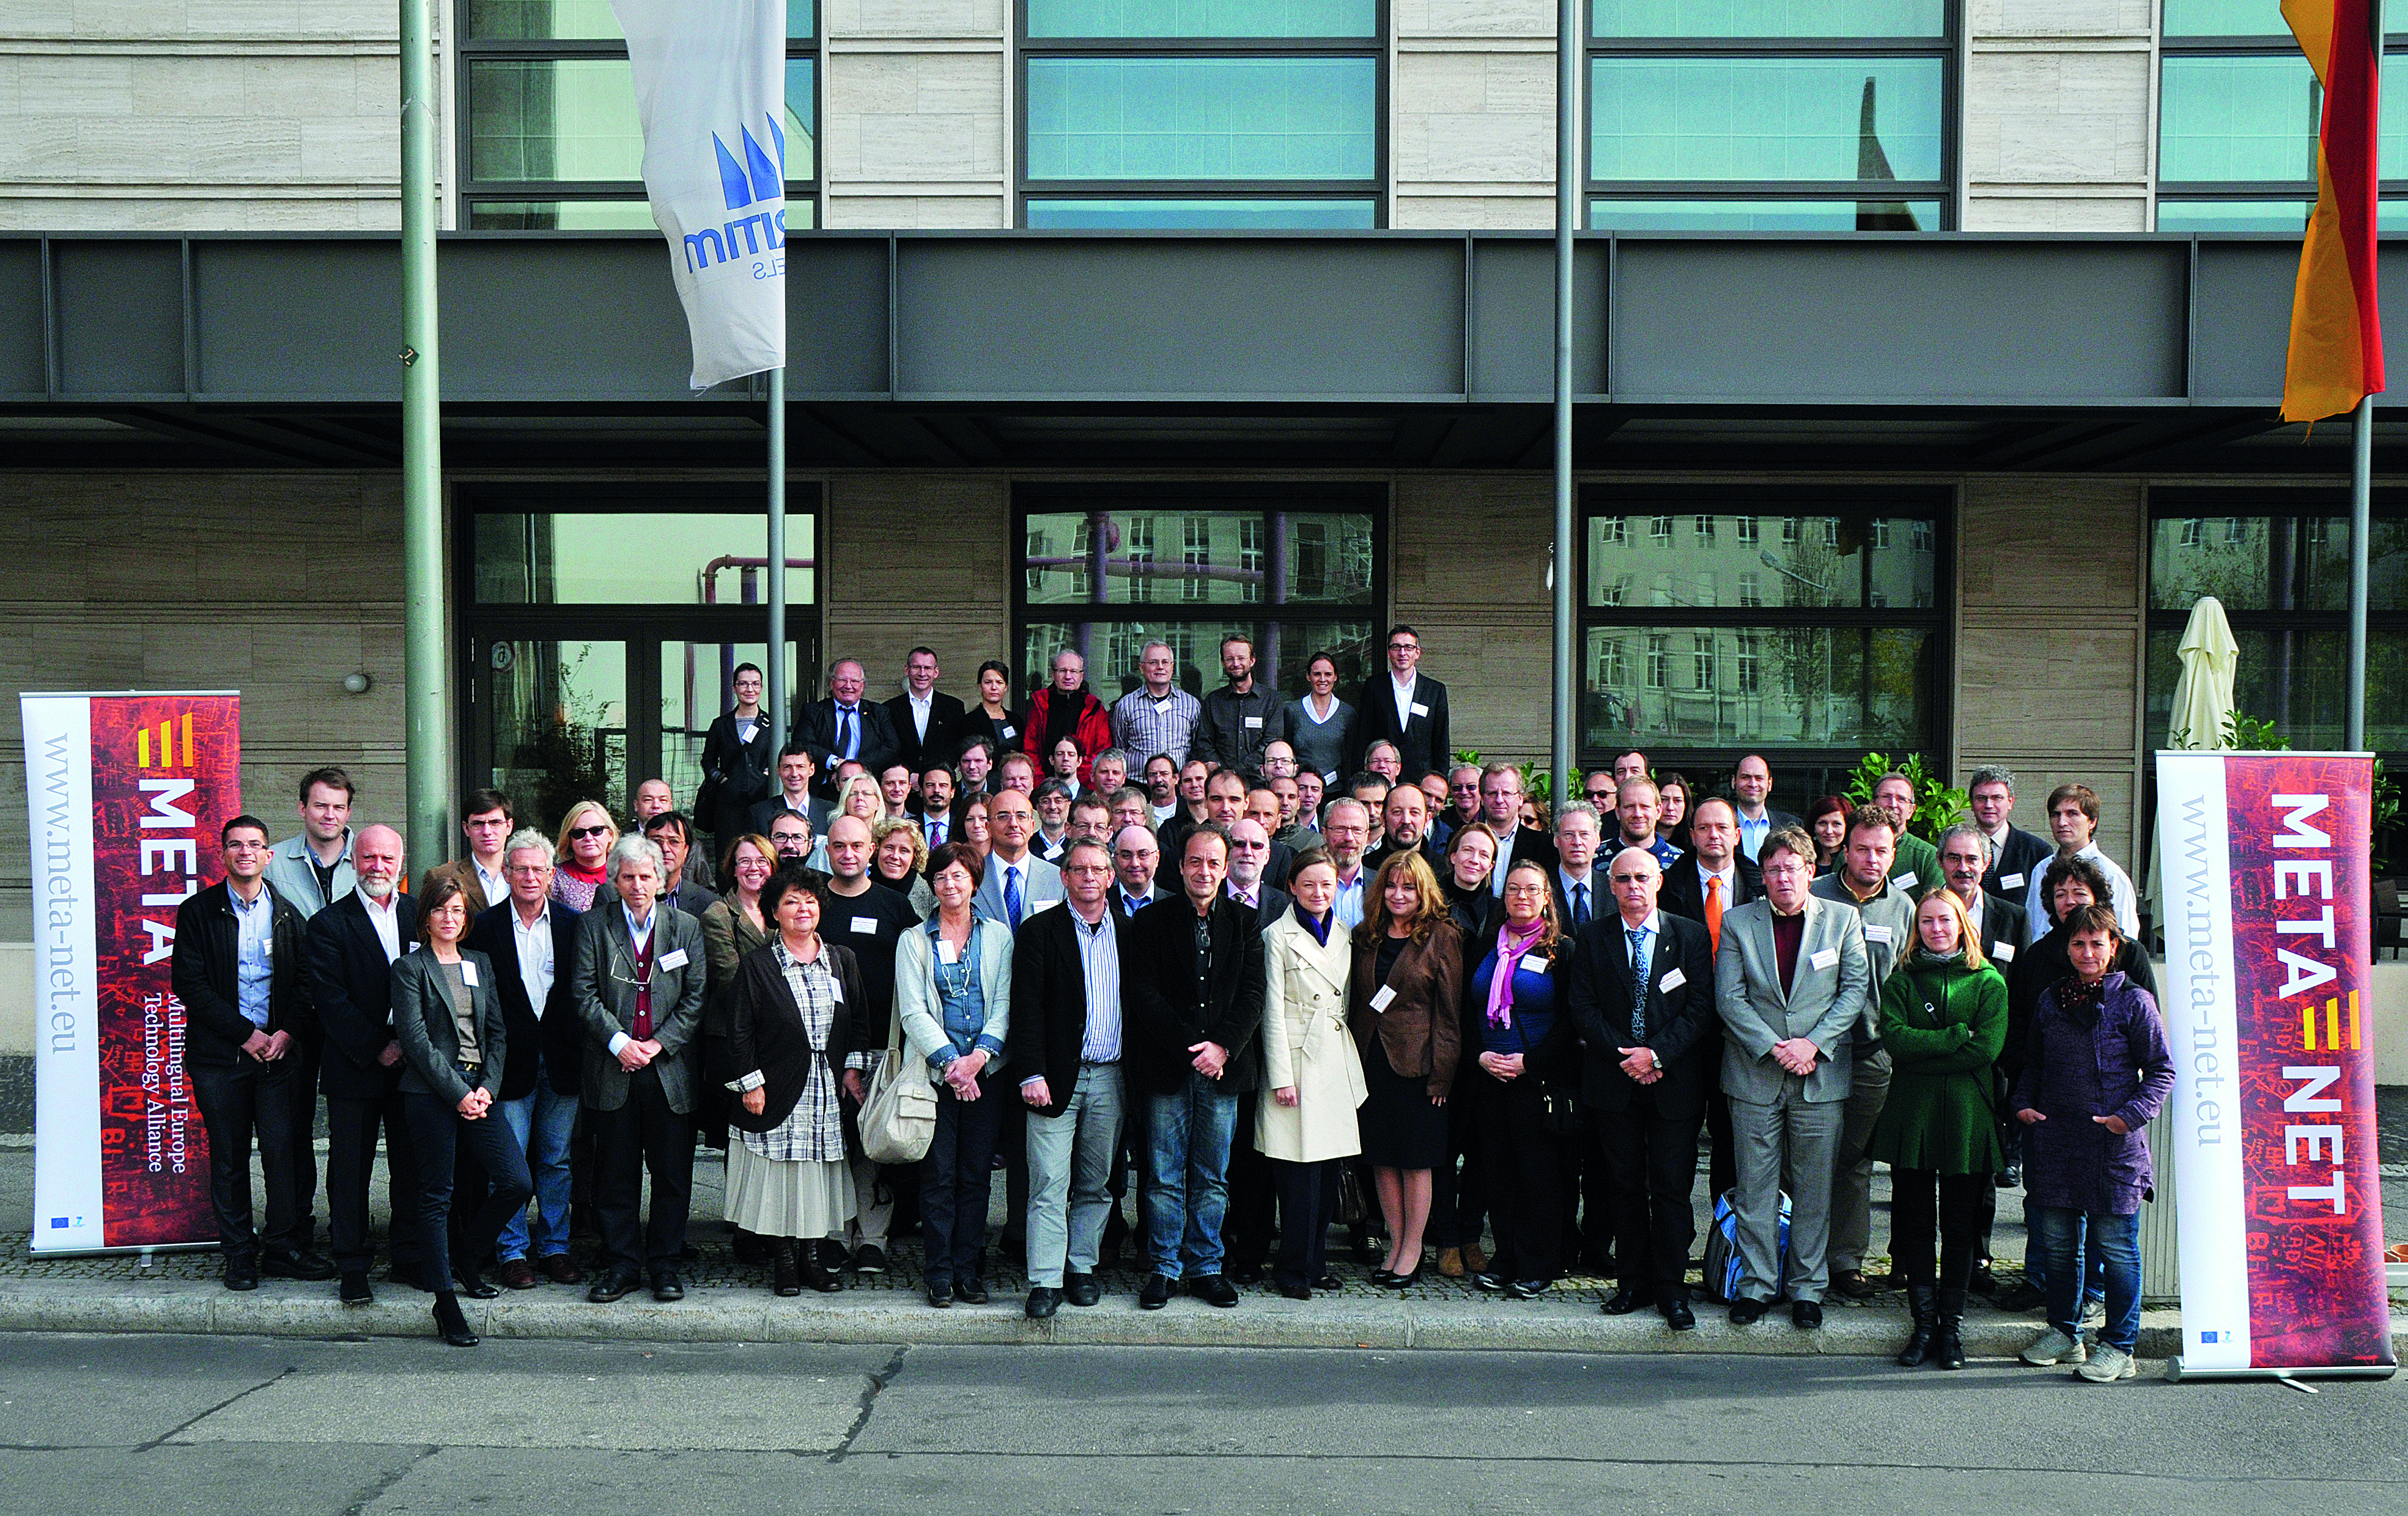
\includegraphics[width=\textwidth]{../_media/meta-net_team.jpg}
   \fbox{Dummy -- we'll include the group photo of our META-NET meeting in Berlin here}
  \caption{Cerca de 100 especialistas em Tecnologias da Linguagem -- representantes dos países e das línguas representados na META-NET -- discutiram e finalizaram os resultados-chave e a mensagem incluídos na Série Livro Branco no Encontro META-NET em Berlim, Alemanha, a 21/22 de Ou\-tu\-bro de 2011. --- \textcolor{grey1}{About 100 language technology experts -- representatives of the countries and languages represented in META-NET -- discussed and finalised the key results and messages of the White Paper Series at a META-NET meeting in Berlin, Germany, on October 21/22, 2011.}}
\end{figure*}

\cleardoublepage

\bsection[A Série Livro Branco META-NET -- The META-NET White Paper Series]{A Série Livro Branco META-NET --- The META-NET\ \ \ \ \ \ White Paper Series}
\label{whitepaperseries}

\vspace*{-5mm}
\centering
  \setlength{\tabcolsep}{2em}
  \begin{tabularx}{\textwidth}{lllll} \toprule\addlinespace
  %\begin{tabulary}{170mm}{LLL} \toprule
  &Alemão & German & Deutsch& \\
  &Basco & Basque & euskara& \\
  &Búlgaro & Bulgarian & български& \\
  &Catalão & Catalan & català& \\
  &Checo & Czech & čeština& \\
  &Croata & Croatian & hrvatski& \\
  &Dinamarquês & Danish & dansk& \\
  &Eslovaco & Slovak & slovenčina& \\
  &Esloveno & Slovene & slovenščina& \\
  &Espanhol & Spanish & español& \\
  &Estónio & Estonian & eesti& \\
  &Finlandês & Finnish & suomi& \\
  &Francês & French & français& \\
  &Galego & Galician & galego& \\
  &Grego & Greek & ελληνικά& \\
  &Húngaro & Hungarian & magyar& \\
  &Inglês & English & English& \\
  &Irlandês & Irish & Gaeilge& \\
  &Islandês & Icelandic & íslenska& \\
  &Italiano & Italian & italiano& \\
  &Letão & Latvian & latviešu valoda& \\
  &Lituano & Lithuanian & lietuvių kalba& \\
  &Maltês & Maltese & Malti& \\
  &Neerlandês & Dutch & Nederlands& \\
  &Norueguês Bokmål & Norwegian Bokmål & bokmål& \\
  &Norueguês Nynorsk & Norwegian Nynorsk & nynorsk& \\
  &Polaco & Polish & polski& \\
  &Português & Portuguese & português& \\
  &Romeno & Romanian & română& \\
  &Sérvio & Serbian & српски& \\
  &Sueco & Swedish & svenska& \\ \addlinespace \bottomrule
\end{tabularx}
